% Options for packages loaded elsewhere
\PassOptionsToPackage{unicode}{hyperref}
\PassOptionsToPackage{hyphens}{url}
%
\documentclass[
]{book}
\usepackage{amsmath,amssymb}
\usepackage{lmodern}
\usepackage{iftex}
\ifPDFTeX
  \usepackage[T1]{fontenc}
  \usepackage[utf8]{inputenc}
  \usepackage{textcomp} % provide euro and other symbols
\else % if luatex or xetex
  \usepackage{unicode-math}
  \defaultfontfeatures{Scale=MatchLowercase}
  \defaultfontfeatures[\rmfamily]{Ligatures=TeX,Scale=1}
\fi
% Use upquote if available, for straight quotes in verbatim environments
\IfFileExists{upquote.sty}{\usepackage{upquote}}{}
\IfFileExists{microtype.sty}{% use microtype if available
  \usepackage[]{microtype}
  \UseMicrotypeSet[protrusion]{basicmath} % disable protrusion for tt fonts
}{}
\makeatletter
\@ifundefined{KOMAClassName}{% if non-KOMA class
  \IfFileExists{parskip.sty}{%
    \usepackage{parskip}
  }{% else
    \setlength{\parindent}{0pt}
    \setlength{\parskip}{6pt plus 2pt minus 1pt}}
}{% if KOMA class
  \KOMAoptions{parskip=half}}
\makeatother
\usepackage{xcolor}
\IfFileExists{xurl.sty}{\usepackage{xurl}}{} % add URL line breaks if available
\IfFileExists{bookmark.sty}{\usepackage{bookmark}}{\usepackage{hyperref}}
\hypersetup{
  pdftitle={Advanced R Exercises},
  pdfauthor={Indrajeet Patil},
  hidelinks,
  pdfcreator={LaTeX via pandoc}}
\urlstyle{same} % disable monospaced font for URLs
\usepackage{color}
\usepackage{fancyvrb}
\newcommand{\VerbBar}{|}
\newcommand{\VERB}{\Verb[commandchars=\\\{\}]}
\DefineVerbatimEnvironment{Highlighting}{Verbatim}{commandchars=\\\{\}}
% Add ',fontsize=\small' for more characters per line
\usepackage{framed}
\definecolor{shadecolor}{RGB}{248,248,248}
\newenvironment{Shaded}{\begin{snugshade}}{\end{snugshade}}
\newcommand{\AlertTok}[1]{\textcolor[rgb]{0.94,0.16,0.16}{#1}}
\newcommand{\AnnotationTok}[1]{\textcolor[rgb]{0.56,0.35,0.01}{\textbf{\textit{#1}}}}
\newcommand{\AttributeTok}[1]{\textcolor[rgb]{0.77,0.63,0.00}{#1}}
\newcommand{\BaseNTok}[1]{\textcolor[rgb]{0.00,0.00,0.81}{#1}}
\newcommand{\BuiltInTok}[1]{#1}
\newcommand{\CharTok}[1]{\textcolor[rgb]{0.31,0.60,0.02}{#1}}
\newcommand{\CommentTok}[1]{\textcolor[rgb]{0.56,0.35,0.01}{\textit{#1}}}
\newcommand{\CommentVarTok}[1]{\textcolor[rgb]{0.56,0.35,0.01}{\textbf{\textit{#1}}}}
\newcommand{\ConstantTok}[1]{\textcolor[rgb]{0.00,0.00,0.00}{#1}}
\newcommand{\ControlFlowTok}[1]{\textcolor[rgb]{0.13,0.29,0.53}{\textbf{#1}}}
\newcommand{\DataTypeTok}[1]{\textcolor[rgb]{0.13,0.29,0.53}{#1}}
\newcommand{\DecValTok}[1]{\textcolor[rgb]{0.00,0.00,0.81}{#1}}
\newcommand{\DocumentationTok}[1]{\textcolor[rgb]{0.56,0.35,0.01}{\textbf{\textit{#1}}}}
\newcommand{\ErrorTok}[1]{\textcolor[rgb]{0.64,0.00,0.00}{\textbf{#1}}}
\newcommand{\ExtensionTok}[1]{#1}
\newcommand{\FloatTok}[1]{\textcolor[rgb]{0.00,0.00,0.81}{#1}}
\newcommand{\FunctionTok}[1]{\textcolor[rgb]{0.00,0.00,0.00}{#1}}
\newcommand{\ImportTok}[1]{#1}
\newcommand{\InformationTok}[1]{\textcolor[rgb]{0.56,0.35,0.01}{\textbf{\textit{#1}}}}
\newcommand{\KeywordTok}[1]{\textcolor[rgb]{0.13,0.29,0.53}{\textbf{#1}}}
\newcommand{\NormalTok}[1]{#1}
\newcommand{\OperatorTok}[1]{\textcolor[rgb]{0.81,0.36,0.00}{\textbf{#1}}}
\newcommand{\OtherTok}[1]{\textcolor[rgb]{0.56,0.35,0.01}{#1}}
\newcommand{\PreprocessorTok}[1]{\textcolor[rgb]{0.56,0.35,0.01}{\textit{#1}}}
\newcommand{\RegionMarkerTok}[1]{#1}
\newcommand{\SpecialCharTok}[1]{\textcolor[rgb]{0.00,0.00,0.00}{#1}}
\newcommand{\SpecialStringTok}[1]{\textcolor[rgb]{0.31,0.60,0.02}{#1}}
\newcommand{\StringTok}[1]{\textcolor[rgb]{0.31,0.60,0.02}{#1}}
\newcommand{\VariableTok}[1]{\textcolor[rgb]{0.00,0.00,0.00}{#1}}
\newcommand{\VerbatimStringTok}[1]{\textcolor[rgb]{0.31,0.60,0.02}{#1}}
\newcommand{\WarningTok}[1]{\textcolor[rgb]{0.56,0.35,0.01}{\textbf{\textit{#1}}}}
\usepackage{longtable,booktabs,array}
\usepackage{calc} % for calculating minipage widths
% Correct order of tables after \paragraph or \subparagraph
\usepackage{etoolbox}
\makeatletter
\patchcmd\longtable{\par}{\if@noskipsec\mbox{}\fi\par}{}{}
\makeatother
% Allow footnotes in longtable head/foot
\IfFileExists{footnotehyper.sty}{\usepackage{footnotehyper}}{\usepackage{footnote}}
\makesavenoteenv{longtable}
\usepackage{graphicx}
\makeatletter
\def\maxwidth{\ifdim\Gin@nat@width>\linewidth\linewidth\else\Gin@nat@width\fi}
\def\maxheight{\ifdim\Gin@nat@height>\textheight\textheight\else\Gin@nat@height\fi}
\makeatother
% Scale images if necessary, so that they will not overflow the page
% margins by default, and it is still possible to overwrite the defaults
% using explicit options in \includegraphics[width, height, ...]{}
\setkeys{Gin}{width=\maxwidth,height=\maxheight,keepaspectratio}
% Set default figure placement to htbp
\makeatletter
\def\fps@figure{htbp}
\makeatother
\setlength{\emergencystretch}{3em} % prevent overfull lines
\providecommand{\tightlist}{%
  \setlength{\itemsep}{0pt}\setlength{\parskip}{0pt}}
\setcounter{secnumdepth}{5}
\usepackage{booktabs}
\ifLuaTeX
  \usepackage{selnolig}  % disable illegal ligatures
\fi
\usepackage[]{natbib}
\bibliographystyle{apalike}

\title{Advanced R Exercises}
\author{Indrajeet Patil}
\date{2022-03-21}

\begin{document}
\maketitle

{
\setcounter{tocdepth}{1}
\tableofcontents
}
\hypertarget{about}{%
\chapter*{About}\label{about}}
\addcontentsline{toc}{chapter}{About}

My solutions to exercises from the \emph{Advanced R} (2nd Edition) \href{https://adv-r.hadley.nz/}{book}.

Note that you \textbf{should be} reading the \href{https://advanced-r-solutions.rbind.io/index.html}{official solutions manual}, which has more detailed explanations and are guaranteed to have correct solutions as the original author was also involved in writing them. I provide no such guarantees. 😬

\begin{itemize}
\item
  \href{https://github.com/IndrajeetPatil/Advanced-R-exercises}{My solutions}
\item
  \href{https://advanced-r-solutions.rbind.io/index.html}{Official solutions}
\end{itemize}

\hypertarget{introduction}{%
\chapter{Introduction}\label{introduction}}

No exercises.

\hypertarget{names-and-values}{%
\chapter{Names and values}\label{names-and-values}}

\hypertarget{exercises}{%
\section{2.2.2 Exercises}\label{exercises}}

\textbf{Q1.} Explain the relationship between \texttt{a}, \texttt{b}, \texttt{c} and \texttt{d} in the following code:

\begin{Shaded}
\begin{Highlighting}[]
\NormalTok{a }\OtherTok{\textless{}{-}} \DecValTok{1}\SpecialCharTok{:}\DecValTok{10}
\NormalTok{b }\OtherTok{\textless{}{-}}\NormalTok{ a}
\NormalTok{c }\OtherTok{\textless{}{-}}\NormalTok{ b}
\NormalTok{d }\OtherTok{\textless{}{-}} \DecValTok{1}\SpecialCharTok{:}\DecValTok{10}
\end{Highlighting}
\end{Shaded}

\textbf{A1.}

\begin{Shaded}
\begin{Highlighting}[]
\NormalTok{a }\OtherTok{\textless{}{-}} \DecValTok{1}\SpecialCharTok{:}\DecValTok{10}
\NormalTok{b }\OtherTok{\textless{}{-}}\NormalTok{ a}
\NormalTok{c }\OtherTok{\textless{}{-}}\NormalTok{ b}
\NormalTok{d }\OtherTok{\textless{}{-}} \DecValTok{1}\SpecialCharTok{:}\DecValTok{10}
\end{Highlighting}
\end{Shaded}

The names (\texttt{a}, \texttt{b}, and \texttt{c}) are references to the same object in memory, as can be seen by the identical memory address:

\begin{Shaded}
\begin{Highlighting}[]
\FunctionTok{library}\NormalTok{(lobstr)}

\FunctionTok{obj\_addrs}\NormalTok{(}\FunctionTok{list}\NormalTok{(a, b, c))}
\CommentTok{\#\textgreater{} [1] "0x11f138070" "0x11f138070" "0x11f138070"}
\end{Highlighting}
\end{Shaded}

Except \texttt{d}, which is a different object, even if it has the same value:

\begin{Shaded}
\begin{Highlighting}[]
\FunctionTok{obj\_addr}\NormalTok{(d)}
\CommentTok{\#\textgreater{} [1] "0x11f456310"}
\end{Highlighting}
\end{Shaded}

\textbf{Q2.} The following code accesses the mean function in multiple ways. Do they all point to the same underlying function object? Verify this with \texttt{lobstr::obj\_addr()}.

\begin{Shaded}
\begin{Highlighting}[]
\NormalTok{mean}
\NormalTok{base}\SpecialCharTok{::}\NormalTok{mean}
\FunctionTok{get}\NormalTok{(}\StringTok{"mean"}\NormalTok{)}
\FunctionTok{evalq}\NormalTok{(mean)}
\FunctionTok{match.fun}\NormalTok{(}\StringTok{"mean"}\NormalTok{)}
\end{Highlighting}
\end{Shaded}

\textbf{A2.}

Following code verifies that indeed these calls all point to the same underlying function object.

\begin{Shaded}
\begin{Highlighting}[]
\FunctionTok{obj\_addr}\NormalTok{(mean)}
\CommentTok{\#\textgreater{} [1] "0x10eb66338"}
\FunctionTok{obj\_addr}\NormalTok{(base}\SpecialCharTok{::}\NormalTok{mean)}
\CommentTok{\#\textgreater{} [1] "0x10eb66338"}
\FunctionTok{obj\_addr}\NormalTok{(}\FunctionTok{get}\NormalTok{(}\StringTok{"mean"}\NormalTok{))}
\CommentTok{\#\textgreater{} [1] "0x10eb66338"}
\FunctionTok{obj\_addr}\NormalTok{(}\FunctionTok{evalq}\NormalTok{(mean))}
\CommentTok{\#\textgreater{} [1] "0x10eb66338"}
\FunctionTok{obj\_addr}\NormalTok{(}\FunctionTok{match.fun}\NormalTok{(}\StringTok{"mean"}\NormalTok{))}
\CommentTok{\#\textgreater{} [1] "0x10eb66338"}
\end{Highlighting}
\end{Shaded}

\textbf{Q3.} By default, base R data import functions, like \texttt{read.csv()}, will automatically convert non-syntactic names to syntactic ones. Why might this be problematic? What option allows you to suppress this behaviour?

\textbf{A3.}

The conversion of non-syntactic names to syntactic ones can sometimes corrupt the data. Some datasets may require non-syntactic names.

To suppress this behavior, one can set \texttt{check.names\ =\ FALSE}.

\textbf{Q4.} What rules does \texttt{make.names()} use to convert non-syntactic names into syntactic ones?

\textbf{A4.}

It just prepends \texttt{X} in non-syntactic names and invalid characters (like \texttt{@}) are converted to \texttt{.}.

\begin{Shaded}
\begin{Highlighting}[]
\FunctionTok{make.names}\NormalTok{(}\FunctionTok{c}\NormalTok{(}\StringTok{"123abc"}\NormalTok{, }\StringTok{"@me"}\NormalTok{, }\StringTok{"\_yu"}\NormalTok{, }\StringTok{"  gh"}\NormalTok{, }\StringTok{"else"}\NormalTok{))}
\CommentTok{\#\textgreater{} [1] "X123abc" "X.me"    "X\_yu"    "X..gh"   "else."}
\end{Highlighting}
\end{Shaded}

\textbf{Q5.} I slightly simplified the rules that govern syntactic names. Why is \texttt{.123e1} not a syntactic name? Read \texttt{?make.names} for the full details.

\textbf{A5.}

Because it is parsed as a number.

\begin{Shaded}
\begin{Highlighting}[]
\FunctionTok{typeof}\NormalTok{(.}\FloatTok{123e1}\NormalTok{)}
\CommentTok{\#\textgreater{} [1] "double"}
\end{Highlighting}
\end{Shaded}

And as the docs mention (emphasis mine):

\begin{quote}
A syntactically valid name consists of letters, numbers and the dot or underline characters and starts with a letter or \textbf{the dot not followed by a number}.
\end{quote}

Here is how \texttt{make.names()} will make it syntactic:

\begin{Shaded}
\begin{Highlighting}[]
\FunctionTok{make.names}\NormalTok{(.}\FloatTok{123e1}\NormalTok{)}
\CommentTok{\#\textgreater{} [1] "X1.23"}
\end{Highlighting}
\end{Shaded}

\hypertarget{exercises-1}{%
\section{2.3.6 Exercises}\label{exercises-1}}

\textbf{Q1.} Why is \texttt{tracemem(1:10)} not useful?

\textbf{A1.}

\texttt{tracemem()} traces copying of objects in R, but since the object created here is not assigned a name, there is nothing to trace.

\begin{Shaded}
\begin{Highlighting}[]
\FunctionTok{tracemem}\NormalTok{(}\DecValTok{1}\SpecialCharTok{:}\DecValTok{10}\NormalTok{)}
\CommentTok{\#\textgreater{} [1] "\textless{}0x10f281738\textgreater{}"}
\end{Highlighting}
\end{Shaded}

\textbf{Q2.} Explain why \texttt{tracemem()} shows two copies when you run this code. Hint: carefully look at the difference between this code and the code shown earlier in the section.

\begin{Shaded}
\begin{Highlighting}[]
\NormalTok{x }\OtherTok{\textless{}{-}} \FunctionTok{c}\NormalTok{(1L, 2L, 3L)}
\FunctionTok{tracemem}\NormalTok{(x)}

\NormalTok{x[[}\DecValTok{3}\NormalTok{]] }\OtherTok{\textless{}{-}} \DecValTok{4}
\end{Highlighting}
\end{Shaded}

\textbf{A2.}

Were it not for \texttt{4} being a double - and not an integer (\texttt{4L}) - this would have been modified in place.

\begin{Shaded}
\begin{Highlighting}[]
\NormalTok{x }\OtherTok{\textless{}{-}} \FunctionTok{c}\NormalTok{(1L, 2L, 3L)}
\FunctionTok{tracemem}\NormalTok{(x)}
\CommentTok{\#\textgreater{} [1] "\textless{}0x11a2e0fc8\textgreater{}"}

\NormalTok{x[[}\DecValTok{3}\NormalTok{]] }\OtherTok{\textless{}{-}} \DecValTok{4}
\CommentTok{\#\textgreater{} tracemem[0x11a2e0fc8 {-}\textgreater{} 0x10f6678c8]: eval eval eval\_with\_user\_handlers withVisible withCallingHandlers handle timing\_fn evaluate\_call \textless{}Anonymous\textgreater{} evaluate in\_dir eng\_r block\_exec call\_block process\_group.block process\_group withCallingHandlers process\_file \textless{}Anonymous\textgreater{} \textless{}Anonymous\textgreater{} do.call eval eval eval eval eval.parent local }
\CommentTok{\#\textgreater{} tracemem[0x10f6678c8 {-}\textgreater{} 0x119daf008]: eval eval eval\_with\_user\_handlers withVisible withCallingHandlers handle timing\_fn evaluate\_call \textless{}Anonymous\textgreater{} evaluate in\_dir eng\_r block\_exec call\_block process\_group.block process\_group withCallingHandlers process\_file \textless{}Anonymous\textgreater{} \textless{}Anonymous\textgreater{} do.call eval eval eval eval eval.parent local}
\end{Highlighting}
\end{Shaded}

Try with integer:

\begin{Shaded}
\begin{Highlighting}[]
\NormalTok{x }\OtherTok{\textless{}{-}} \FunctionTok{c}\NormalTok{(1L, 2L, 3L)}
\FunctionTok{tracemem}\NormalTok{(x)}
\CommentTok{\#\textgreater{} [1] "\textless{}0x119d8e908\textgreater{}"}

\NormalTok{x[[}\DecValTok{3}\NormalTok{]] }\OtherTok{\textless{}{-}}\NormalTok{ 4L}
\CommentTok{\#\textgreater{} tracemem[0x119d8e908 {-}\textgreater{} 0x119b244c8]: eval eval eval\_with\_user\_handlers withVisible withCallingHandlers handle timing\_fn evaluate\_call \textless{}Anonymous\textgreater{} evaluate in\_dir eng\_r block\_exec call\_block process\_group.block process\_group withCallingHandlers process\_file \textless{}Anonymous\textgreater{} \textless{}Anonymous\textgreater{} do.call eval eval eval eval eval.parent local}
\end{Highlighting}
\end{Shaded}

As for why this still produces a copy, this is from Solutions manual:

\begin{quote}
Please be aware that running this code in RStudio will result in additional copies because of the reference from the environment pane.
\end{quote}

\textbf{Q3.} Sketch out the relationship between the following objects:

\begin{Shaded}
\begin{Highlighting}[]
\NormalTok{a }\OtherTok{\textless{}{-}} \DecValTok{1}\SpecialCharTok{:}\DecValTok{10}
\NormalTok{b }\OtherTok{\textless{}{-}} \FunctionTok{list}\NormalTok{(a, a)}
\NormalTok{c }\OtherTok{\textless{}{-}} \FunctionTok{list}\NormalTok{(b, a, }\DecValTok{1}\SpecialCharTok{:}\DecValTok{10}\NormalTok{)}
\end{Highlighting}
\end{Shaded}

\textbf{A3.}

\begin{Shaded}
\begin{Highlighting}[]
\NormalTok{a }\OtherTok{\textless{}{-}} \DecValTok{1}\SpecialCharTok{:}\DecValTok{10}
\NormalTok{b }\OtherTok{\textless{}{-}} \FunctionTok{list}\NormalTok{(a, a)}
\NormalTok{c }\OtherTok{\textless{}{-}} \FunctionTok{list}\NormalTok{(b, a, }\DecValTok{1}\SpecialCharTok{:}\DecValTok{10}\NormalTok{)}

\FunctionTok{ref}\NormalTok{(a)}
\CommentTok{\#\textgreater{} [1:0x118a941e8] \textless{}int\textgreater{}}

\FunctionTok{ref}\NormalTok{(b)}
\CommentTok{\#\textgreater{} █ [1:0x119f78488] \textless{}list\textgreater{} }
\CommentTok{\#\textgreater{} ├─[2:0x118a941e8] \textless{}int\textgreater{} }
\CommentTok{\#\textgreater{} └─[2:0x118a941e8]}

\FunctionTok{ref}\NormalTok{(c)}
\CommentTok{\#\textgreater{} █ [1:0x118ec5958] \textless{}list\textgreater{} }
\CommentTok{\#\textgreater{} ├─█ [2:0x119f78488] \textless{}list\textgreater{} }
\CommentTok{\#\textgreater{} │ ├─[3:0x118a941e8] \textless{}int\textgreater{} }
\CommentTok{\#\textgreater{} │ └─[3:0x118a941e8] }
\CommentTok{\#\textgreater{} ├─[3:0x118a941e8] }
\CommentTok{\#\textgreater{} └─[4:0x118c1f1d0] \textless{}int\textgreater{}}
\end{Highlighting}
\end{Shaded}

\textbf{Q4.} What happens when you run this code?

\begin{Shaded}
\begin{Highlighting}[]
\NormalTok{x }\OtherTok{\textless{}{-}} \FunctionTok{list}\NormalTok{(}\DecValTok{1}\SpecialCharTok{:}\DecValTok{10}\NormalTok{)}
\NormalTok{x[[}\DecValTok{2}\NormalTok{]] }\OtherTok{\textless{}{-}}\NormalTok{ x}
\end{Highlighting}
\end{Shaded}

Draw a picture.

\textbf{A4.}

\begin{Shaded}
\begin{Highlighting}[]
\NormalTok{x }\OtherTok{\textless{}{-}} \FunctionTok{list}\NormalTok{(}\DecValTok{1}\SpecialCharTok{:}\DecValTok{10}\NormalTok{)}
\NormalTok{x}
\CommentTok{\#\textgreater{} [[1]]}
\CommentTok{\#\textgreater{}  [1]  1  2  3  4  5  6  7  8  9 10}
\FunctionTok{obj\_addr}\NormalTok{(x)}
\CommentTok{\#\textgreater{} [1] "0x10ff41388"}

\NormalTok{x[[}\DecValTok{2}\NormalTok{]] }\OtherTok{\textless{}{-}}\NormalTok{ x}
\NormalTok{x}
\CommentTok{\#\textgreater{} [[1]]}
\CommentTok{\#\textgreater{}  [1]  1  2  3  4  5  6  7  8  9 10}
\CommentTok{\#\textgreater{} }
\CommentTok{\#\textgreater{} [[2]]}
\CommentTok{\#\textgreater{} [[2]][[1]]}
\CommentTok{\#\textgreater{}  [1]  1  2  3  4  5  6  7  8  9 10}
\FunctionTok{obj\_addr}\NormalTok{(x)}
\CommentTok{\#\textgreater{} [1] "0x11a2a6ac8"}

\FunctionTok{ref}\NormalTok{(x)}
\CommentTok{\#\textgreater{} █ [1:0x11a2a6ac8] \textless{}list\textgreater{} }
\CommentTok{\#\textgreater{} ├─[2:0x11f79c1c0] \textless{}int\textgreater{} }
\CommentTok{\#\textgreater{} └─█ [3:0x10ff41388] \textless{}list\textgreater{} }
\CommentTok{\#\textgreater{}   └─[2:0x11f79c1c0]}
\end{Highlighting}
\end{Shaded}

Figure from the official solution manual can be found here:
\url{https://advanced-r-solutions.rbind.io/images/names_values/copy_on_modify_fig2.png}

\hypertarget{exercises-2}{%
\section{2.4.1 Exercises}\label{exercises-2}}

\textbf{Q1.} In the following example, why are \texttt{object.size(y)} and \texttt{obj\_size(y)} so radically different? Consult the documentation of \texttt{object.size()}.

\begin{Shaded}
\begin{Highlighting}[]
\NormalTok{y }\OtherTok{\textless{}{-}} \FunctionTok{rep}\NormalTok{(}\FunctionTok{list}\NormalTok{(}\FunctionTok{runif}\NormalTok{(}\FloatTok{1e4}\NormalTok{)), }\DecValTok{100}\NormalTok{)}

\FunctionTok{object.size}\NormalTok{(y)}
\FunctionTok{obj\_size}\NormalTok{(y)}
\end{Highlighting}
\end{Shaded}

\textbf{A1.}

\begin{quote}
This function\ldots does not detect if elements of a list are shared.
\end{quote}

\begin{Shaded}
\begin{Highlighting}[]
\NormalTok{y }\OtherTok{\textless{}{-}} \FunctionTok{rep}\NormalTok{(}\FunctionTok{list}\NormalTok{(}\FunctionTok{runif}\NormalTok{(}\FloatTok{1e4}\NormalTok{)), }\DecValTok{100}\NormalTok{)}

\FunctionTok{object.size}\NormalTok{(y)}
\CommentTok{\#\textgreater{} 8005648 bytes}

\FunctionTok{obj\_size}\NormalTok{(y)}
\CommentTok{\#\textgreater{} 80,896 B}
\end{Highlighting}
\end{Shaded}

\textbf{Q2.} Take the following list. Why is its size somewhat misleading?

\begin{Shaded}
\begin{Highlighting}[]
\NormalTok{funs }\OtherTok{\textless{}{-}} \FunctionTok{list}\NormalTok{(mean, sd, var)}
\FunctionTok{obj\_size}\NormalTok{(funs)}
\end{Highlighting}
\end{Shaded}

\textbf{A2.}

These functions are not externally created objects in R, but are always available, so doesn't make much sense to measure their size.

\begin{Shaded}
\begin{Highlighting}[]
\NormalTok{funs }\OtherTok{\textless{}{-}} \FunctionTok{list}\NormalTok{(mean, sd, var)}
\FunctionTok{obj\_size}\NormalTok{(funs)}
\CommentTok{\#\textgreater{} 17,608 B}
\end{Highlighting}
\end{Shaded}

Nevertheless, it's still interesting that the addition is not the same as size of list of those objects.

\begin{Shaded}
\begin{Highlighting}[]
\FunctionTok{obj\_size}\NormalTok{(mean)}
\CommentTok{\#\textgreater{} 1,184 B}
\FunctionTok{obj\_size}\NormalTok{(sd)}
\CommentTok{\#\textgreater{} 4,480 B}
\FunctionTok{obj\_size}\NormalTok{(var)}
\CommentTok{\#\textgreater{} 12,472 B}

\FunctionTok{obj\_size}\NormalTok{(mean) }\SpecialCharTok{+} \FunctionTok{obj\_size}\NormalTok{(sd) }\SpecialCharTok{+} \FunctionTok{obj\_size}\NormalTok{(var)}
\CommentTok{\#\textgreater{} 18,136 B}
\end{Highlighting}
\end{Shaded}

\textbf{Q3.} Predict the output of the following code:

\begin{Shaded}
\begin{Highlighting}[]
\NormalTok{a }\OtherTok{\textless{}{-}} \FunctionTok{runif}\NormalTok{(}\FloatTok{1e6}\NormalTok{)}
\FunctionTok{obj\_size}\NormalTok{(a)}

\NormalTok{b }\OtherTok{\textless{}{-}} \FunctionTok{list}\NormalTok{(a, a)}
\FunctionTok{obj\_size}\NormalTok{(b)}
\FunctionTok{obj\_size}\NormalTok{(a, b)}

\NormalTok{b[[}\DecValTok{1}\NormalTok{]][[}\DecValTok{1}\NormalTok{]] }\OtherTok{\textless{}{-}} \DecValTok{10}
\FunctionTok{obj\_size}\NormalTok{(b)}
\FunctionTok{obj\_size}\NormalTok{(a, b)}

\NormalTok{b[[}\DecValTok{2}\NormalTok{]][[}\DecValTok{1}\NormalTok{]] }\OtherTok{\textless{}{-}} \DecValTok{10}
\FunctionTok{obj\_size}\NormalTok{(b)}
\FunctionTok{obj\_size}\NormalTok{(a, b)}
\end{Highlighting}
\end{Shaded}

\textbf{A3.} Correctly predicted 😉

\begin{Shaded}
\begin{Highlighting}[]
\NormalTok{a }\OtherTok{\textless{}{-}} \FunctionTok{runif}\NormalTok{(}\FloatTok{1e6}\NormalTok{)}
\FunctionTok{obj\_size}\NormalTok{(a)}
\CommentTok{\#\textgreater{} 8,000,048 B}

\NormalTok{b }\OtherTok{\textless{}{-}} \FunctionTok{list}\NormalTok{(a, a)}
\FunctionTok{obj\_size}\NormalTok{(b)}
\CommentTok{\#\textgreater{} 8,000,112 B}
\FunctionTok{obj\_size}\NormalTok{(a, b)}
\CommentTok{\#\textgreater{} 8,000,112 B}

\NormalTok{b[[}\DecValTok{1}\NormalTok{]][[}\DecValTok{1}\NormalTok{]] }\OtherTok{\textless{}{-}} \DecValTok{10}
\FunctionTok{obj\_size}\NormalTok{(b)}
\CommentTok{\#\textgreater{} 16,000,160 B}
\FunctionTok{obj\_size}\NormalTok{(a, b)}
\CommentTok{\#\textgreater{} 16,000,160 B}

\NormalTok{b[[}\DecValTok{2}\NormalTok{]][[}\DecValTok{1}\NormalTok{]] }\OtherTok{\textless{}{-}} \DecValTok{10}
\FunctionTok{obj\_size}\NormalTok{(b)}
\CommentTok{\#\textgreater{} 16,000,160 B}
\FunctionTok{obj\_size}\NormalTok{(a, b)}
\CommentTok{\#\textgreater{} 24,000,208 B}
\end{Highlighting}
\end{Shaded}

\hypertarget{exercises-3}{%
\section{2.5.3 Exercises}\label{exercises-3}}

\textbf{Q1.} Explain why the following code doesn't create a circular list.

\begin{Shaded}
\begin{Highlighting}[]
\NormalTok{x }\OtherTok{\textless{}{-}} \FunctionTok{list}\NormalTok{()}
\NormalTok{x[[}\DecValTok{1}\NormalTok{]] }\OtherTok{\textless{}{-}}\NormalTok{ x}
\end{Highlighting}
\end{Shaded}

\textbf{A1.}

Copy-on-modify prevents the creation of a circular list.

\begin{Shaded}
\begin{Highlighting}[]
\NormalTok{x }\OtherTok{\textless{}{-}} \FunctionTok{list}\NormalTok{()}

\FunctionTok{obj\_addr}\NormalTok{(x)}
\CommentTok{\#\textgreater{} [1] "0x1189fcd88"}

\FunctionTok{tracemem}\NormalTok{(x)}
\CommentTok{\#\textgreater{} [1] "\textless{}0x1189fcd88\textgreater{}"}

\NormalTok{x[[}\DecValTok{1}\NormalTok{]] }\OtherTok{\textless{}{-}}\NormalTok{ x}
\CommentTok{\#\textgreater{} tracemem[0x1189fcd88 {-}\textgreater{} 0x118bac2b8]: eval eval eval\_with\_user\_handlers withVisible withCallingHandlers handle timing\_fn evaluate\_call \textless{}Anonymous\textgreater{} evaluate in\_dir eng\_r block\_exec call\_block process\_group.block process\_group withCallingHandlers process\_file \textless{}Anonymous\textgreater{} \textless{}Anonymous\textgreater{} do.call eval eval eval eval eval.parent local}

\FunctionTok{obj\_addr}\NormalTok{(x[[}\DecValTok{1}\NormalTok{]])}
\CommentTok{\#\textgreater{} [1] "0x1189fcd88"}
\end{Highlighting}
\end{Shaded}

\textbf{Q2.} Wrap the two methods for subtracting medians into two functions, then use the `bench' package to carefully compare their speeds. How does performance change as the number of columns increase?

\textbf{A2.}

Let's first microbenchmark functions that do and do not create copies for varying lengths of number of columns.

\begin{Shaded}
\begin{Highlighting}[]
\FunctionTok{library}\NormalTok{(bench)}
\FunctionTok{library}\NormalTok{(tidyverse)}

\NormalTok{generateDataFrame }\OtherTok{\textless{}{-}} \ControlFlowTok{function}\NormalTok{(ncol) \{}
  \FunctionTok{as.data.frame}\NormalTok{(}\FunctionTok{matrix}\NormalTok{(}\FunctionTok{runif}\NormalTok{(}\DecValTok{100} \SpecialCharTok{*}\NormalTok{ ncol), }\AttributeTok{nrow =} \DecValTok{100}\NormalTok{))}
\NormalTok{\}}

\NormalTok{withCopy }\OtherTok{\textless{}{-}} \ControlFlowTok{function}\NormalTok{(ncol) \{}
\NormalTok{  x }\OtherTok{\textless{}{-}} \FunctionTok{generateDataFrame}\NormalTok{(ncol)}
\NormalTok{  medians }\OtherTok{\textless{}{-}} \FunctionTok{vapply}\NormalTok{(x, median, }\FunctionTok{numeric}\NormalTok{(}\DecValTok{1}\NormalTok{))}

  \ControlFlowTok{for}\NormalTok{ (i }\ControlFlowTok{in} \FunctionTok{seq\_along}\NormalTok{(medians)) \{}
\NormalTok{    x[[i]] }\OtherTok{\textless{}{-}}\NormalTok{ x[[i]] }\SpecialCharTok{{-}}\NormalTok{ medians[[i]]}
\NormalTok{  \}}

  \FunctionTok{return}\NormalTok{(x)}
\NormalTok{\}}

\NormalTok{withoutCopy }\OtherTok{\textless{}{-}} \ControlFlowTok{function}\NormalTok{(ncol) \{}
\NormalTok{  x }\OtherTok{\textless{}{-}} \FunctionTok{generateDataFrame}\NormalTok{(ncol)}
\NormalTok{  medians }\OtherTok{\textless{}{-}} \FunctionTok{vapply}\NormalTok{(x, median, }\FunctionTok{numeric}\NormalTok{(}\DecValTok{1}\NormalTok{))}

\NormalTok{  y }\OtherTok{\textless{}{-}} \FunctionTok{as.list}\NormalTok{(x)}

  \ControlFlowTok{for}\NormalTok{ (i }\ControlFlowTok{in} \FunctionTok{seq\_along}\NormalTok{(medians)) \{}
\NormalTok{    y[[i]] }\OtherTok{\textless{}{-}}\NormalTok{ y[[i]] }\SpecialCharTok{{-}}\NormalTok{ medians[[i]]}
\NormalTok{  \}}

  \FunctionTok{return}\NormalTok{(y)}
\NormalTok{\}}

\NormalTok{benchComparison }\OtherTok{\textless{}{-}} \ControlFlowTok{function}\NormalTok{(ncol) \{}
\NormalTok{  bench}\SpecialCharTok{::}\FunctionTok{mark}\NormalTok{(}
    \FunctionTok{withCopy}\NormalTok{(ncol),}
    \FunctionTok{withoutCopy}\NormalTok{(ncol),}
    \AttributeTok{iterations =} \DecValTok{100}\NormalTok{,}
    \AttributeTok{check =} \ConstantTok{FALSE}
\NormalTok{  ) }\SpecialCharTok{\%\textgreater{}\%}
\NormalTok{    dplyr}\SpecialCharTok{::}\FunctionTok{select}\NormalTok{(expression}\SpecialCharTok{:}\NormalTok{total\_time)}
\NormalTok{\}}

\NormalTok{nColList }\OtherTok{\textless{}{-}} \FunctionTok{list}\NormalTok{(}\DecValTok{1}\NormalTok{, }\DecValTok{10}\NormalTok{, }\DecValTok{50}\NormalTok{, }\DecValTok{100}\NormalTok{, }\DecValTok{250}\NormalTok{, }\DecValTok{500}\NormalTok{, }\DecValTok{1000}\NormalTok{)}

\FunctionTok{names}\NormalTok{(nColList) }\OtherTok{\textless{}{-}} \FunctionTok{as.character}\NormalTok{(nColList)}

\NormalTok{benchDf }\OtherTok{\textless{}{-}}\NormalTok{ purrr}\SpecialCharTok{::}\FunctionTok{map\_dfr}\NormalTok{(}
  \AttributeTok{.x =}\NormalTok{ nColList,}
  \AttributeTok{.f =}\NormalTok{ benchComparison,}
  \AttributeTok{.id =} \StringTok{"nColumns"}
\NormalTok{)}
\end{Highlighting}
\end{Shaded}

Plotting these benchmarks reveals how the performance gets increasingly worse as the number of dataframes increases:

\begin{Shaded}
\begin{Highlighting}[]
\FunctionTok{ggplot}\NormalTok{(}
\NormalTok{  benchDf,}
  \FunctionTok{aes}\NormalTok{(}
    \AttributeTok{x =} \FunctionTok{as.numeric}\NormalTok{(nColumns),}
    \AttributeTok{y =}\NormalTok{ median,}
    \AttributeTok{group =} \FunctionTok{as.character}\NormalTok{(expression),}
    \AttributeTok{color =} \FunctionTok{as.character}\NormalTok{(expression)}
\NormalTok{  )}
\NormalTok{) }\SpecialCharTok{+}
  \FunctionTok{geom\_line}\NormalTok{() }\SpecialCharTok{+}
  \FunctionTok{labs}\NormalTok{(}
    \AttributeTok{x =} \StringTok{"Number of Columns"}\NormalTok{,}
    \AttributeTok{y =} \StringTok{"Median Execution Time (ms)"}\NormalTok{,}
    \AttributeTok{colour =} \StringTok{"Type of function"}
\NormalTok{  )}
\end{Highlighting}
\end{Shaded}

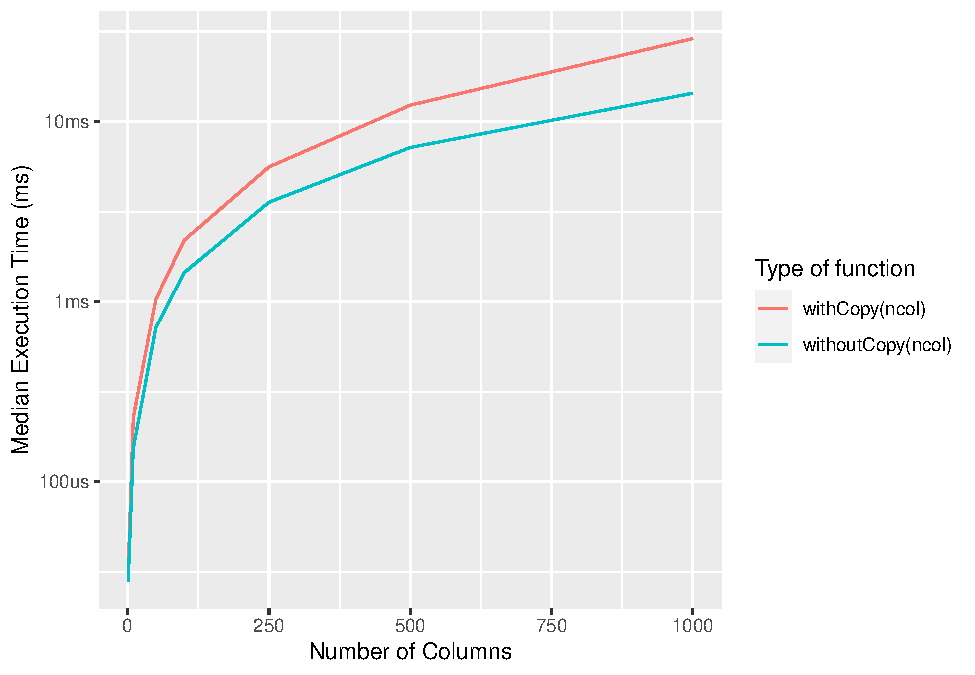
\includegraphics{Names-values_files/figure-latex/unnamed-chunk-29-1.pdf}

\textbf{Q3.} What happens if you attempt to use \texttt{tracemem()} on an environment?

\textbf{A3.}

It doesn't work and the documentation makes it clear as to why:

\begin{quote}
It is not useful to trace NULL, environments, promises, weak references, or external pointer objects, as these are not duplicated
\end{quote}

\begin{Shaded}
\begin{Highlighting}[]
\NormalTok{e }\OtherTok{\textless{}{-}}\NormalTok{ rlang}\SpecialCharTok{::}\FunctionTok{env}\NormalTok{(}\AttributeTok{a =} \DecValTok{1}\NormalTok{, }\AttributeTok{b =} \StringTok{"3"}\NormalTok{)}
\FunctionTok{tracemem}\NormalTok{(e)}
\CommentTok{\#\textgreater{} Error in tracemem(e): \textquotesingle{}tracemem\textquotesingle{} is not useful for promise and environment objects}
\end{Highlighting}
\end{Shaded}

\hypertarget{vectors}{%
\chapter{Vectors}\label{vectors}}

\hypertarget{exercise-3.2.5}{%
\section{Exercise 3.2.5}\label{exercise-3.2.5}}

\textbf{Q1.} Create raw and complex scalars

The raw type holds raw bytes. For example,

\begin{Shaded}
\begin{Highlighting}[]
\NormalTok{x }\OtherTok{\textless{}{-}} \StringTok{"A string"}

\NormalTok{(y }\OtherTok{\textless{}{-}} \FunctionTok{charToRaw}\NormalTok{(x))}
\CommentTok{\#\textgreater{} [1] 41 20 73 74 72 69 6e 67}

\FunctionTok{typeof}\NormalTok{(y)}
\CommentTok{\#\textgreater{} [1] "raw"}
\end{Highlighting}
\end{Shaded}

You can use it to also figure out differences in similar characters:

\begin{Shaded}
\begin{Highlighting}[]
\FunctionTok{charToRaw}\NormalTok{(}\StringTok{"–"}\NormalTok{) }\CommentTok{\# en{-}dash}
\CommentTok{\#\textgreater{} [1] e2 80 93}
\FunctionTok{charToRaw}\NormalTok{(}\StringTok{"—"}\NormalTok{) }\CommentTok{\# em{-}dash}
\CommentTok{\#\textgreater{} [1] e2 80 94}
\end{Highlighting}
\end{Shaded}

Complex vectors can be used to represent (surprise!) complex numbers.

Example of a complex scalar:

\begin{Shaded}
\begin{Highlighting}[]
\NormalTok{(x }\OtherTok{\textless{}{-}} \FunctionTok{complex}\NormalTok{(}\AttributeTok{length.out =} \DecValTok{1}\NormalTok{, }\AttributeTok{real =} \DecValTok{1}\NormalTok{, }\AttributeTok{imaginary =} \DecValTok{8}\NormalTok{))}
\CommentTok{\#\textgreater{} [1] 1+8i}

\FunctionTok{typeof}\NormalTok{(x)}
\CommentTok{\#\textgreater{} [1] "complex"}
\end{Highlighting}
\end{Shaded}

\textbf{Q2.} Vector coercion rules

Usually, the more \emph{general} type would take precedence.

\begin{Shaded}
\begin{Highlighting}[]
\FunctionTok{c}\NormalTok{(}\DecValTok{1}\NormalTok{, }\ConstantTok{FALSE}\NormalTok{)}
\CommentTok{\#\textgreater{} [1] 1 0}

\FunctionTok{c}\NormalTok{(}\StringTok{"a"}\NormalTok{, }\DecValTok{1}\NormalTok{)}
\CommentTok{\#\textgreater{} [1] "a" "1"}

\FunctionTok{c}\NormalTok{(}\ConstantTok{TRUE}\NormalTok{, 1L)}
\CommentTok{\#\textgreater{} [1] 1 1}
\end{Highlighting}
\end{Shaded}

Let's try some more examples.

\begin{Shaded}
\begin{Highlighting}[]
\FunctionTok{c}\NormalTok{(}\FloatTok{1.0}\NormalTok{, 1L)}
\CommentTok{\#\textgreater{} [1] 1 1}

\FunctionTok{c}\NormalTok{(}\FloatTok{1.0}\NormalTok{, }\StringTok{"1.0"}\NormalTok{)}
\CommentTok{\#\textgreater{} [1] "1"   "1.0"}

\FunctionTok{c}\NormalTok{(}\ConstantTok{TRUE}\NormalTok{, }\StringTok{"1.0"}\NormalTok{)}
\CommentTok{\#\textgreater{} [1] "TRUE" "1.0"}
\end{Highlighting}
\end{Shaded}

\textbf{Q3.} Comparisons between different types

The coercion in vectors reveal why some of these comparisons return the results that they do.

\begin{Shaded}
\begin{Highlighting}[]
\DecValTok{1} \SpecialCharTok{==} \StringTok{"1"}
\CommentTok{\#\textgreater{} [1] TRUE}

\FunctionTok{c}\NormalTok{(}\DecValTok{1}\NormalTok{, }\StringTok{"1"}\NormalTok{)}
\CommentTok{\#\textgreater{} [1] "1" "1"}
\end{Highlighting}
\end{Shaded}

\begin{Shaded}
\begin{Highlighting}[]
\SpecialCharTok{{-}}\DecValTok{1} \SpecialCharTok{\textless{}} \ConstantTok{FALSE}
\CommentTok{\#\textgreater{} [1] TRUE}

\FunctionTok{c}\NormalTok{(}\SpecialCharTok{{-}}\DecValTok{1}\NormalTok{, }\ConstantTok{FALSE}\NormalTok{)}
\CommentTok{\#\textgreater{} [1] {-}1  0}
\end{Highlighting}
\end{Shaded}

\begin{Shaded}
\begin{Highlighting}[]
\StringTok{"one"} \SpecialCharTok{\textless{}} \DecValTok{2}
\CommentTok{\#\textgreater{} [1] FALSE}

\FunctionTok{c}\NormalTok{(}\StringTok{"one"}\NormalTok{, }\DecValTok{2}\NormalTok{)}
\CommentTok{\#\textgreater{} [1] "one" "2"}

\FunctionTok{sort}\NormalTok{(}\FunctionTok{c}\NormalTok{(}\StringTok{"one"}\NormalTok{, }\DecValTok{2}\NormalTok{))}
\CommentTok{\#\textgreater{} [1] "2"   "one"}
\end{Highlighting}
\end{Shaded}

\textbf{Q4.} Why \texttt{NA} defaults to \texttt{"logical"} type

The \texttt{"logical"} type is the lowest in the coercion hierarchy.

So \texttt{NA} defaulting to any other type (e.g.~\texttt{"numeric"}) would mean that any time there is a missing element in a vector, rest of the elements would be converted to a type higher in hierarchy, which would be problematic for types lower in hierarchy.

\begin{Shaded}
\begin{Highlighting}[]
\FunctionTok{typeof}\NormalTok{(}\ConstantTok{NA}\NormalTok{)}
\CommentTok{\#\textgreater{} [1] "logical"}

\FunctionTok{c}\NormalTok{(}\ConstantTok{FALSE}\NormalTok{, }\ConstantTok{NA\_character\_}\NormalTok{)}
\CommentTok{\#\textgreater{} [1] "FALSE" NA}
\end{Highlighting}
\end{Shaded}

\textbf{Q5.} Misleading variants of \texttt{is.*} functions

\begin{itemize}
\tightlist
\item
  \texttt{is.atomic()}
\end{itemize}

This functions checks if the object is of atomic \emph{type} (or \texttt{NULL}), and not if it is an atomic \emph{vector}.

Quoting docs:

\begin{quote}
\texttt{is.atomic} is true for the atomic types (``logical'', ``integer'', ``numeric'', ``complex'', ``character'' and ``raw'') and \texttt{NULL}.
\end{quote}

\begin{Shaded}
\begin{Highlighting}[]
\FunctionTok{is.atomic}\NormalTok{(}\ConstantTok{NULL}\NormalTok{)}
\CommentTok{\#\textgreater{} [1] TRUE}

\FunctionTok{is.vector}\NormalTok{(}\ConstantTok{NULL}\NormalTok{)}
\CommentTok{\#\textgreater{} [1] FALSE}
\end{Highlighting}
\end{Shaded}

\begin{itemize}
\tightlist
\item
  \texttt{is.numeric()}
\end{itemize}

Its documentation says:

\begin{quote}
\texttt{is.numeric} should only return true if the base type of the class is \texttt{double} or \texttt{integer} and values can reasonably be regarded as \texttt{numeric}
\end{quote}

Therefore, this function only checks for \texttt{double} and \texttt{integer} base types and not other types based on top of these types (\texttt{factor}, \texttt{Date}, \texttt{POSIXt}, or \texttt{difftime}).

\begin{Shaded}
\begin{Highlighting}[]
\NormalTok{x }\OtherTok{\textless{}{-}} \FunctionTok{factor}\NormalTok{(}\FunctionTok{c}\NormalTok{(1L, 2L))}

\FunctionTok{is.numeric}\NormalTok{(x)}
\CommentTok{\#\textgreater{} [1] FALSE}
\end{Highlighting}
\end{Shaded}

\begin{itemize}
\tightlist
\item
  \texttt{is.vector()}
\end{itemize}

As the documentation for this function reveals:

\begin{quote}
\texttt{is.vector} returns \texttt{TRUE} if \texttt{x} is a vector of the specified mode having no attributes \emph{other than names}. It returns \texttt{FALSE} otherwise.
\end{quote}

Thus, the function can be incorrect in presence if the object has attributes other than \texttt{names}.

\begin{Shaded}
\begin{Highlighting}[]
\NormalTok{x }\OtherTok{\textless{}{-}} \FunctionTok{c}\NormalTok{(}\StringTok{"x"} \OtherTok{=} \DecValTok{1}\NormalTok{, }\StringTok{"y"} \OtherTok{=} \DecValTok{2}\NormalTok{)}

\FunctionTok{is.vector}\NormalTok{(x)}
\CommentTok{\#\textgreater{} [1] TRUE}

\FunctionTok{attr}\NormalTok{(x, }\StringTok{"m"}\NormalTok{) }\OtherTok{\textless{}{-}} \StringTok{"abcdef"}

\FunctionTok{is.vector}\NormalTok{(x)}
\CommentTok{\#\textgreater{} [1] FALSE}
\end{Highlighting}
\end{Shaded}

A better way to check for a vector:

\begin{Shaded}
\begin{Highlighting}[]
\FunctionTok{is.null}\NormalTok{(}\FunctionTok{dim}\NormalTok{(x))}
\CommentTok{\#\textgreater{} [1] TRUE}
\end{Highlighting}
\end{Shaded}

\hypertarget{exercise-3.3.4}{%
\section{Exercise 3.3.4}\label{exercise-3.3.4}}

\textbf{Q1.} Reading source code

\begin{Shaded}
\begin{Highlighting}[]
\NormalTok{setNames}
\CommentTok{\#\textgreater{} function (object = nm, nm) }
\CommentTok{\#\textgreater{} \{}
\CommentTok{\#\textgreater{}     names(object) \textless{}{-} nm}
\CommentTok{\#\textgreater{}     object}
\CommentTok{\#\textgreater{} \}}
\CommentTok{\#\textgreater{} \textless{}bytecode: 0x10688f4f8\textgreater{}}
\CommentTok{\#\textgreater{} \textless{}environment: namespace:stats\textgreater{}}

\FunctionTok{setNames}\NormalTok{(}\FunctionTok{c}\NormalTok{(}\DecValTok{1}\NormalTok{, }\DecValTok{2}\NormalTok{), }\FunctionTok{c}\NormalTok{(}\StringTok{"a"}\NormalTok{, }\StringTok{"b"}\NormalTok{))}
\CommentTok{\#\textgreater{} a b }
\CommentTok{\#\textgreater{} 1 2}
\end{Highlighting}
\end{Shaded}

\begin{Shaded}
\begin{Highlighting}[]
\NormalTok{unname}
\CommentTok{\#\textgreater{} function (obj, force = FALSE) }
\CommentTok{\#\textgreater{} \{}
\CommentTok{\#\textgreater{}     if (!is.null(names(obj))) }
\CommentTok{\#\textgreater{}         names(obj) \textless{}{-} NULL}
\CommentTok{\#\textgreater{}     if (!is.null(dimnames(obj)) \&\& (force || !is.data.frame(obj))) }
\CommentTok{\#\textgreater{}         dimnames(obj) \textless{}{-} NULL}
\CommentTok{\#\textgreater{}     obj}
\CommentTok{\#\textgreater{} \}}
\CommentTok{\#\textgreater{} \textless{}bytecode: 0x1163436f0\textgreater{}}
\CommentTok{\#\textgreater{} \textless{}environment: namespace:base\textgreater{}}

\NormalTok{A }\OtherTok{\textless{}{-}} \FunctionTok{provideDimnames}\NormalTok{(N }\OtherTok{\textless{}{-}} \FunctionTok{array}\NormalTok{(}\DecValTok{1}\SpecialCharTok{:}\DecValTok{24}\NormalTok{, }\AttributeTok{dim =} \DecValTok{2}\SpecialCharTok{:}\DecValTok{4}\NormalTok{))}

\FunctionTok{unname}\NormalTok{(A, }\AttributeTok{force =} \ConstantTok{TRUE}\NormalTok{)}
\CommentTok{\#\textgreater{} , , 1}
\CommentTok{\#\textgreater{} }
\CommentTok{\#\textgreater{}      [,1] [,2] [,3]}
\CommentTok{\#\textgreater{} [1,]    1    3    5}
\CommentTok{\#\textgreater{} [2,]    2    4    6}
\CommentTok{\#\textgreater{} }
\CommentTok{\#\textgreater{} , , 2}
\CommentTok{\#\textgreater{} }
\CommentTok{\#\textgreater{}      [,1] [,2] [,3]}
\CommentTok{\#\textgreater{} [1,]    7    9   11}
\CommentTok{\#\textgreater{} [2,]    8   10   12}
\CommentTok{\#\textgreater{} }
\CommentTok{\#\textgreater{} , , 3}
\CommentTok{\#\textgreater{} }
\CommentTok{\#\textgreater{}      [,1] [,2] [,3]}
\CommentTok{\#\textgreater{} [1,]   13   15   17}
\CommentTok{\#\textgreater{} [2,]   14   16   18}
\CommentTok{\#\textgreater{} }
\CommentTok{\#\textgreater{} , , 4}
\CommentTok{\#\textgreater{} }
\CommentTok{\#\textgreater{}      [,1] [,2] [,3]}
\CommentTok{\#\textgreater{} [1,]   19   21   23}
\CommentTok{\#\textgreater{} [2,]   20   22   24}
\end{Highlighting}
\end{Shaded}

\textbf{Q2.} 1-dimensional vector

Dimensions for a 1-dimensional vector are \texttt{NULL}.

\texttt{NROW()} and \texttt{NCOL()} are helpful for getting dimensions for 1D vectors by treating them as if they were matrices or dataframes.

\begin{Shaded}
\begin{Highlighting}[]
\NormalTok{x }\OtherTok{\textless{}{-}} \FunctionTok{character}\NormalTok{(}\DecValTok{0}\NormalTok{)}

\FunctionTok{dim}\NormalTok{(x)}
\CommentTok{\#\textgreater{} NULL}

\FunctionTok{nrow}\NormalTok{(x)}
\CommentTok{\#\textgreater{} NULL}
\FunctionTok{NROW}\NormalTok{(x)}
\CommentTok{\#\textgreater{} [1] 0}

\FunctionTok{ncol}\NormalTok{(x)}
\CommentTok{\#\textgreater{} NULL}
\FunctionTok{NCOL}\NormalTok{(x)}
\CommentTok{\#\textgreater{} [1] 1}
\end{Highlighting}
\end{Shaded}

\textbf{Q3.} Difference between vectors and arrays

\begin{itemize}
\tightlist
\item
  \texttt{1:5} is a dimensionless \textbf{vector}
\item
  \texttt{x1}, \texttt{x2}, and \texttt{x3} are one-dimensional \textbf{array}
\end{itemize}

\begin{Shaded}
\begin{Highlighting}[]
\NormalTok{(x }\OtherTok{\textless{}{-}} \DecValTok{1}\SpecialCharTok{:}\DecValTok{5}\NormalTok{)}
\CommentTok{\#\textgreater{} [1] 1 2 3 4 5}
\FunctionTok{dim}\NormalTok{(x)}
\CommentTok{\#\textgreater{} NULL}

\NormalTok{(x1 }\OtherTok{\textless{}{-}} \FunctionTok{array}\NormalTok{(}\DecValTok{1}\SpecialCharTok{:}\DecValTok{5}\NormalTok{, }\FunctionTok{c}\NormalTok{(}\DecValTok{1}\NormalTok{, }\DecValTok{1}\NormalTok{, }\DecValTok{5}\NormalTok{)))}
\CommentTok{\#\textgreater{} , , 1}
\CommentTok{\#\textgreater{} }
\CommentTok{\#\textgreater{}      [,1]}
\CommentTok{\#\textgreater{} [1,]    1}
\CommentTok{\#\textgreater{} }
\CommentTok{\#\textgreater{} , , 2}
\CommentTok{\#\textgreater{} }
\CommentTok{\#\textgreater{}      [,1]}
\CommentTok{\#\textgreater{} [1,]    2}
\CommentTok{\#\textgreater{} }
\CommentTok{\#\textgreater{} , , 3}
\CommentTok{\#\textgreater{} }
\CommentTok{\#\textgreater{}      [,1]}
\CommentTok{\#\textgreater{} [1,]    3}
\CommentTok{\#\textgreater{} }
\CommentTok{\#\textgreater{} , , 4}
\CommentTok{\#\textgreater{} }
\CommentTok{\#\textgreater{}      [,1]}
\CommentTok{\#\textgreater{} [1,]    4}
\CommentTok{\#\textgreater{} }
\CommentTok{\#\textgreater{} , , 5}
\CommentTok{\#\textgreater{} }
\CommentTok{\#\textgreater{}      [,1]}
\CommentTok{\#\textgreater{} [1,]    5}
\NormalTok{(x2 }\OtherTok{\textless{}{-}} \FunctionTok{array}\NormalTok{(}\DecValTok{1}\SpecialCharTok{:}\DecValTok{5}\NormalTok{, }\FunctionTok{c}\NormalTok{(}\DecValTok{1}\NormalTok{, }\DecValTok{5}\NormalTok{, }\DecValTok{1}\NormalTok{)))}
\CommentTok{\#\textgreater{} , , 1}
\CommentTok{\#\textgreater{} }
\CommentTok{\#\textgreater{}      [,1] [,2] [,3] [,4] [,5]}
\CommentTok{\#\textgreater{} [1,]    1    2    3    4    5}
\NormalTok{(x3 }\OtherTok{\textless{}{-}} \FunctionTok{array}\NormalTok{(}\DecValTok{1}\SpecialCharTok{:}\DecValTok{5}\NormalTok{, }\FunctionTok{c}\NormalTok{(}\DecValTok{5}\NormalTok{, }\DecValTok{1}\NormalTok{, }\DecValTok{1}\NormalTok{)))}
\CommentTok{\#\textgreater{} , , 1}
\CommentTok{\#\textgreater{} }
\CommentTok{\#\textgreater{}      [,1]}
\CommentTok{\#\textgreater{} [1,]    1}
\CommentTok{\#\textgreater{} [2,]    2}
\CommentTok{\#\textgreater{} [3,]    3}
\CommentTok{\#\textgreater{} [4,]    4}
\CommentTok{\#\textgreater{} [5,]    5}

\FunctionTok{dim}\NormalTok{(x1)}
\CommentTok{\#\textgreater{} [1] 1 1 5}
\FunctionTok{dim}\NormalTok{(x2)}
\CommentTok{\#\textgreater{} [1] 1 5 1}
\FunctionTok{dim}\NormalTok{(x3)}
\CommentTok{\#\textgreater{} [1] 5 1 1}
\end{Highlighting}
\end{Shaded}

We can look at the dim attribute

\textbf{Q4.} About \texttt{structure()}

From \texttt{?attributes} (emphasis mine):

\begin{quote}
Note that some attributes (namely class, \textbf{comment}, dim, dimnames, names, row.names and tsp) are treated specially and have restrictions on the values which can be set.
\end{quote}

\begin{Shaded}
\begin{Highlighting}[]
\FunctionTok{structure}\NormalTok{(}\DecValTok{1}\SpecialCharTok{:}\DecValTok{5}\NormalTok{, }\AttributeTok{x =} \StringTok{"my attribute"}\NormalTok{)}
\CommentTok{\#\textgreater{} [1] 1 2 3 4 5}
\CommentTok{\#\textgreater{} attr(,"x")}
\CommentTok{\#\textgreater{} [1] "my attribute"}

\FunctionTok{structure}\NormalTok{(}\DecValTok{1}\SpecialCharTok{:}\DecValTok{5}\NormalTok{, }\AttributeTok{comment =} \StringTok{"my attribute"}\NormalTok{)}
\CommentTok{\#\textgreater{} [1] 1 2 3 4 5}
\end{Highlighting}
\end{Shaded}

\hypertarget{exercise-3.4.5}{%
\section{Exercise 3.4.5}\label{exercise-3.4.5}}

\textbf{Q1.} \texttt{table()} function

\texttt{table()} returns an array with integer type and its dimensions scale with the number of variables present.

\begin{Shaded}
\begin{Highlighting}[]
\NormalTok{(x }\OtherTok{\textless{}{-}} \FunctionTok{table}\NormalTok{(mtcars}\SpecialCharTok{$}\NormalTok{am))}
\CommentTok{\#\textgreater{} }
\CommentTok{\#\textgreater{}  0  1 }
\CommentTok{\#\textgreater{} 19 13}
\NormalTok{(y }\OtherTok{\textless{}{-}} \FunctionTok{table}\NormalTok{(mtcars}\SpecialCharTok{$}\NormalTok{am, mtcars}\SpecialCharTok{$}\NormalTok{cyl))}
\CommentTok{\#\textgreater{}    }
\CommentTok{\#\textgreater{}      4  6  8}
\CommentTok{\#\textgreater{}   0  3  4 12}
\CommentTok{\#\textgreater{}   1  8  3  2}
\NormalTok{(z }\OtherTok{\textless{}{-}} \FunctionTok{table}\NormalTok{(mtcars}\SpecialCharTok{$}\NormalTok{am, mtcars}\SpecialCharTok{$}\NormalTok{cyl, mtcars}\SpecialCharTok{$}\NormalTok{vs))}
\CommentTok{\#\textgreater{} , ,  = 0}
\CommentTok{\#\textgreater{} }
\CommentTok{\#\textgreater{}    }
\CommentTok{\#\textgreater{}      4  6  8}
\CommentTok{\#\textgreater{}   0  0  0 12}
\CommentTok{\#\textgreater{}   1  1  3  2}
\CommentTok{\#\textgreater{} }
\CommentTok{\#\textgreater{} , ,  = 1}
\CommentTok{\#\textgreater{} }
\CommentTok{\#\textgreater{}    }
\CommentTok{\#\textgreater{}      4  6  8}
\CommentTok{\#\textgreater{}   0  3  4  0}
\CommentTok{\#\textgreater{}   1  7  0  0}

\CommentTok{\# type}
\NormalTok{purrr}\SpecialCharTok{::}\FunctionTok{map}\NormalTok{(}\FunctionTok{list}\NormalTok{(x, y, z), typeof)}
\CommentTok{\#\textgreater{} [[1]]}
\CommentTok{\#\textgreater{} [1] "integer"}
\CommentTok{\#\textgreater{} }
\CommentTok{\#\textgreater{} [[2]]}
\CommentTok{\#\textgreater{} [1] "integer"}
\CommentTok{\#\textgreater{} }
\CommentTok{\#\textgreater{} [[3]]}
\CommentTok{\#\textgreater{} [1] "integer"}

\CommentTok{\# attributes}
\NormalTok{purrr}\SpecialCharTok{::}\FunctionTok{map}\NormalTok{(}\FunctionTok{list}\NormalTok{(x, y, z), attributes)}
\CommentTok{\#\textgreater{} [[1]]}
\CommentTok{\#\textgreater{} [[1]]$dim}
\CommentTok{\#\textgreater{} [1] 2}
\CommentTok{\#\textgreater{} }
\CommentTok{\#\textgreater{} [[1]]$dimnames}
\CommentTok{\#\textgreater{} [[1]]$dimnames[[1]]}
\CommentTok{\#\textgreater{} [1] "0" "1"}
\CommentTok{\#\textgreater{} }
\CommentTok{\#\textgreater{} }
\CommentTok{\#\textgreater{} [[1]]$class}
\CommentTok{\#\textgreater{} [1] "table"}
\CommentTok{\#\textgreater{} }
\CommentTok{\#\textgreater{} }
\CommentTok{\#\textgreater{} [[2]]}
\CommentTok{\#\textgreater{} [[2]]$dim}
\CommentTok{\#\textgreater{} [1] 2 3}
\CommentTok{\#\textgreater{} }
\CommentTok{\#\textgreater{} [[2]]$dimnames}
\CommentTok{\#\textgreater{} [[2]]$dimnames[[1]]}
\CommentTok{\#\textgreater{} [1] "0" "1"}
\CommentTok{\#\textgreater{} }
\CommentTok{\#\textgreater{} [[2]]$dimnames[[2]]}
\CommentTok{\#\textgreater{} [1] "4" "6" "8"}
\CommentTok{\#\textgreater{} }
\CommentTok{\#\textgreater{} }
\CommentTok{\#\textgreater{} [[2]]$class}
\CommentTok{\#\textgreater{} [1] "table"}
\CommentTok{\#\textgreater{} }
\CommentTok{\#\textgreater{} }
\CommentTok{\#\textgreater{} [[3]]}
\CommentTok{\#\textgreater{} [[3]]$dim}
\CommentTok{\#\textgreater{} [1] 2 3 2}
\CommentTok{\#\textgreater{} }
\CommentTok{\#\textgreater{} [[3]]$dimnames}
\CommentTok{\#\textgreater{} [[3]]$dimnames[[1]]}
\CommentTok{\#\textgreater{} [1] "0" "1"}
\CommentTok{\#\textgreater{} }
\CommentTok{\#\textgreater{} [[3]]$dimnames[[2]]}
\CommentTok{\#\textgreater{} [1] "4" "6" "8"}
\CommentTok{\#\textgreater{} }
\CommentTok{\#\textgreater{} [[3]]$dimnames[[3]]}
\CommentTok{\#\textgreater{} [1] "0" "1"}
\CommentTok{\#\textgreater{} }
\CommentTok{\#\textgreater{} }
\CommentTok{\#\textgreater{} [[3]]$class}
\CommentTok{\#\textgreater{} [1] "table"}
\end{Highlighting}
\end{Shaded}

\textbf{Q2.} Factor reversal

Its levels changes but the underlying integer values remain the same.

\begin{Shaded}
\begin{Highlighting}[]
\NormalTok{f1 }\OtherTok{\textless{}{-}} \FunctionTok{factor}\NormalTok{(letters)}
\NormalTok{f1}
\CommentTok{\#\textgreater{}  [1] a b c d e f g h i j k l m n o p q r s t u v w x y z}
\CommentTok{\#\textgreater{} 26 Levels: a b c d e f g h i j k l m n o p q r s t u ... z}
\FunctionTok{as.integer}\NormalTok{(f1)}
\CommentTok{\#\textgreater{}  [1]  1  2  3  4  5  6  7  8  9 10 11 12 13 14 15 16 17 18}
\CommentTok{\#\textgreater{} [19] 19 20 21 22 23 24 25 26}

\FunctionTok{levels}\NormalTok{(f1) }\OtherTok{\textless{}{-}} \FunctionTok{rev}\NormalTok{(}\FunctionTok{levels}\NormalTok{(f1))}
\NormalTok{f1}
\CommentTok{\#\textgreater{}  [1] z y x w v u t s r q p o n m l k j i h g f e d c b a}
\CommentTok{\#\textgreater{} 26 Levels: z y x w v u t s r q p o n m l k j i h g f ... a}
\FunctionTok{as.integer}\NormalTok{(f1)}
\CommentTok{\#\textgreater{}  [1]  1  2  3  4  5  6  7  8  9 10 11 12 13 14 15 16 17 18}
\CommentTok{\#\textgreater{} [19] 19 20 21 22 23 24 25 26}
\end{Highlighting}
\end{Shaded}

\textbf{Q3.} Factor reversal-2

\texttt{f2}: Only the underlying integers are reversed, but levels remain unchanged.
\texttt{f3}: Both the levels and the underlying integers are reversed.

\begin{Shaded}
\begin{Highlighting}[]
\NormalTok{f2 }\OtherTok{\textless{}{-}} \FunctionTok{rev}\NormalTok{(}\FunctionTok{factor}\NormalTok{(letters))}
\NormalTok{f2}
\CommentTok{\#\textgreater{}  [1] z y x w v u t s r q p o n m l k j i h g f e d c b a}
\CommentTok{\#\textgreater{} 26 Levels: a b c d e f g h i j k l m n o p q r s t u ... z}
\FunctionTok{as.integer}\NormalTok{(f2)}
\CommentTok{\#\textgreater{}  [1] 26 25 24 23 22 21 20 19 18 17 16 15 14 13 12 11 10  9}
\CommentTok{\#\textgreater{} [19]  8  7  6  5  4  3  2  1}

\NormalTok{f3 }\OtherTok{\textless{}{-}} \FunctionTok{factor}\NormalTok{(letters, }\AttributeTok{levels =} \FunctionTok{rev}\NormalTok{(letters))}
\NormalTok{f3}
\CommentTok{\#\textgreater{}  [1] a b c d e f g h i j k l m n o p q r s t u v w x y z}
\CommentTok{\#\textgreater{} 26 Levels: z y x w v u t s r q p o n m l k j i h g f ... a}
\FunctionTok{as.integer}\NormalTok{(f3)}
\CommentTok{\#\textgreater{}  [1] 26 25 24 23 22 21 20 19 18 17 16 15 14 13 12 11 10  9}
\CommentTok{\#\textgreater{} [19]  8  7  6  5  4  3  2  1}
\end{Highlighting}
\end{Shaded}

\hypertarget{exercise-3.5.4}{%
\section{Exercise 3.5.4}\label{exercise-3.5.4}}

\textbf{Q1.} Differences between list and atomic vector

\begin{longtable}[]{@{}
  >{\raggedright\arraybackslash}p{(\columnwidth - 4\tabcolsep) * \real{0.2000}}
  >{\raggedright\arraybackslash}p{(\columnwidth - 4\tabcolsep) * \real{0.4000}}
  >{\raggedright\arraybackslash}p{(\columnwidth - 4\tabcolsep) * \real{0.4000}}@{}}
\toprule
\begin{minipage}[b]{\linewidth}\raggedright
feature
\end{minipage} & \begin{minipage}[b]{\linewidth}\raggedright
atomic vector
\end{minipage} & \begin{minipage}[b]{\linewidth}\raggedright
list (aka generic vector)
\end{minipage} \\
\midrule
\endhead
element type & unique & mixed\footnote{a list can contain a mix of types} \\
recursive? & no & yes\footnote{(a list can contain itself)} \\
return for out-of-bounds index & \texttt{NA}\footnote{(e.g.~\texttt{c(1){[}2{]}})} & \texttt{NULL}\footnote{(e.g.~\texttt{list(1){[}2{]}})} \\
memory address & single memory reference\footnote{\texttt{lobstr::ref(c(1,\ 2))}} & reference per list element\footnote{\texttt{lobstr::ref(list(1,\ 2))}} \\
\bottomrule
\end{longtable}

\textbf{Q2.} Converting a list to an atomic vector

List already \emph{is} a vector, so \texttt{as.vector} is not going to change anything, and there is no \texttt{as.atomic.vector}. Thus the need to use \texttt{unlist()}.

\begin{Shaded}
\begin{Highlighting}[]
\NormalTok{x }\OtherTok{\textless{}{-}} \FunctionTok{list}\NormalTok{(}\AttributeTok{a =} \DecValTok{1}\NormalTok{, }\AttributeTok{b =} \DecValTok{2}\NormalTok{)}

\FunctionTok{is.vector}\NormalTok{(x)}
\CommentTok{\#\textgreater{} [1] TRUE}
\FunctionTok{is.atomic}\NormalTok{(x)}
\CommentTok{\#\textgreater{} [1] FALSE}

\FunctionTok{as.vector}\NormalTok{(x)}
\CommentTok{\#\textgreater{} $a}
\CommentTok{\#\textgreater{} [1] 1}
\CommentTok{\#\textgreater{} }
\CommentTok{\#\textgreater{} $b}
\CommentTok{\#\textgreater{} [1] 2}

\FunctionTok{unlist}\NormalTok{(x)}
\CommentTok{\#\textgreater{} a b }
\CommentTok{\#\textgreater{} 1 2}
\end{Highlighting}
\end{Shaded}

\textbf{Q3.} Comparing \texttt{c()} and \texttt{unlist()} for date and datetime

\begin{Shaded}
\begin{Highlighting}[]
\CommentTok{\# creating a date and datetime}
\NormalTok{date }\OtherTok{\textless{}{-}} \FunctionTok{as.Date}\NormalTok{(}\StringTok{"1947{-}08{-}15"}\NormalTok{)}
\NormalTok{datetime }\OtherTok{\textless{}{-}} \FunctionTok{as.POSIXct}\NormalTok{(}\StringTok{"1950{-}01{-}26 00:01"}\NormalTok{, }\AttributeTok{tz =} \StringTok{"UTC"}\NormalTok{)}

\CommentTok{\# check attributes}
\FunctionTok{attributes}\NormalTok{(date)}
\CommentTok{\#\textgreater{} $class}
\CommentTok{\#\textgreater{} [1] "Date"}
\FunctionTok{attributes}\NormalTok{(datetime)}
\CommentTok{\#\textgreater{} $class}
\CommentTok{\#\textgreater{} [1] "POSIXct" "POSIXt" }
\CommentTok{\#\textgreater{} }
\CommentTok{\#\textgreater{} $tzone}
\CommentTok{\#\textgreater{} [1] "UTC"}

\CommentTok{\# check their underlying double representation}
\FunctionTok{as.double}\NormalTok{(date) }\CommentTok{\# number of days since the Unix epoch 1970{-}01{-}01}
\CommentTok{\#\textgreater{} [1] {-}8175}
\FunctionTok{as.double}\NormalTok{(datetime) }\CommentTok{\# number of seconds since then}
\CommentTok{\#\textgreater{} [1] {-}628991940}
\end{Highlighting}
\end{Shaded}

Behavior with \texttt{c()}: Works as expected. Only odd thing is that it strips the \texttt{tzone} attribute.

\begin{Shaded}
\begin{Highlighting}[]
\FunctionTok{c}\NormalTok{(date, datetime)}
\CommentTok{\#\textgreater{} [1] "1947{-}08{-}15" "1950{-}01{-}26"}

\FunctionTok{attributes}\NormalTok{(}\FunctionTok{c}\NormalTok{(date, datetime))}
\CommentTok{\#\textgreater{} $class}
\CommentTok{\#\textgreater{} [1] "Date"}

\FunctionTok{c}\NormalTok{(datetime, date)}
\CommentTok{\#\textgreater{} [1] "1950{-}01{-}26 00:01:00 UTC" "1947{-}08{-}15 00:00:00 UTC"}

\FunctionTok{attributes}\NormalTok{(}\FunctionTok{c}\NormalTok{(datetime, date))}
\CommentTok{\#\textgreater{} $class}
\CommentTok{\#\textgreater{} [1] "POSIXct" "POSIXt" }
\CommentTok{\#\textgreater{} }
\CommentTok{\#\textgreater{} $tzone}
\CommentTok{\#\textgreater{} [1] "UTC"}
\end{Highlighting}
\end{Shaded}

Behavior with \texttt{unlist()}: Removes all attributes and we are left only with the underlying double representations of these objects.

\begin{Shaded}
\begin{Highlighting}[]
\FunctionTok{unlist}\NormalTok{(}\FunctionTok{list}\NormalTok{(date, datetime))}
\CommentTok{\#\textgreater{} [1]      {-}8175 {-}628991940}

\FunctionTok{unlist}\NormalTok{(}\FunctionTok{list}\NormalTok{(datetime, date))}
\CommentTok{\#\textgreater{} [1] {-}628991940      {-}8175}
\end{Highlighting}
\end{Shaded}

\hypertarget{exercise-3.6.8}{%
\section{Exercise 3.6.8}\label{exercise-3.6.8}}

\textbf{Q1.} Data frame with 0 dimensions

Data frame with 0 rows is possible. This is basically a list with a vector of length 0.

\begin{Shaded}
\begin{Highlighting}[]
\FunctionTok{data.frame}\NormalTok{(}\AttributeTok{x =} \FunctionTok{numeric}\NormalTok{(}\DecValTok{0}\NormalTok{))}
\CommentTok{\#\textgreater{} [1] x}
\CommentTok{\#\textgreater{} \textless{}0 rows\textgreater{} (or 0{-}length row.names)}
\end{Highlighting}
\end{Shaded}

Data frame with 0 columns is possible. This will be an empty list.

\begin{Shaded}
\begin{Highlighting}[]
\FunctionTok{data.frame}\NormalTok{(}\AttributeTok{row.names =} \DecValTok{1}\NormalTok{)}
\CommentTok{\#\textgreater{} data frame with 0 columns and 1 row}
\end{Highlighting}
\end{Shaded}

Both in one go:

\begin{Shaded}
\begin{Highlighting}[]
\FunctionTok{data.frame}\NormalTok{()}
\CommentTok{\#\textgreater{} data frame with 0 columns and 0 rows}

\FunctionTok{dim}\NormalTok{(}\FunctionTok{data.frame}\NormalTok{())}
\CommentTok{\#\textgreater{} [1] 0 0}
\end{Highlighting}
\end{Shaded}

\textbf{Q2.} Non-unique rownames

If you attempt to set rownames that are not unique, it will not work.

\begin{Shaded}
\begin{Highlighting}[]
\FunctionTok{data.frame}\NormalTok{(}\AttributeTok{row.names =} \FunctionTok{c}\NormalTok{(}\DecValTok{1}\NormalTok{, }\DecValTok{1}\NormalTok{))}
\CommentTok{\#\textgreater{} Error in data.frame(row.names = c(1, 1)): duplicate row.names: 1}
\end{Highlighting}
\end{Shaded}

\textbf{Q3.} Transposing dataframes

Transposing a dataframe transforms it into a matrix and coerces all its elements to be of the same type.

\begin{Shaded}
\begin{Highlighting}[]
\CommentTok{\# original}
\NormalTok{(df }\OtherTok{\textless{}{-}} \FunctionTok{head}\NormalTok{(iris))}
\CommentTok{\#\textgreater{}   Sepal.Length Sepal.Width Petal.Length Petal.Width Species}
\CommentTok{\#\textgreater{} 1          5.1         3.5          1.4         0.2  setosa}
\CommentTok{\#\textgreater{} 2          4.9         3.0          1.4         0.2  setosa}
\CommentTok{\#\textgreater{} 3          4.7         3.2          1.3         0.2  setosa}
\CommentTok{\#\textgreater{} 4          4.6         3.1          1.5         0.2  setosa}
\CommentTok{\#\textgreater{} 5          5.0         3.6          1.4         0.2  setosa}
\CommentTok{\#\textgreater{} 6          5.4         3.9          1.7         0.4  setosa}

\CommentTok{\# transpose}
\FunctionTok{t}\NormalTok{(df)}
\CommentTok{\#\textgreater{}              1        2        3        4        5       }
\CommentTok{\#\textgreater{} Sepal.Length "5.1"    "4.9"    "4.7"    "4.6"    "5.0"   }
\CommentTok{\#\textgreater{} Sepal.Width  "3.5"    "3.0"    "3.2"    "3.1"    "3.6"   }
\CommentTok{\#\textgreater{} Petal.Length "1.4"    "1.4"    "1.3"    "1.5"    "1.4"   }
\CommentTok{\#\textgreater{} Petal.Width  "0.2"    "0.2"    "0.2"    "0.2"    "0.2"   }
\CommentTok{\#\textgreater{} Species      "setosa" "setosa" "setosa" "setosa" "setosa"}
\CommentTok{\#\textgreater{}              6       }
\CommentTok{\#\textgreater{} Sepal.Length "5.4"   }
\CommentTok{\#\textgreater{} Sepal.Width  "3.9"   }
\CommentTok{\#\textgreater{} Petal.Length "1.7"   }
\CommentTok{\#\textgreater{} Petal.Width  "0.4"   }
\CommentTok{\#\textgreater{} Species      "setosa"}

\CommentTok{\# transpose of a transpose}
\FunctionTok{t}\NormalTok{(}\FunctionTok{t}\NormalTok{(df))}
\CommentTok{\#\textgreater{}   Sepal.Length Sepal.Width Petal.Length Petal.Width}
\CommentTok{\#\textgreater{} 1 "5.1"        "3.5"       "1.4"        "0.2"      }
\CommentTok{\#\textgreater{} 2 "4.9"        "3.0"       "1.4"        "0.2"      }
\CommentTok{\#\textgreater{} 3 "4.7"        "3.2"       "1.3"        "0.2"      }
\CommentTok{\#\textgreater{} 4 "4.6"        "3.1"       "1.5"        "0.2"      }
\CommentTok{\#\textgreater{} 5 "5.0"        "3.6"       "1.4"        "0.2"      }
\CommentTok{\#\textgreater{} 6 "5.4"        "3.9"       "1.7"        "0.4"      }
\CommentTok{\#\textgreater{}   Species }
\CommentTok{\#\textgreater{} 1 "setosa"}
\CommentTok{\#\textgreater{} 2 "setosa"}
\CommentTok{\#\textgreater{} 3 "setosa"}
\CommentTok{\#\textgreater{} 4 "setosa"}
\CommentTok{\#\textgreater{} 5 "setosa"}
\CommentTok{\#\textgreater{} 6 "setosa"}

\CommentTok{\# is it a dataframe?}
\FunctionTok{is.data.frame}\NormalTok{(df)}
\CommentTok{\#\textgreater{} [1] TRUE}
\FunctionTok{is.data.frame}\NormalTok{(}\FunctionTok{t}\NormalTok{(df))}
\CommentTok{\#\textgreater{} [1] FALSE}
\FunctionTok{is.data.frame}\NormalTok{(}\FunctionTok{t}\NormalTok{(}\FunctionTok{t}\NormalTok{(df)))}
\CommentTok{\#\textgreater{} [1] FALSE}

\CommentTok{\# check type}
\FunctionTok{typeof}\NormalTok{(df)}
\CommentTok{\#\textgreater{} [1] "list"}
\FunctionTok{typeof}\NormalTok{(}\FunctionTok{t}\NormalTok{(df))}
\CommentTok{\#\textgreater{} [1] "character"}
\FunctionTok{typeof}\NormalTok{(}\FunctionTok{t}\NormalTok{(}\FunctionTok{t}\NormalTok{(df)))}
\CommentTok{\#\textgreater{} [1] "character"}

\CommentTok{\# check dimensions}
\FunctionTok{dim}\NormalTok{(df)}
\CommentTok{\#\textgreater{} [1] 6 5}
\FunctionTok{dim}\NormalTok{(}\FunctionTok{t}\NormalTok{(df))}
\CommentTok{\#\textgreater{} [1] 5 6}
\FunctionTok{dim}\NormalTok{(}\FunctionTok{t}\NormalTok{(}\FunctionTok{t}\NormalTok{(df)))}
\CommentTok{\#\textgreater{} [1] 6 5}
\end{Highlighting}
\end{Shaded}

\textbf{Q4.} \texttt{as.matrix()} and dataframe

The return type of \texttt{as.matrix()} depends on dataframe column types.

\begin{Shaded}
\begin{Highlighting}[]
\CommentTok{\# example with mixed types (coerced to character)}
\NormalTok{(df }\OtherTok{\textless{}{-}} \FunctionTok{head}\NormalTok{(iris))}
\CommentTok{\#\textgreater{}   Sepal.Length Sepal.Width Petal.Length Petal.Width Species}
\CommentTok{\#\textgreater{} 1          5.1         3.5          1.4         0.2  setosa}
\CommentTok{\#\textgreater{} 2          4.9         3.0          1.4         0.2  setosa}
\CommentTok{\#\textgreater{} 3          4.7         3.2          1.3         0.2  setosa}
\CommentTok{\#\textgreater{} 4          4.6         3.1          1.5         0.2  setosa}
\CommentTok{\#\textgreater{} 5          5.0         3.6          1.4         0.2  setosa}
\CommentTok{\#\textgreater{} 6          5.4         3.9          1.7         0.4  setosa}

\FunctionTok{as.matrix}\NormalTok{(df)}
\CommentTok{\#\textgreater{}   Sepal.Length Sepal.Width Petal.Length Petal.Width}
\CommentTok{\#\textgreater{} 1 "5.1"        "3.5"       "1.4"        "0.2"      }
\CommentTok{\#\textgreater{} 2 "4.9"        "3.0"       "1.4"        "0.2"      }
\CommentTok{\#\textgreater{} 3 "4.7"        "3.2"       "1.3"        "0.2"      }
\CommentTok{\#\textgreater{} 4 "4.6"        "3.1"       "1.5"        "0.2"      }
\CommentTok{\#\textgreater{} 5 "5.0"        "3.6"       "1.4"        "0.2"      }
\CommentTok{\#\textgreater{} 6 "5.4"        "3.9"       "1.7"        "0.4"      }
\CommentTok{\#\textgreater{}   Species }
\CommentTok{\#\textgreater{} 1 "setosa"}
\CommentTok{\#\textgreater{} 2 "setosa"}
\CommentTok{\#\textgreater{} 3 "setosa"}
\CommentTok{\#\textgreater{} 4 "setosa"}
\CommentTok{\#\textgreater{} 5 "setosa"}
\CommentTok{\#\textgreater{} 6 "setosa"}

\FunctionTok{str}\NormalTok{(}\FunctionTok{as.matrix}\NormalTok{(df))}
\CommentTok{\#\textgreater{}  chr [1:6, 1:5] "5.1" "4.9" "4.7" "4.6" "5.0" "5.4" ...}
\CommentTok{\#\textgreater{}  {-} attr(*, "dimnames")=List of 2}
\CommentTok{\#\textgreater{}   ..$ : chr [1:6] "1" "2" "3" "4" ...}
\CommentTok{\#\textgreater{}   ..$ : chr [1:5] "Sepal.Length" "Sepal.Width" "Petal.Length" "Petal.Width" ...}

\CommentTok{\# another example (no such coercion)}
\NormalTok{BOD}
\CommentTok{\#\textgreater{}   Time demand}
\CommentTok{\#\textgreater{} 1    1    8.3}
\CommentTok{\#\textgreater{} 2    2   10.3}
\CommentTok{\#\textgreater{} 3    3   19.0}
\CommentTok{\#\textgreater{} 4    4   16.0}
\CommentTok{\#\textgreater{} 5    5   15.6}
\CommentTok{\#\textgreater{} 6    7   19.8}

\FunctionTok{as.matrix}\NormalTok{(BOD)}
\CommentTok{\#\textgreater{}      Time demand}
\CommentTok{\#\textgreater{} [1,]    1    8.3}
\CommentTok{\#\textgreater{} [2,]    2   10.3}
\CommentTok{\#\textgreater{} [3,]    3   19.0}
\CommentTok{\#\textgreater{} [4,]    4   16.0}
\CommentTok{\#\textgreater{} [5,]    5   15.6}
\CommentTok{\#\textgreater{} [6,]    7   19.8}
\end{Highlighting}
\end{Shaded}

From documentation of \texttt{data.matrix()}:

\begin{quote}
Return the matrix obtained by converting all the variables in a data frame to numeric mode and then binding them together as the columns of a matrix.
\end{quote}

So \texttt{data.matrix()} always returns a numeric matrix:

\begin{Shaded}
\begin{Highlighting}[]
\FunctionTok{data.matrix}\NormalTok{(df)}
\CommentTok{\#\textgreater{}   Sepal.Length Sepal.Width Petal.Length Petal.Width Species}
\CommentTok{\#\textgreater{} 1          5.1         3.5          1.4         0.2       1}
\CommentTok{\#\textgreater{} 2          4.9         3.0          1.4         0.2       1}
\CommentTok{\#\textgreater{} 3          4.7         3.2          1.3         0.2       1}
\CommentTok{\#\textgreater{} 4          4.6         3.1          1.5         0.2       1}
\CommentTok{\#\textgreater{} 5          5.0         3.6          1.4         0.2       1}
\CommentTok{\#\textgreater{} 6          5.4         3.9          1.7         0.4       1}

\FunctionTok{str}\NormalTok{(}\FunctionTok{data.matrix}\NormalTok{(df))}
\CommentTok{\#\textgreater{}  num [1:6, 1:5] 5.1 4.9 4.7 4.6 5 5.4 3.5 3 3.2 3.1 ...}
\CommentTok{\#\textgreater{}  {-} attr(*, "dimnames")=List of 2}
\CommentTok{\#\textgreater{}   ..$ : chr [1:6] "1" "2" "3" "4" ...}
\CommentTok{\#\textgreater{}   ..$ : chr [1:5] "Sepal.Length" "Sepal.Width" "Petal.Length" "Petal.Width" ...}
\end{Highlighting}
\end{Shaded}

\hypertarget{subsetting}{%
\chapter{Subsetting}\label{subsetting}}

\hypertarget{exercise-4.2.6}{%
\section{Exercise 4.2.6}\label{exercise-4.2.6}}

\textbf{Q1.} Fix each of the following common data frame subsetting errors:

\begin{Shaded}
\begin{Highlighting}[]
\NormalTok{mtcars[mtcars}\SpecialCharTok{$}\NormalTok{cyl }\OtherTok{=} \DecValTok{4}\NormalTok{, ]}
\NormalTok{mtcars[}\SpecialCharTok{{-}}\DecValTok{1}\SpecialCharTok{:}\DecValTok{4}\NormalTok{, ]}
\NormalTok{mtcars[mtcars}\SpecialCharTok{$}\NormalTok{cyl }\SpecialCharTok{\textless{}=} \DecValTok{5}\NormalTok{]}
\NormalTok{mtcars[mtcars}\SpecialCharTok{$}\NormalTok{cyl }\SpecialCharTok{==} \DecValTok{4} \SpecialCharTok{|} \DecValTok{6}\NormalTok{, ]}
\end{Highlighting}
\end{Shaded}

\textbf{A1.} Fixed versions of these commands:

\begin{Shaded}
\begin{Highlighting}[]
\NormalTok{mtcars[mtcars}\SpecialCharTok{$}\NormalTok{cyl }\SpecialCharTok{==} \DecValTok{4}\NormalTok{, ]}
\NormalTok{mtcars[}\SpecialCharTok{{-}}\NormalTok{(}\DecValTok{1}\SpecialCharTok{:}\DecValTok{4}\NormalTok{), ]}
\NormalTok{mtcars[mtcars}\SpecialCharTok{$}\NormalTok{cyl }\SpecialCharTok{\textless{}=} \DecValTok{5}\NormalTok{, ]}
\NormalTok{mtcars[mtcars}\SpecialCharTok{$}\NormalTok{cyl }\SpecialCharTok{==} \DecValTok{4} \SpecialCharTok{|}\NormalTok{ mtcars}\SpecialCharTok{$}\NormalTok{cyl }\SpecialCharTok{==} \DecValTok{6}\NormalTok{, ]}
\end{Highlighting}
\end{Shaded}

\textbf{Q2.} Why does the following code yield five missing values?

\begin{Shaded}
\begin{Highlighting}[]
\NormalTok{x }\OtherTok{\textless{}{-}} \DecValTok{1}\SpecialCharTok{:}\DecValTok{5}
\NormalTok{x[}\ConstantTok{NA}\NormalTok{]}
\CommentTok{\#\textgreater{} [1] NA NA NA NA NA}
\end{Highlighting}
\end{Shaded}

\textbf{A2.} This is because of two reasons:

\begin{itemize}
\tightlist
\item
  The default type of \texttt{NA} in R is of \texttt{logical} type.
\end{itemize}

\begin{Shaded}
\begin{Highlighting}[]
\FunctionTok{typeof}\NormalTok{(}\ConstantTok{NA}\NormalTok{)}
\CommentTok{\#\textgreater{} [1] "logical"}
\end{Highlighting}
\end{Shaded}

\begin{itemize}
\tightlist
\item
  R recycles indexes to match the length of the vector.
\end{itemize}

\begin{Shaded}
\begin{Highlighting}[]
\NormalTok{x }\OtherTok{\textless{}{-}} \DecValTok{1}\SpecialCharTok{:}\DecValTok{5}
\NormalTok{x[}\FunctionTok{c}\NormalTok{(}\ConstantTok{TRUE}\NormalTok{, }\ConstantTok{FALSE}\NormalTok{)] }\CommentTok{\# recycled to c(TRUE, FALSE, TRUE, FALSE, TRUE)}
\CommentTok{\#\textgreater{} [1] 1 3 5}
\end{Highlighting}
\end{Shaded}

\textbf{Q3.} What does \texttt{upper.tri()} return? How does subsetting a matrix with it work? Do we need any additional subsetting rules to describe its behaviour?

\begin{Shaded}
\begin{Highlighting}[]
\NormalTok{x }\OtherTok{\textless{}{-}} \FunctionTok{outer}\NormalTok{(}\DecValTok{1}\SpecialCharTok{:}\DecValTok{5}\NormalTok{, }\DecValTok{1}\SpecialCharTok{:}\DecValTok{5}\NormalTok{, }\AttributeTok{FUN =} \StringTok{"*"}\NormalTok{)}
\NormalTok{x[}\FunctionTok{upper.tri}\NormalTok{(x)]}
\end{Highlighting}
\end{Shaded}

A3. The documentation for \texttt{upper.tri()} states-

\begin{quote}
Returns a matrix of logicals the same size of a given matrix with entries \texttt{TRUE} in the \textbf{upper triangle}
\end{quote}

That is, \texttt{upper.tri()} return a matrix of logicals.

\begin{Shaded}
\begin{Highlighting}[]
\NormalTok{(x }\OtherTok{\textless{}{-}} \FunctionTok{outer}\NormalTok{(}\DecValTok{1}\SpecialCharTok{:}\DecValTok{5}\NormalTok{, }\DecValTok{1}\SpecialCharTok{:}\DecValTok{5}\NormalTok{, }\AttributeTok{FUN =} \StringTok{"*"}\NormalTok{))}
\CommentTok{\#\textgreater{}      [,1] [,2] [,3] [,4] [,5]}
\CommentTok{\#\textgreater{} [1,]    1    2    3    4    5}
\CommentTok{\#\textgreater{} [2,]    2    4    6    8   10}
\CommentTok{\#\textgreater{} [3,]    3    6    9   12   15}
\CommentTok{\#\textgreater{} [4,]    4    8   12   16   20}
\CommentTok{\#\textgreater{} [5,]    5   10   15   20   25}

\FunctionTok{upper.tri}\NormalTok{(x)}
\CommentTok{\#\textgreater{}       [,1]  [,2]  [,3]  [,4]  [,5]}
\CommentTok{\#\textgreater{} [1,] FALSE  TRUE  TRUE  TRUE  TRUE}
\CommentTok{\#\textgreater{} [2,] FALSE FALSE  TRUE  TRUE  TRUE}
\CommentTok{\#\textgreater{} [3,] FALSE FALSE FALSE  TRUE  TRUE}
\CommentTok{\#\textgreater{} [4,] FALSE FALSE FALSE FALSE  TRUE}
\CommentTok{\#\textgreater{} [5,] FALSE FALSE FALSE FALSE FALSE}
\end{Highlighting}
\end{Shaded}

When used with a matrix for subsetting, this logical matrix returns a vector:

\begin{Shaded}
\begin{Highlighting}[]
\NormalTok{x[}\FunctionTok{upper.tri}\NormalTok{(x)]}
\CommentTok{\#\textgreater{}  [1]  2  3  6  4  8 12  5 10 15 20}
\end{Highlighting}
\end{Shaded}

\textbf{Q4.} Why does \texttt{mtcars{[}1:20{]}} return an error? How does it differ from the similar \texttt{mtcars{[}1:20,\ {]}}?

When indexed like a list, data frame columns at given indices will be selected.

\begin{Shaded}
\begin{Highlighting}[]
\FunctionTok{head}\NormalTok{(mtcars[}\DecValTok{1}\SpecialCharTok{:}\DecValTok{2}\NormalTok{])}
\CommentTok{\#\textgreater{}                    mpg cyl}
\CommentTok{\#\textgreater{} Mazda RX4         21.0   6}
\CommentTok{\#\textgreater{} Mazda RX4 Wag     21.0   6}
\CommentTok{\#\textgreater{} Datsun 710        22.8   4}
\CommentTok{\#\textgreater{} Hornet 4 Drive    21.4   6}
\CommentTok{\#\textgreater{} Hornet Sportabout 18.7   8}
\CommentTok{\#\textgreater{} Valiant           18.1   6}
\end{Highlighting}
\end{Shaded}

\texttt{mtcars{[}1:20{]}} doesn't work because there are 11 columns in \texttt{mtcars} dataset.

On the other hand, \texttt{mtcars{[}1:20,\ {]}} indexes a dataframe like a matrix, and because there are indeed 20 rows in \texttt{mtcars}, all columns with these rows are selected.

\begin{Shaded}
\begin{Highlighting}[]
\FunctionTok{nrow}\NormalTok{(mtcars[}\DecValTok{1}\SpecialCharTok{:}\DecValTok{20}\NormalTok{, ])}
\CommentTok{\#\textgreater{} [1] 20}
\end{Highlighting}
\end{Shaded}

\textbf{Q5.} Implement your own function that extracts the diagonal entries from a matrix (it should behave like \texttt{diag(x)} where \texttt{x} is a matrix).

\textbf{A5.} We can combine the existing functions to our advantage:

\begin{Shaded}
\begin{Highlighting}[]
\NormalTok{x[}\SpecialCharTok{!}\FunctionTok{upper.tri}\NormalTok{(x) }\SpecialCharTok{\&} \SpecialCharTok{!}\FunctionTok{lower.tri}\NormalTok{(x)]}
\CommentTok{\#\textgreater{} [1]  1  4  9 16 25}

\FunctionTok{diag}\NormalTok{(x)}
\CommentTok{\#\textgreater{} [1]  1  4  9 16 25}
\end{Highlighting}
\end{Shaded}

\textbf{Q6.} What does \texttt{df{[}is.na(df){]}\ \textless{}-\ 0} do? How does it work?

\textbf{A6.} This command replaces every instance of \texttt{NA} in a dataframe with \texttt{0}.

\texttt{is.na(df)} produces a matrix of logical values, which provides a way to select and assign.

\begin{Shaded}
\begin{Highlighting}[]
\NormalTok{(df }\OtherTok{\textless{}{-}} \FunctionTok{tibble}\NormalTok{(}\AttributeTok{x =} \FunctionTok{c}\NormalTok{(}\DecValTok{1}\NormalTok{, }\DecValTok{2}\NormalTok{, }\ConstantTok{NA}\NormalTok{), }\AttributeTok{y =} \FunctionTok{c}\NormalTok{(}\ConstantTok{NA}\NormalTok{, }\DecValTok{5}\NormalTok{, }\ConstantTok{NA}\NormalTok{)))}
\CommentTok{\#\textgreater{} \# A tibble: 3 x 2}
\CommentTok{\#\textgreater{}       x     y}
\CommentTok{\#\textgreater{}   \textless{}dbl\textgreater{} \textless{}dbl\textgreater{}}
\CommentTok{\#\textgreater{} 1     1    NA}
\CommentTok{\#\textgreater{} 2     2     5}
\CommentTok{\#\textgreater{} 3    NA    NA}

\FunctionTok{is.na}\NormalTok{(df)}
\CommentTok{\#\textgreater{}          x     y}
\CommentTok{\#\textgreater{} [1,] FALSE  TRUE}
\CommentTok{\#\textgreater{} [2,] FALSE FALSE}
\CommentTok{\#\textgreater{} [3,]  TRUE  TRUE}

\FunctionTok{class}\NormalTok{(}\FunctionTok{is.na}\NormalTok{(df))}
\CommentTok{\#\textgreater{} [1] "matrix" "array"}
\end{Highlighting}
\end{Shaded}

\hypertarget{exercise-4.3.5}{%
\section{Exercise 4.3.5}\label{exercise-4.3.5}}

\textbf{Q1.} Brainstorm as many ways as possible to extract the third value from the \texttt{cyl} variable in the \texttt{mtcars} dataset.

\textbf{A1.} Possible ways to do this:

\begin{Shaded}
\begin{Highlighting}[]
\NormalTok{mtcars}\SpecialCharTok{$}\NormalTok{cyl[[}\DecValTok{3}\NormalTok{]]}
\CommentTok{\#\textgreater{} [1] 4}
\NormalTok{mtcars[, }\StringTok{"cyl"}\NormalTok{][[}\DecValTok{3}\NormalTok{]]}
\CommentTok{\#\textgreater{} [1] 4}
\NormalTok{mtcars[[}\StringTok{"cyl"}\NormalTok{]][[}\DecValTok{3}\NormalTok{]]}
\CommentTok{\#\textgreater{} [1] 4}

\NormalTok{mtcars[}\DecValTok{3}\NormalTok{, ]}\SpecialCharTok{$}\NormalTok{cyl}
\CommentTok{\#\textgreater{} [1] 4}
\NormalTok{mtcars[}\DecValTok{3}\NormalTok{, }\StringTok{"cyl"}\NormalTok{]}
\CommentTok{\#\textgreater{} [1] 4}
\NormalTok{mtcars[}\DecValTok{3}\NormalTok{, ][[}\StringTok{"cyl"}\NormalTok{]]}
\CommentTok{\#\textgreater{} [1] 4}

\NormalTok{mtcars[[}\FunctionTok{c}\NormalTok{(}\DecValTok{2}\NormalTok{, }\DecValTok{3}\NormalTok{)]]}
\CommentTok{\#\textgreater{} [1] 4}
\NormalTok{mtcars[}\DecValTok{3}\NormalTok{, }\DecValTok{2}\NormalTok{]}
\CommentTok{\#\textgreater{} [1] 4}
\end{Highlighting}
\end{Shaded}

\textbf{Q2.} Given a linear model, e.g., \texttt{mod\ \textless{}-\ lm(mpg\ \textasciitilde{}\ wt,\ data\ =\ mtcars)}, extract the residual degrees of freedom. Then extract the R squared from the model summary (\texttt{summary(mod)})

\textbf{A2.} Specified linear model:

\begin{Shaded}
\begin{Highlighting}[]
\NormalTok{mod }\OtherTok{\textless{}{-}} \FunctionTok{lm}\NormalTok{(mpg }\SpecialCharTok{\textasciitilde{}}\NormalTok{ wt, }\AttributeTok{data =}\NormalTok{ mtcars)}
\end{Highlighting}
\end{Shaded}

\begin{itemize}
\tightlist
\item
  extracting the residual degrees of freedom
\end{itemize}

\begin{Shaded}
\begin{Highlighting}[]
\NormalTok{mod}\SpecialCharTok{$}\NormalTok{df.residual }
\CommentTok{\#\textgreater{} [1] 30}

\CommentTok{\# or }

\NormalTok{mod[[}\StringTok{"df.residual"}\NormalTok{]]}
\CommentTok{\#\textgreater{} [1] 30}
\end{Highlighting}
\end{Shaded}

\begin{itemize}
\tightlist
\item
  extracting the R squared from the model summary
\end{itemize}

\begin{Shaded}
\begin{Highlighting}[]
\FunctionTok{summary}\NormalTok{(mod)}\SpecialCharTok{$}\NormalTok{r.squared}
\CommentTok{\#\textgreater{} [1] 0.7528328}
\end{Highlighting}
\end{Shaded}

\hypertarget{exercise-4.5.9}{%
\section{Exercise 4.5.9}\label{exercise-4.5.9}}

\textbf{Q1.} How would you randomly permute the columns of a data frame? (This is an important technique in random forests.) Can you simultaneously permute the rows and columns in one step?

\textbf{Q2.} How would you select a random sample of \texttt{m} rows from a data frame? What if the sample had to be contiguous (i.e., with an initial row, a final row, and every row in between)?

\textbf{Q3.} How could you put the columns in a data frame in alphabetical order?

\hypertarget{control-flow}{%
\chapter{Control flow}\label{control-flow}}

\hypertarget{exercise-5.2.4}{%
\section{Exercise 5.2.4}\label{exercise-5.2.4}}

\textbf{Q1.} What type of vector does each of the following calls to \texttt{ifelse()} return?

\begin{Shaded}
\begin{Highlighting}[]
\FunctionTok{ifelse}\NormalTok{(}\ConstantTok{TRUE}\NormalTok{, }\DecValTok{1}\NormalTok{, }\StringTok{"no"}\NormalTok{)}
\FunctionTok{ifelse}\NormalTok{(}\ConstantTok{FALSE}\NormalTok{, }\DecValTok{1}\NormalTok{, }\StringTok{"no"}\NormalTok{)}
\FunctionTok{ifelse}\NormalTok{(}\ConstantTok{NA}\NormalTok{, }\DecValTok{1}\NormalTok{, }\StringTok{"no"}\NormalTok{)}
\end{Highlighting}
\end{Shaded}

Read the documentation and write down the rules in your own words.

\textbf{A1.} Here are \emph{da rulz}:

\begin{itemize}
\tightlist
\item
  It's type unstable, i.e.~the type of return will depend on the type of each condition (\texttt{yes} and \texttt{no}, i.e.):
\end{itemize}

\begin{Shaded}
\begin{Highlighting}[]
\FunctionTok{ifelse}\NormalTok{(}\ConstantTok{TRUE}\NormalTok{, }\DecValTok{1}\NormalTok{, }\StringTok{"no"}\NormalTok{) }\CommentTok{\# \textasciigrave{}numeric\textasciigrave{} returned}
\CommentTok{\#\textgreater{} [1] 1}
\FunctionTok{ifelse}\NormalTok{(}\ConstantTok{FALSE}\NormalTok{, }\DecValTok{1}\NormalTok{, }\StringTok{"no"}\NormalTok{) }\CommentTok{\# \textasciigrave{}character\textasciigrave{} returned}
\CommentTok{\#\textgreater{} [1] "no"}
\end{Highlighting}
\end{Shaded}

\begin{itemize}
\tightlist
\item
  It works only for cases where \texttt{test} argument evaluates to a \texttt{logical} type:
\end{itemize}

\begin{Shaded}
\begin{Highlighting}[]
\FunctionTok{ifelse}\NormalTok{(}\ConstantTok{NA\_real\_}\NormalTok{, }\DecValTok{1}\NormalTok{, }\StringTok{"no"}\NormalTok{)}
\CommentTok{\#\textgreater{} [1] NA}
\FunctionTok{ifelse}\NormalTok{(}\ConstantTok{NaN}\NormalTok{, }\DecValTok{1}\NormalTok{, }\StringTok{"no"}\NormalTok{)}
\CommentTok{\#\textgreater{} [1] NA}
\end{Highlighting}
\end{Shaded}

\begin{itemize}
\tightlist
\item
  If the \texttt{test} argument doesn't resolve to \texttt{logical} type, it will try to coerce the output to \texttt{logical} type:
\end{itemize}

\begin{Shaded}
\begin{Highlighting}[]
\CommentTok{\# will work}
\FunctionTok{ifelse}\NormalTok{(}\StringTok{"TRUE"}\NormalTok{, }\DecValTok{1}\NormalTok{, }\StringTok{"no"}\NormalTok{)}
\CommentTok{\#\textgreater{} [1] 1}
\FunctionTok{ifelse}\NormalTok{(}\StringTok{"true"}\NormalTok{, }\DecValTok{1}\NormalTok{, }\StringTok{"no"}\NormalTok{)}
\CommentTok{\#\textgreater{} [1] 1}

\CommentTok{\# won\textquotesingle{}t work}
\FunctionTok{ifelse}\NormalTok{(}\StringTok{"tRuE"}\NormalTok{, }\DecValTok{1}\NormalTok{, }\StringTok{"no"}\NormalTok{)}
\CommentTok{\#\textgreater{} [1] NA}
\FunctionTok{ifelse}\NormalTok{(}\ConstantTok{NaN}\NormalTok{, }\DecValTok{1}\NormalTok{, }\StringTok{"no"}\NormalTok{)}
\CommentTok{\#\textgreater{} [1] NA}
\end{Highlighting}
\end{Shaded}

To quote the docs for this function:

\begin{quote}
A vector of the same length and attributes (including dimensions and \texttt{"class"}) as \texttt{test} and data values from the values of \texttt{yes} or \texttt{no}. The mode of the answer will be coerced from logical to accommodate first any values taken from yes and then any values taken from \texttt{no}.
\end{quote}

\textbf{Q2.} Why does the following code work?

\begin{Shaded}
\begin{Highlighting}[]
\NormalTok{x }\OtherTok{\textless{}{-}} \DecValTok{1}\SpecialCharTok{:}\DecValTok{10}
\ControlFlowTok{if}\NormalTok{ (}\FunctionTok{length}\NormalTok{(x)) }\StringTok{"not empty"} \ControlFlowTok{else} \StringTok{"empty"}
\CommentTok{\#\textgreater{} [1] "not empty"}

\NormalTok{x }\OtherTok{\textless{}{-}} \FunctionTok{numeric}\NormalTok{()}
\ControlFlowTok{if}\NormalTok{ (}\FunctionTok{length}\NormalTok{(x)) }\StringTok{"not empty"} \ControlFlowTok{else} \StringTok{"empty"}
\CommentTok{\#\textgreater{} [1] "empty"}
\end{Highlighting}
\end{Shaded}

\textbf{A2.} The code works because the conditions - even though of \texttt{numeric} type - are successfully coerced to a \texttt{logical} type.

\begin{Shaded}
\begin{Highlighting}[]
\FunctionTok{as.logical}\NormalTok{(}\FunctionTok{length}\NormalTok{(}\DecValTok{1}\SpecialCharTok{:}\DecValTok{10}\NormalTok{))}
\CommentTok{\#\textgreater{} [1] TRUE}

\FunctionTok{as.logical}\NormalTok{(}\FunctionTok{length}\NormalTok{(}\FunctionTok{numeric}\NormalTok{()))}
\CommentTok{\#\textgreater{} [1] FALSE}
\end{Highlighting}
\end{Shaded}

\hypertarget{exercise-5.3.3}{%
\section{Exercise 5.3.3}\label{exercise-5.3.3}}

\textbf{Q1.} Why does this code succeed without errors or warnings?

\begin{Shaded}
\begin{Highlighting}[]
\NormalTok{x }\OtherTok{\textless{}{-}} \FunctionTok{numeric}\NormalTok{()}
\NormalTok{out }\OtherTok{\textless{}{-}} \FunctionTok{vector}\NormalTok{(}\StringTok{"list"}\NormalTok{, }\FunctionTok{length}\NormalTok{(x))}
\ControlFlowTok{for}\NormalTok{ (i }\ControlFlowTok{in} \DecValTok{1}\SpecialCharTok{:}\FunctionTok{length}\NormalTok{(x)) \{}
\NormalTok{  out[i] }\OtherTok{\textless{}{-}}\NormalTok{ x[i]}\SpecialCharTok{\^{}}\DecValTok{2}
\NormalTok{\}}
\NormalTok{out}
\end{Highlighting}
\end{Shaded}

\textbf{A1.} This works because \texttt{1:length(x)} goes both ways; in this case, from 1 to 0. And, since out-of-bound values for atomic vectors is \texttt{NA}, all related operations with it also lead to \texttt{NA}.

\begin{Shaded}
\begin{Highlighting}[]
\NormalTok{x }\OtherTok{\textless{}{-}} \FunctionTok{numeric}\NormalTok{()}
\NormalTok{out }\OtherTok{\textless{}{-}} \FunctionTok{vector}\NormalTok{(}\StringTok{"list"}\NormalTok{, }\FunctionTok{length}\NormalTok{(x))}

\ControlFlowTok{for}\NormalTok{ (i }\ControlFlowTok{in} \DecValTok{1}\SpecialCharTok{:}\FunctionTok{length}\NormalTok{(x)) \{}
  \FunctionTok{print}\NormalTok{(}\FunctionTok{paste}\NormalTok{(}\StringTok{"i:"}\NormalTok{, i, }\StringTok{", x[i]:"}\NormalTok{, x[i], }\StringTok{", out[i]:"}\NormalTok{, out[i]))}

\NormalTok{  out[i] }\OtherTok{\textless{}{-}}\NormalTok{ x[i]}\SpecialCharTok{\^{}}\DecValTok{2}
\NormalTok{\}}
\CommentTok{\#\textgreater{} [1] "i: 1 , x[i]: NA , out[i]: NULL"}
\CommentTok{\#\textgreater{} [1] "i: 0 , x[i]:  , out[i]: "}

\NormalTok{out}
\CommentTok{\#\textgreater{} [[1]]}
\CommentTok{\#\textgreater{} [1] NA}
\end{Highlighting}
\end{Shaded}

A way to do avoid this unintended behavior would be:

\begin{Shaded}
\begin{Highlighting}[]
\NormalTok{x }\OtherTok{\textless{}{-}} \FunctionTok{numeric}\NormalTok{()}
\NormalTok{out }\OtherTok{\textless{}{-}} \FunctionTok{vector}\NormalTok{(}\StringTok{"list"}\NormalTok{, }\FunctionTok{length}\NormalTok{(x))}

\ControlFlowTok{for}\NormalTok{ (i }\ControlFlowTok{in} \DecValTok{1}\SpecialCharTok{:}\FunctionTok{seq\_along}\NormalTok{(x)) \{}
\NormalTok{  out[i] }\OtherTok{\textless{}{-}}\NormalTok{ x[i]}\SpecialCharTok{\^{}}\DecValTok{2}
\NormalTok{\}}
\CommentTok{\#\textgreater{} Error in 1:seq\_along(x): argument of length 0}

\NormalTok{out}
\CommentTok{\#\textgreater{} list()}
\end{Highlighting}
\end{Shaded}

\textbf{Q2.} When the following code is evaluated, what can you say about the vector being iterated?

\begin{Shaded}
\begin{Highlighting}[]
\NormalTok{xs }\OtherTok{\textless{}{-}} \FunctionTok{c}\NormalTok{(}\DecValTok{1}\NormalTok{, }\DecValTok{2}\NormalTok{, }\DecValTok{3}\NormalTok{)}
\ControlFlowTok{for}\NormalTok{ (x }\ControlFlowTok{in}\NormalTok{ xs) \{}
\NormalTok{  xs }\OtherTok{\textless{}{-}} \FunctionTok{c}\NormalTok{(xs, x }\SpecialCharTok{*} \DecValTok{2}\NormalTok{)}
\NormalTok{\}}
\NormalTok{xs}
\CommentTok{\#\textgreater{} [1] 1 2 3 2 4 6}
\end{Highlighting}
\end{Shaded}

\textbf{A2.} The iterator variable \texttt{x} initially takes all values of the vector \texttt{xs}. We can check this by printing \texttt{x} for each iteration:

\begin{Shaded}
\begin{Highlighting}[]
\NormalTok{xs }\OtherTok{\textless{}{-}} \FunctionTok{c}\NormalTok{(}\DecValTok{1}\NormalTok{, }\DecValTok{2}\NormalTok{, }\DecValTok{3}\NormalTok{)}
\ControlFlowTok{for}\NormalTok{ (x }\ControlFlowTok{in}\NormalTok{ xs) \{}
  \FunctionTok{print}\NormalTok{(x)}
\NormalTok{  xs }\OtherTok{\textless{}{-}} \FunctionTok{c}\NormalTok{(xs, x }\SpecialCharTok{*} \DecValTok{2}\NormalTok{)}
\NormalTok{\}}
\CommentTok{\#\textgreater{} [1] 1}
\CommentTok{\#\textgreater{} [1] 2}
\CommentTok{\#\textgreater{} [1] 3}
\end{Highlighting}
\end{Shaded}

It is worth noting that \texttt{x} is not updated after each iteration, otherwise it will take increasingly bigger values of \texttt{xs}, and the loop will never end executing.

\textbf{Q3.} What does the following code tell you about when the index is updated?

\begin{Shaded}
\begin{Highlighting}[]
\ControlFlowTok{for}\NormalTok{ (i }\ControlFlowTok{in} \DecValTok{1}\SpecialCharTok{:}\DecValTok{3}\NormalTok{) \{}
\NormalTok{  i }\OtherTok{\textless{}{-}}\NormalTok{ i }\SpecialCharTok{*} \DecValTok{2}
  \FunctionTok{print}\NormalTok{(i)}
\NormalTok{\}}
\CommentTok{\#\textgreater{} [1] 2}
\CommentTok{\#\textgreater{} [1] 4}
\CommentTok{\#\textgreater{} [1] 6}
\end{Highlighting}
\end{Shaded}

\textbf{A3.} In a \texttt{for} loop the index is updated in the \textbf{beginning} of each iteration. Otherwise, we will encounter an infinite loop.

\begin{Shaded}
\begin{Highlighting}[]
\ControlFlowTok{for}\NormalTok{ (i }\ControlFlowTok{in} \DecValTok{1}\SpecialCharTok{:}\DecValTok{3}\NormalTok{) \{}
  \FunctionTok{cat}\NormalTok{(}\StringTok{"before: "}\NormalTok{, i, }\StringTok{"}\SpecialCharTok{\textbackslash{}n}\StringTok{"}\NormalTok{)}
\NormalTok{  i }\OtherTok{\textless{}{-}}\NormalTok{ i }\SpecialCharTok{*} \DecValTok{2}
  \FunctionTok{cat}\NormalTok{(}\StringTok{"after:  "}\NormalTok{, i, }\StringTok{"}\SpecialCharTok{\textbackslash{}n}\StringTok{"}\NormalTok{)}
\NormalTok{\}}
\CommentTok{\#\textgreater{} before:  1 }
\CommentTok{\#\textgreater{} after:   2 }
\CommentTok{\#\textgreater{} before:  2 }
\CommentTok{\#\textgreater{} after:   4 }
\CommentTok{\#\textgreater{} before:  3 }
\CommentTok{\#\textgreater{} after:   6}
\end{Highlighting}
\end{Shaded}

Also, worth contrasting the behavior of \texttt{for} loop with that of \texttt{while} loop:

\begin{Shaded}
\begin{Highlighting}[]
\NormalTok{i }\OtherTok{\textless{}{-}} \DecValTok{1}
\ControlFlowTok{while}\NormalTok{ (i }\SpecialCharTok{\textless{}} \DecValTok{4}\NormalTok{) \{}
  \FunctionTok{cat}\NormalTok{(}\StringTok{"before: "}\NormalTok{, i, }\StringTok{"}\SpecialCharTok{\textbackslash{}n}\StringTok{"}\NormalTok{)}
\NormalTok{  i }\OtherTok{\textless{}{-}}\NormalTok{ i }\SpecialCharTok{*} \DecValTok{2}
  \FunctionTok{cat}\NormalTok{(}\StringTok{"after:  "}\NormalTok{, i, }\StringTok{"}\SpecialCharTok{\textbackslash{}n}\StringTok{"}\NormalTok{)}
\NormalTok{\}}
\CommentTok{\#\textgreater{} before:  1 }
\CommentTok{\#\textgreater{} after:   2 }
\CommentTok{\#\textgreater{} before:  2 }
\CommentTok{\#\textgreater{} after:   4}
\end{Highlighting}
\end{Shaded}

\hypertarget{functions}{%
\chapter{Functions}\label{functions}}

\hypertarget{exercise-6.2.5}{%
\section{Exercise 6.2.5}\label{exercise-6.2.5}}

\textbf{Q1.} Function names

Given a name, \texttt{match.fun()} lets you find a function.

\begin{Shaded}
\begin{Highlighting}[]
\FunctionTok{match.fun}\NormalTok{(}\StringTok{"mean"}\NormalTok{)}
\CommentTok{\#\textgreater{} function (x, ...) }
\CommentTok{\#\textgreater{} UseMethod("mean")}
\CommentTok{\#\textgreater{} \textless{}bytecode: 0x15066ce90\textgreater{}}
\CommentTok{\#\textgreater{} \textless{}environment: namespace:base\textgreater{}}
\end{Highlighting}
\end{Shaded}

But, given a function, it doesn't make sense to find its name in R because there can be multiple names bound to the same function.

\begin{Shaded}
\begin{Highlighting}[]
\NormalTok{f1 }\OtherTok{\textless{}{-}} \ControlFlowTok{function}\NormalTok{(x) }\FunctionTok{mean}\NormalTok{(x)}
\NormalTok{f2 }\OtherTok{\textless{}{-}}\NormalTok{ f1}

\FunctionTok{match.fun}\NormalTok{(}\StringTok{"f1"}\NormalTok{)}
\CommentTok{\#\textgreater{} function(x) mean(x)}

\FunctionTok{match.fun}\NormalTok{(}\StringTok{"f2"}\NormalTok{)}
\CommentTok{\#\textgreater{} function(x) mean(x)}
\end{Highlighting}
\end{Shaded}

\textbf{Q2.} Correct way to call anonymous functions

This is not correct since the function will evaluate \texttt{3()}, which is syntactically not allowed since literals can't be treated like functions.

\begin{Shaded}
\begin{Highlighting}[]
\NormalTok{(}\ControlFlowTok{function}\NormalTok{(x) }\DecValTok{3}\NormalTok{())()}
\CommentTok{\#\textgreater{} Error in (function(x) 3())(): attempt to apply non{-}function}
\end{Highlighting}
\end{Shaded}

This is correct.

\begin{Shaded}
\begin{Highlighting}[]
\NormalTok{(}\ControlFlowTok{function}\NormalTok{(x) }\DecValTok{3}\NormalTok{)()}
\CommentTok{\#\textgreater{} [1] 3}
\end{Highlighting}
\end{Shaded}

\textbf{Q3.} Scan code for opportunities to use anonymous function

Self activity.

\textbf{Q4.} Detecting functions and primitive functions

Use \texttt{is.function()} to check if an object is a function:

\begin{Shaded}
\begin{Highlighting}[]
\CommentTok{\# these are functions}
\NormalTok{f }\OtherTok{\textless{}{-}} \ControlFlowTok{function}\NormalTok{(x) }\DecValTok{3}
\FunctionTok{is.function}\NormalTok{(mean)}
\CommentTok{\#\textgreater{} [1] TRUE}
\FunctionTok{is.function}\NormalTok{(f)}
\CommentTok{\#\textgreater{} [1] TRUE}

\CommentTok{\# these aren\textquotesingle{}t}
\FunctionTok{is.function}\NormalTok{(}\StringTok{"x"}\NormalTok{)}
\CommentTok{\#\textgreater{} [1] FALSE}
\FunctionTok{is.function}\NormalTok{(}\FunctionTok{new.env}\NormalTok{())}
\CommentTok{\#\textgreater{} [1] FALSE}
\end{Highlighting}
\end{Shaded}

Use \texttt{is.primitive()} to check if a function is primitive:

\begin{Shaded}
\begin{Highlighting}[]
\CommentTok{\# primitive}
\FunctionTok{is.primitive}\NormalTok{(sum)}
\CommentTok{\#\textgreater{} [1] TRUE}
\FunctionTok{is.primitive}\NormalTok{(}\StringTok{\textasciigrave{}}\AttributeTok{+}\StringTok{\textasciigrave{}}\NormalTok{)}
\CommentTok{\#\textgreater{} [1] TRUE}

\CommentTok{\# not primitive}
\FunctionTok{is.primitive}\NormalTok{(mean)}
\CommentTok{\#\textgreater{} [1] FALSE}
\FunctionTok{is.primitive}\NormalTok{(read.csv)}
\CommentTok{\#\textgreater{} [1] FALSE}
\end{Highlighting}
\end{Shaded}

\textbf{Q5.} Detecting functions and primitive functions

\begin{Shaded}
\begin{Highlighting}[]
\NormalTok{objs }\OtherTok{\textless{}{-}} \FunctionTok{mget}\NormalTok{(}\FunctionTok{ls}\NormalTok{(}\StringTok{"package:base"}\NormalTok{, }\AttributeTok{all =} \ConstantTok{TRUE}\NormalTok{), }\AttributeTok{inherits =} \ConstantTok{TRUE}\NormalTok{)}
\NormalTok{funs }\OtherTok{\textless{}{-}} \FunctionTok{Filter}\NormalTok{(is.function, objs)}
\end{Highlighting}
\end{Shaded}

\begin{quote}
Which base function has the most arguments?
\end{quote}

\texttt{scan()} function has the most arguments.

\begin{Shaded}
\begin{Highlighting}[]
\FunctionTok{library}\NormalTok{(tidyverse)}

\NormalTok{df\_formals }\OtherTok{\textless{}{-}}\NormalTok{ purrr}\SpecialCharTok{::}\FunctionTok{map\_df}\NormalTok{(funs, }\SpecialCharTok{\textasciitilde{}} \FunctionTok{length}\NormalTok{(}\FunctionTok{formals}\NormalTok{(.))) }\SpecialCharTok{\%\textgreater{}\%}
\NormalTok{  tidyr}\SpecialCharTok{::}\FunctionTok{pivot\_longer}\NormalTok{(}
    \AttributeTok{cols =}\NormalTok{ dplyr}\SpecialCharTok{::}\FunctionTok{everything}\NormalTok{(),}
    \AttributeTok{names\_to =} \StringTok{"function"}\NormalTok{,}
    \AttributeTok{values\_to =} \StringTok{"argumentCount"}
\NormalTok{  ) }\SpecialCharTok{\%\textgreater{}\%}
\NormalTok{  dplyr}\SpecialCharTok{::}\FunctionTok{arrange}\NormalTok{(}\FunctionTok{desc}\NormalTok{(argumentCount))}
\end{Highlighting}
\end{Shaded}

\begin{quote}
How many base functions have no arguments? What's special about those functions?
\end{quote}

At the time of writing, 253 base functions have no arguments. Most of these are primitive functions

\begin{Shaded}
\begin{Highlighting}[]
\NormalTok{dplyr}\SpecialCharTok{::}\FunctionTok{filter}\NormalTok{(df\_formals, argumentCount }\SpecialCharTok{==} \DecValTok{0}\NormalTok{)}
\CommentTok{\#\textgreater{} \# A tibble: 251 x 2}
\CommentTok{\#\textgreater{}    \textasciigrave{}function\textasciigrave{} argumentCount}
\CommentTok{\#\textgreater{}    \textless{}chr\textgreater{}              \textless{}int\textgreater{}}
\CommentTok{\#\textgreater{}  1 {-}                      0}
\CommentTok{\#\textgreater{}  2 :                      0}
\CommentTok{\#\textgreater{}  3 ::                     0}
\CommentTok{\#\textgreater{}  4 :::                    0}
\CommentTok{\#\textgreater{}  5 !                      0}
\CommentTok{\#\textgreater{}  6 !=                     0}
\CommentTok{\#\textgreater{}  7 ...elt                 0}
\CommentTok{\#\textgreater{}  8 ...length              0}
\CommentTok{\#\textgreater{}  9 ...names               0}
\CommentTok{\#\textgreater{} 10 .C                     0}
\CommentTok{\#\textgreater{} \# ... with 241 more rows}
\end{Highlighting}
\end{Shaded}

\begin{quote}
How could you adapt the code to find all primitive functions?
\end{quote}

\begin{Shaded}
\begin{Highlighting}[]
\NormalTok{objs }\OtherTok{\textless{}{-}} \FunctionTok{mget}\NormalTok{(}\FunctionTok{ls}\NormalTok{(}\StringTok{"package:base"}\NormalTok{, }\AttributeTok{all =} \ConstantTok{TRUE}\NormalTok{), }\AttributeTok{inherits =} \ConstantTok{TRUE}\NormalTok{)}
\NormalTok{funs }\OtherTok{\textless{}{-}} \FunctionTok{Filter}\NormalTok{(is.function, objs)}
\NormalTok{primitives }\OtherTok{\textless{}{-}} \FunctionTok{Filter}\NormalTok{(is.primitive, funs)}

\FunctionTok{names}\NormalTok{(primitives)}
\CommentTok{\#\textgreater{}   [1] "{-}"                    ":"                   }
\CommentTok{\#\textgreater{}   [3] "::"                   ":::"                 }
\CommentTok{\#\textgreater{}   [5] "!"                    "!="                  }
\CommentTok{\#\textgreater{}   [7] "...elt"               "...length"           }
\CommentTok{\#\textgreater{}   [9] "...names"             ".C"                  }
\CommentTok{\#\textgreater{}  [11] ".cache\_class"         ".Call"               }
\CommentTok{\#\textgreater{}  [13] ".Call.graphics"       ".class2"             }
\CommentTok{\#\textgreater{}  [15] ".External"            ".External.graphics"  }
\CommentTok{\#\textgreater{}  [17] ".External2"           ".Fortran"            }
\CommentTok{\#\textgreater{}  [19] ".Internal"            ".isMethodsDispatchOn"}
\CommentTok{\#\textgreater{}  [21] ".Primitive"           ".primTrace"          }
\CommentTok{\#\textgreater{}  [23] ".primUntrace"         ".subset"             }
\CommentTok{\#\textgreater{}  [25] ".subset2"             "("                   }
\CommentTok{\#\textgreater{}  [27] "["                    "[["                  }
\CommentTok{\#\textgreater{}  [29] "[[\textless{}{-}"                 "[\textless{}{-}"                 }
\CommentTok{\#\textgreater{}  [31] "\{"                    "@"                   }
\CommentTok{\#\textgreater{}  [33] "@\textless{}{-}"                  "*"                   }
\CommentTok{\#\textgreater{}  [35] "/"                    "\&"                   }
\CommentTok{\#\textgreater{}  [37] "\&\&"                   "\%*\%"                 }
\CommentTok{\#\textgreater{}  [39] "\%/\%"                  "\%\%"                  }
\CommentTok{\#\textgreater{}  [41] "\^{}"                    "+"                   }
\CommentTok{\#\textgreater{}  [43] "\textless{}"                    "\textless{}{-}"                  }
\CommentTok{\#\textgreater{}  [45] "\textless{}\textless{}{-}"                  "\textless{}="                  }
\CommentTok{\#\textgreater{}  [47] "="                    "=="                  }
\CommentTok{\#\textgreater{}  [49] "\textgreater{}"                    "\textgreater{}="                  }
\CommentTok{\#\textgreater{}  [51] "|"                    "||"                  }
\CommentTok{\#\textgreater{}  [53] "\textasciitilde{}"                    "$"                   }
\CommentTok{\#\textgreater{}  [55] "$\textless{}{-}"                  "abs"                 }
\CommentTok{\#\textgreater{}  [57] "acos"                 "acosh"               }
\CommentTok{\#\textgreater{}  [59] "all"                  "any"                 }
\CommentTok{\#\textgreater{}  [61] "anyNA"                "Arg"                 }
\CommentTok{\#\textgreater{}  [63] "as.call"              "as.character"        }
\CommentTok{\#\textgreater{}  [65] "as.complex"           "as.double"           }
\CommentTok{\#\textgreater{}  [67] "as.environment"       "as.integer"          }
\CommentTok{\#\textgreater{}  [69] "as.logical"           "as.numeric"          }
\CommentTok{\#\textgreater{}  [71] "as.raw"               "asin"                }
\CommentTok{\#\textgreater{}  [73] "asinh"                "atan"                }
\CommentTok{\#\textgreater{}  [75] "atanh"                "attr"                }
\CommentTok{\#\textgreater{}  [77] "attr\textless{}{-}"               "attributes"          }
\CommentTok{\#\textgreater{}  [79] "attributes\textless{}{-}"         "baseenv"             }
\CommentTok{\#\textgreater{}  [81] "break"                "browser"             }
\CommentTok{\#\textgreater{}  [83] "c"                    "call"                }
\CommentTok{\#\textgreater{}  [85] "ceiling"              "class"               }
\CommentTok{\#\textgreater{}  [87] "class\textless{}{-}"              "Conj"                }
\CommentTok{\#\textgreater{}  [89] "cos"                  "cosh"                }
\CommentTok{\#\textgreater{}  [91] "cospi"                "cummax"              }
\CommentTok{\#\textgreater{}  [93] "cummin"               "cumprod"             }
\CommentTok{\#\textgreater{}  [95] "cumsum"               "digamma"             }
\CommentTok{\#\textgreater{}  [97] "dim"                  "dim\textless{}{-}"               }
\CommentTok{\#\textgreater{}  [99] "dimnames"             "dimnames\textless{}{-}"          }
\CommentTok{\#\textgreater{} [101] "emptyenv"             "enc2native"          }
\CommentTok{\#\textgreater{} [103] "enc2utf8"             "environment\textless{}{-}"       }
\CommentTok{\#\textgreater{} [105] "exp"                  "expm1"               }
\CommentTok{\#\textgreater{} [107] "expression"           "floor"               }
\CommentTok{\#\textgreater{} [109] "for"                  "forceAndCall"        }
\CommentTok{\#\textgreater{} [111] "function"             "gamma"               }
\CommentTok{\#\textgreater{} [113] "gc.time"              "globalenv"           }
\CommentTok{\#\textgreater{} [115] "if"                   "Im"                  }
\CommentTok{\#\textgreater{} [117] "interactive"          "invisible"           }
\CommentTok{\#\textgreater{} [119] "is.array"             "is.atomic"           }
\CommentTok{\#\textgreater{} [121] "is.call"              "is.character"        }
\CommentTok{\#\textgreater{} [123] "is.complex"           "is.double"           }
\CommentTok{\#\textgreater{} [125] "is.environment"       "is.expression"       }
\CommentTok{\#\textgreater{} [127] "is.finite"            "is.function"         }
\CommentTok{\#\textgreater{} [129] "is.infinite"          "is.integer"          }
\CommentTok{\#\textgreater{} [131] "is.language"          "is.list"             }
\CommentTok{\#\textgreater{} [133] "is.logical"           "is.matrix"           }
\CommentTok{\#\textgreater{} [135] "is.na"                "is.name"             }
\CommentTok{\#\textgreater{} [137] "is.nan"               "is.null"             }
\CommentTok{\#\textgreater{} [139] "is.numeric"           "is.object"           }
\CommentTok{\#\textgreater{} [141] "is.pairlist"          "is.raw"              }
\CommentTok{\#\textgreater{} [143] "is.recursive"         "is.single"           }
\CommentTok{\#\textgreater{} [145] "is.symbol"            "isS4"                }
\CommentTok{\#\textgreater{} [147] "lazyLoadDBfetch"      "length"              }
\CommentTok{\#\textgreater{} [149] "length\textless{}{-}"             "levels\textless{}{-}"            }
\CommentTok{\#\textgreater{} [151] "lgamma"               "list"                }
\CommentTok{\#\textgreater{} [153] "log"                  "log10"               }
\CommentTok{\#\textgreater{} [155] "log1p"                "log2"                }
\CommentTok{\#\textgreater{} [157] "max"                  "min"                 }
\CommentTok{\#\textgreater{} [159] "missing"              "Mod"                 }
\CommentTok{\#\textgreater{} [161] "names"                "names\textless{}{-}"             }
\CommentTok{\#\textgreater{} [163] "nargs"                "next"                }
\CommentTok{\#\textgreater{} [165] "nzchar"               "oldClass"            }
\CommentTok{\#\textgreater{} [167] "oldClass\textless{}{-}"           "on.exit"             }
\CommentTok{\#\textgreater{} [169] "pos.to.env"           "proc.time"           }
\CommentTok{\#\textgreater{} [171] "prod"                 "quote"               }
\CommentTok{\#\textgreater{} [173] "range"                "Re"                  }
\CommentTok{\#\textgreater{} [175] "rep"                  "repeat"              }
\CommentTok{\#\textgreater{} [177] "retracemem"           "return"              }
\CommentTok{\#\textgreater{} [179] "round"                "seq\_along"           }
\CommentTok{\#\textgreater{} [181] "seq\_len"              "seq.int"             }
\CommentTok{\#\textgreater{} [183] "sign"                 "signif"              }
\CommentTok{\#\textgreater{} [185] "sin"                  "sinh"                }
\CommentTok{\#\textgreater{} [187] "sinpi"                "sqrt"                }
\CommentTok{\#\textgreater{} [189] "standardGeneric"      "storage.mode\textless{}{-}"      }
\CommentTok{\#\textgreater{} [191] "substitute"           "sum"                 }
\CommentTok{\#\textgreater{} [193] "switch"               "tan"                 }
\CommentTok{\#\textgreater{} [195] "tanh"                 "tanpi"               }
\CommentTok{\#\textgreater{} [197] "tracemem"             "trigamma"            }
\CommentTok{\#\textgreater{} [199] "trunc"                "unclass"             }
\CommentTok{\#\textgreater{} [201] "untracemem"           "UseMethod"           }
\CommentTok{\#\textgreater{} [203] "while"                "xtfrm"}
\end{Highlighting}
\end{Shaded}

\textbf{Q6.} Important components of a function

Except for primitive functions, all functions have 3 important components:

\begin{itemize}
\tightlist
\item
  \texttt{formals()}
\item
  \texttt{body()}
\item
  \texttt{environment()}
\end{itemize}

\textbf{Q7.} Printing of function environment

All package functions print their environment:

\begin{Shaded}
\begin{Highlighting}[]
\CommentTok{\# base}
\NormalTok{mean}
\CommentTok{\#\textgreater{} function (x, ...) }
\CommentTok{\#\textgreater{} UseMethod("mean")}
\CommentTok{\#\textgreater{} \textless{}bytecode: 0x15066ce90\textgreater{}}
\CommentTok{\#\textgreater{} \textless{}environment: namespace:base\textgreater{}}

\CommentTok{\# other package function}
\NormalTok{purrr}\SpecialCharTok{::}\NormalTok{map}
\CommentTok{\#\textgreater{} function (.x, .f, ...) }
\CommentTok{\#\textgreater{} \{}
\CommentTok{\#\textgreater{}     .f \textless{}{-} as\_mapper(.f, ...)}
\CommentTok{\#\textgreater{}     .Call(map\_impl, environment(), ".x", ".f", "list")}
\CommentTok{\#\textgreater{} \}}
\CommentTok{\#\textgreater{} \textless{}bytecode: 0x13050f750\textgreater{}}
\CommentTok{\#\textgreater{} \textless{}environment: namespace:purrr\textgreater{}}
\end{Highlighting}
\end{Shaded}

There are two exceptions to this rule:

\begin{itemize}
\tightlist
\item
  primitive functions:
\end{itemize}

\begin{Shaded}
\begin{Highlighting}[]
\NormalTok{sum}
\CommentTok{\#\textgreater{} function (..., na.rm = FALSE)  .Primitive("sum")}
\end{Highlighting}
\end{Shaded}

\begin{itemize}
\tightlist
\item
  functions created in the global environment:
\end{itemize}

\begin{Shaded}
\begin{Highlighting}[]
\NormalTok{f }\OtherTok{\textless{}{-}} \ControlFlowTok{function}\NormalTok{(x) }\FunctionTok{mean}\NormalTok{(x)}
\NormalTok{f}
\CommentTok{\#\textgreater{} function(x) mean(x)}
\end{Highlighting}
\end{Shaded}

\hypertarget{exercise-6.4.5}{%
\section{Exercise 6.4.5}\label{exercise-6.4.5}}

\textbf{Q1.} All about \emph{c}

In \texttt{c(c\ =\ c)}:
* first \emph{c} is interpreted as a function \texttt{c()}
* second \emph{c} as a name for the vector element
* third \emph{c} as a variable with value \texttt{10}

\begin{Shaded}
\begin{Highlighting}[]
\NormalTok{c }\OtherTok{\textless{}{-}} \DecValTok{10}
\FunctionTok{c}\NormalTok{(}\AttributeTok{c =}\NormalTok{ c)}
\CommentTok{\#\textgreater{}  c }
\CommentTok{\#\textgreater{} 10}
\end{Highlighting}
\end{Shaded}

\textbf{Q2.} Four principles that govern how R looks for values

\begin{enumerate}
\def\labelenumi{\arabic{enumi}.}
\item
  Name masking (names defined inside a function mask names defined outside a function)
\item
  Functions vs.~variables (the rule above also applies to function names)
\item
  A fresh start (every time a function is called a new environment is created to host its execution)
\item
  Dynamic look-up (R looks for values when the function is run, not when the function is created)
\end{enumerate}

\textbf{Q3.} Predict the return

Correctly predicted 😉😉

\begin{Shaded}
\begin{Highlighting}[]
\NormalTok{f }\OtherTok{\textless{}{-}} \ControlFlowTok{function}\NormalTok{(x) \{}
\NormalTok{  f }\OtherTok{\textless{}{-}} \ControlFlowTok{function}\NormalTok{(x) \{}
\NormalTok{    f }\OtherTok{\textless{}{-}} \ControlFlowTok{function}\NormalTok{() \{}
\NormalTok{      x}\SpecialCharTok{\^{}}\DecValTok{2}
\NormalTok{    \}}
    \FunctionTok{f}\NormalTok{() }\SpecialCharTok{+} \DecValTok{1}
\NormalTok{  \}}
  \FunctionTok{f}\NormalTok{(x) }\SpecialCharTok{*} \DecValTok{2}
\NormalTok{\}}

\FunctionTok{f}\NormalTok{(}\DecValTok{10}\NormalTok{)}
\CommentTok{\#\textgreater{} [1] 202}
\end{Highlighting}
\end{Shaded}

\hypertarget{exercise-6.5.4}{%
\section{Exercise 6.5.4}\label{exercise-6.5.4}}

\textbf{Q1.} Property of \texttt{\&\&}

\texttt{\&\&} evaluates left to right and short-circuit evaluation, i.e., if the first operand is \texttt{TRUE}, R will short-circuit and not even look at the second operand.

\begin{Shaded}
\begin{Highlighting}[]
\NormalTok{x\_ok }\OtherTok{\textless{}{-}} \ControlFlowTok{function}\NormalTok{(x) \{}
  \SpecialCharTok{!}\FunctionTok{is.null}\NormalTok{(x) }\SpecialCharTok{\&\&} \FunctionTok{length}\NormalTok{(x) }\SpecialCharTok{==} \DecValTok{1} \SpecialCharTok{\&\&}\NormalTok{ x }\SpecialCharTok{\textgreater{}} \DecValTok{0}
\NormalTok{\}}

\FunctionTok{x\_ok}\NormalTok{(}\ConstantTok{NULL}\NormalTok{)}
\CommentTok{\#\textgreater{} [1] FALSE}

\FunctionTok{x\_ok}\NormalTok{(}\DecValTok{1}\NormalTok{)}
\CommentTok{\#\textgreater{} [1] TRUE}

\FunctionTok{x\_ok}\NormalTok{(}\DecValTok{1}\SpecialCharTok{:}\DecValTok{3}\NormalTok{)}
\CommentTok{\#\textgreater{} [1] FALSE}
\end{Highlighting}
\end{Shaded}

Replacing \texttt{\&\&} is \texttt{\&} is undesirable because it performs element-wise logical comparisons and returns a vector of values that is not always useful for decision (\texttt{TRUE}, \texttt{FALSE}, or \texttt{NA}).

\begin{Shaded}
\begin{Highlighting}[]
\NormalTok{x\_ok }\OtherTok{\textless{}{-}} \ControlFlowTok{function}\NormalTok{(x) \{}
  \SpecialCharTok{!}\FunctionTok{is.null}\NormalTok{(x) }\SpecialCharTok{\&} \FunctionTok{length}\NormalTok{(x) }\SpecialCharTok{==} \DecValTok{1} \SpecialCharTok{\&}\NormalTok{ x }\SpecialCharTok{\textgreater{}} \DecValTok{0}
\NormalTok{\}}

\FunctionTok{x\_ok}\NormalTok{(}\ConstantTok{NULL}\NormalTok{)}
\CommentTok{\#\textgreater{} logical(0)}

\FunctionTok{x\_ok}\NormalTok{(}\DecValTok{1}\NormalTok{)}
\CommentTok{\#\textgreater{} [1] TRUE}

\FunctionTok{x\_ok}\NormalTok{(}\DecValTok{1}\SpecialCharTok{:}\DecValTok{3}\NormalTok{)}
\CommentTok{\#\textgreater{} [1] FALSE FALSE FALSE}
\end{Highlighting}
\end{Shaded}

\textbf{Q2.} Principle behind return

The function returns \texttt{100}, and the principle at work here is lazy evaluation. When function environment encounters \texttt{x}, it evaluates argument \texttt{x\ =\ z} and since the name \texttt{z} is already bound to value 100, \texttt{x} is also bound to the same value.

We can check this by looking at the memory addresses:

\begin{Shaded}
\begin{Highlighting}[]
\NormalTok{f2 }\OtherTok{\textless{}{-}} \ControlFlowTok{function}\NormalTok{(}\AttributeTok{x =}\NormalTok{ z) \{}
\NormalTok{  z }\OtherTok{\textless{}{-}} \DecValTok{100}
  \FunctionTok{print}\NormalTok{(x)}

  \FunctionTok{print}\NormalTok{(lobstr}\SpecialCharTok{::}\FunctionTok{obj\_addrs}\NormalTok{(}\FunctionTok{list}\NormalTok{(x, z)))}
\NormalTok{\}}

\FunctionTok{f2}\NormalTok{()}
\CommentTok{\#\textgreater{} [1] 100}
\CommentTok{\#\textgreater{} [1] "0x133352240" "0x133352240"}
\end{Highlighting}
\end{Shaded}

\textbf{Q3.} Principle behind return

TODO:

\begin{Shaded}
\begin{Highlighting}[]
\NormalTok{y }\OtherTok{\textless{}{-}} \DecValTok{10}
\NormalTok{f1 }\OtherTok{\textless{}{-}} \ControlFlowTok{function}\NormalTok{(}\AttributeTok{x =}
\NormalTok{                 \{}
\NormalTok{                   y }\OtherTok{\textless{}{-}} \DecValTok{1}
                   \DecValTok{2}
\NormalTok{                 \},}
               \AttributeTok{y =} \DecValTok{0}\NormalTok{)}
\NormalTok{\{}
  \FunctionTok{c}\NormalTok{(x, y)}
\NormalTok{\}}

\FunctionTok{f1}\NormalTok{()}
\CommentTok{\#\textgreater{} [1] 2 1}

\NormalTok{y}
\CommentTok{\#\textgreater{} [1] 10}
\end{Highlighting}
\end{Shaded}

\hypertarget{exercise-6.6.1}{%
\section{Exercise 6.6.1}\label{exercise-6.6.1}}

\textbf{Q1.} Explain results

\begin{Shaded}
\begin{Highlighting}[]
\FunctionTok{sum}\NormalTok{(}\DecValTok{1}\NormalTok{, }\DecValTok{2}\NormalTok{, }\DecValTok{3}\NormalTok{)}
\CommentTok{\#\textgreater{} [1] 6}

\FunctionTok{mean}\NormalTok{(}\DecValTok{1}\NormalTok{, }\DecValTok{2}\NormalTok{, }\DecValTok{3}\NormalTok{)}
\CommentTok{\#\textgreater{} [1] 1}

\FunctionTok{sum}\NormalTok{(}\DecValTok{1}\NormalTok{, }\DecValTok{2}\NormalTok{, }\DecValTok{3}\NormalTok{, }\AttributeTok{na.omit =} \ConstantTok{TRUE}\NormalTok{)}
\CommentTok{\#\textgreater{} [1] 7}

\FunctionTok{mean}\NormalTok{(}\DecValTok{1}\NormalTok{, }\DecValTok{2}\NormalTok{, }\DecValTok{3}\NormalTok{, }\AttributeTok{na.omit =} \ConstantTok{TRUE}\NormalTok{)}
\CommentTok{\#\textgreater{} [1] 1}
\end{Highlighting}
\end{Shaded}

Let's look at arguments for these functions:

\begin{Shaded}
\begin{Highlighting}[]
\FunctionTok{str}\NormalTok{(sum)}
\CommentTok{\#\textgreater{} function (..., na.rm = FALSE)}
\FunctionTok{str}\NormalTok{(mean)}
\CommentTok{\#\textgreater{} function (x, ...)}
\end{Highlighting}
\end{Shaded}

As can be seen, \texttt{sum()} function doesn't have \texttt{na.omit} argument. So, the input \texttt{na.omit\ =\ TRUE} is treated as \texttt{1} (logical implicitly coerced to numeric), and thus the results. So, the expression evaluates to \texttt{sum(1,\ 2,\ 3,\ 1)}.

For \texttt{mean()} function, there is only one parameter (\texttt{x}) and it's matched by the first argument (\texttt{1}). So, the expression evaluates to \texttt{mean(1)}.

\textbf{Q2.} Finding documentation for \texttt{plot} arguments

First, check documentation for \texttt{plot()}:

\begin{Shaded}
\begin{Highlighting}[]
\FunctionTok{str}\NormalTok{(plot)}
\CommentTok{\#\textgreater{} function (x, y, ...)}
\end{Highlighting}
\end{Shaded}

Since \texttt{...} are passed to \texttt{par()}, we can look at its documentation:

\begin{Shaded}
\begin{Highlighting}[]
\FunctionTok{str}\NormalTok{(par)}
\CommentTok{\#\textgreater{} function (..., no.readonly = FALSE)}
\end{Highlighting}
\end{Shaded}

The docs for all parameters of interest \href{https://rdrr.io/r/graphics/par.html}{reside there}.

\textbf{Q3.} Reading source code for \texttt{plot.default}

Source code can be found \href{https://github.com/wch/r-source/blob/79e73dba5259b25ec30118d45fea64aeac0f41dc/src/library/graphics/R/plot.R\#L51-L84}{here}.

\texttt{plot.default()} passes \texttt{...} to \texttt{localTitle()}, which passes it to \texttt{title()}.

\texttt{title()} has four parts: \texttt{main}, \texttt{sub}, \texttt{xlab}, \texttt{ylab}.

So having a single argument \texttt{col} would not work as it will be ambiguous as to which element to apply this argument to.

\begin{Shaded}
\begin{Highlighting}[]
\NormalTok{localTitle }\OtherTok{\textless{}{-}} \ControlFlowTok{function}\NormalTok{(..., col, bg, pch, cex, lty, lwd) }\FunctionTok{title}\NormalTok{(...)}

\NormalTok{title }\OtherTok{\textless{}{-}} \ControlFlowTok{function}\NormalTok{(}\AttributeTok{main =} \ConstantTok{NULL}\NormalTok{, }\AttributeTok{sub =} \ConstantTok{NULL}\NormalTok{, }\AttributeTok{xlab =} \ConstantTok{NULL}\NormalTok{, }\AttributeTok{ylab =} \ConstantTok{NULL}\NormalTok{,}
                  \AttributeTok{line =} \ConstantTok{NA}\NormalTok{, }\AttributeTok{outer =} \ConstantTok{FALSE}\NormalTok{, ...) \{}
\NormalTok{  main }\OtherTok{\textless{}{-}} \FunctionTok{as.graphicsAnnot}\NormalTok{(main)}
\NormalTok{  sub }\OtherTok{\textless{}{-}} \FunctionTok{as.graphicsAnnot}\NormalTok{(sub)}
\NormalTok{  xlab }\OtherTok{\textless{}{-}} \FunctionTok{as.graphicsAnnot}\NormalTok{(xlab)}
\NormalTok{  ylab }\OtherTok{\textless{}{-}} \FunctionTok{as.graphicsAnnot}\NormalTok{(ylab)}
  \FunctionTok{.External.graphics}\NormalTok{(C\_title, main, sub, xlab, ylab, line, outer, ...)}
  \FunctionTok{invisible}\NormalTok{()}
\NormalTok{\}}
\end{Highlighting}
\end{Shaded}

\hypertarget{functionals}{%
\chapter{Functionals}\label{functionals}}

\hypertarget{exercise-9.2.6}{%
\section{Exercise 9.2.6}\label{exercise-9.2.6}}

\textbf{Q1.} Use \texttt{as\_mapper()} to explore how \texttt{\{purrr\}} generates anonymous functions for the integer, character, and list helpers. What helper allows you to extract attributes? Read the documentation to find out.

\textbf{A1.}

\begin{itemize}
\tightlist
\item
  Experiments with \texttt{\{purrr\}}:
\end{itemize}

\begin{Shaded}
\begin{Highlighting}[]
\FunctionTok{library}\NormalTok{(purrr)}

\CommentTok{\# mapping by position {-}{-}{-}{-}{-}{-}{-}{-}{-}{-}{-}{-}{-}{-}{-}{-}{-}{-}{-}{-}{-}{-}{-}}

\NormalTok{x }\OtherTok{\textless{}{-}} \FunctionTok{list}\NormalTok{(}\DecValTok{1}\NormalTok{, }\FunctionTok{list}\NormalTok{(}\DecValTok{2}\NormalTok{, }\DecValTok{3}\NormalTok{, }\FunctionTok{list}\NormalTok{(}\DecValTok{1}\NormalTok{, }\DecValTok{2}\NormalTok{)))}

\FunctionTok{map}\NormalTok{(x, }\DecValTok{1}\NormalTok{)}
\CommentTok{\#\textgreater{} [[1]]}
\CommentTok{\#\textgreater{} [1] 1}
\CommentTok{\#\textgreater{} }
\CommentTok{\#\textgreater{} [[2]]}
\CommentTok{\#\textgreater{} [1] 2}
\FunctionTok{as\_mapper}\NormalTok{(}\DecValTok{1}\NormalTok{)}
\CommentTok{\#\textgreater{} function (x, ...) }
\CommentTok{\#\textgreater{} pluck(x, 1, .default = NULL)}
\CommentTok{\#\textgreater{} \textless{}environment: 0x106b696d0\textgreater{}}

\FunctionTok{map}\NormalTok{(x, }\FunctionTok{list}\NormalTok{(}\DecValTok{2}\NormalTok{, }\DecValTok{1}\NormalTok{))}
\CommentTok{\#\textgreater{} [[1]]}
\CommentTok{\#\textgreater{} NULL}
\CommentTok{\#\textgreater{} }
\CommentTok{\#\textgreater{} [[2]]}
\CommentTok{\#\textgreater{} [1] 3}
\FunctionTok{as\_mapper}\NormalTok{(}\FunctionTok{list}\NormalTok{(}\DecValTok{2}\NormalTok{, }\DecValTok{1}\NormalTok{))}
\CommentTok{\#\textgreater{} function (x, ...) }
\CommentTok{\#\textgreater{} pluck(x, 2, 1, .default = NULL)}
\CommentTok{\#\textgreater{} \textless{}environment: 0x106c71708\textgreater{}}

\CommentTok{\# mapping by name {-}{-}{-}{-}{-}{-}{-}{-}{-}{-}{-}{-}{-}{-}{-}{-}{-}{-}{-}{-}{-}{-}{-}}

\NormalTok{y }\OtherTok{\textless{}{-}} \FunctionTok{list}\NormalTok{(}
  \FunctionTok{list}\NormalTok{(}\AttributeTok{m =} \StringTok{"a"}\NormalTok{, }\FunctionTok{list}\NormalTok{(}\DecValTok{1}\NormalTok{, }\AttributeTok{m =} \StringTok{"mo"}\NormalTok{)),}
  \FunctionTok{list}\NormalTok{(}\AttributeTok{n =} \StringTok{"b"}\NormalTok{, }\FunctionTok{list}\NormalTok{(}\DecValTok{2}\NormalTok{, }\AttributeTok{n =} \StringTok{"no"}\NormalTok{))}
\NormalTok{)}

\FunctionTok{map}\NormalTok{(y, }\StringTok{"m"}\NormalTok{)}
\CommentTok{\#\textgreater{} [[1]]}
\CommentTok{\#\textgreater{} [1] "a"}
\CommentTok{\#\textgreater{} }
\CommentTok{\#\textgreater{} [[2]]}
\CommentTok{\#\textgreater{} NULL}
\FunctionTok{as\_mapper}\NormalTok{(}\StringTok{"m"}\NormalTok{)}
\CommentTok{\#\textgreater{} function (x, ...) }
\CommentTok{\#\textgreater{} pluck(x, "m", .default = NULL)}
\CommentTok{\#\textgreater{} \textless{}environment: 0x106e4f388\textgreater{}}

\CommentTok{\# mixing position and name}
\FunctionTok{map}\NormalTok{(y, }\FunctionTok{list}\NormalTok{(}\DecValTok{2}\NormalTok{, }\StringTok{"m"}\NormalTok{))}
\CommentTok{\#\textgreater{} [[1]]}
\CommentTok{\#\textgreater{} [1] "mo"}
\CommentTok{\#\textgreater{} }
\CommentTok{\#\textgreater{} [[2]]}
\CommentTok{\#\textgreater{} NULL}
\FunctionTok{as\_mapper}\NormalTok{(}\FunctionTok{list}\NormalTok{(}\DecValTok{2}\NormalTok{, }\StringTok{"m"}\NormalTok{))}
\CommentTok{\#\textgreater{} function (x, ...) }
\CommentTok{\#\textgreater{} pluck(x, 2, "m", .default = NULL)}
\CommentTok{\#\textgreater{} \textless{}environment: 0x107008710\textgreater{}}

\CommentTok{\# compact functions {-}{-}{-}{-}{-}{-}{-}{-}{-}{-}{-}{-}{-}{-}{-}{-}{-}{-}{-}{-}{-}{-}{-}{-}{-}{-}{-}{-}}

\FunctionTok{map}\NormalTok{(y, }\SpecialCharTok{\textasciitilde{}} \FunctionTok{length}\NormalTok{(.x))}
\CommentTok{\#\textgreater{} [[1]]}
\CommentTok{\#\textgreater{} [1] 2}
\CommentTok{\#\textgreater{} }
\CommentTok{\#\textgreater{} [[2]]}
\CommentTok{\#\textgreater{} [1] 2}
\FunctionTok{as\_mapper}\NormalTok{(}\SpecialCharTok{\textasciitilde{}} \FunctionTok{length}\NormalTok{(.x))}
\CommentTok{\#\textgreater{} \textless{}lambda\textgreater{}}
\CommentTok{\#\textgreater{} function (..., .x = ..1, .y = ..2, . = ..1) }
\CommentTok{\#\textgreater{} length(.x)}
\CommentTok{\#\textgreater{} attr(,"class")}
\CommentTok{\#\textgreater{} [1] "rlang\_lambda\_function" "function"}
\end{Highlighting}
\end{Shaded}

\begin{itemize}
\tightlist
\item
  You can extract attributes using \texttt{purrr::attr\_getter()}:
\end{itemize}

\begin{Shaded}
\begin{Highlighting}[]
\FunctionTok{pluck}\NormalTok{(Titanic, }\FunctionTok{attr\_getter}\NormalTok{(}\StringTok{"class"}\NormalTok{))}
\CommentTok{\#\textgreater{} [1] "table"}
\end{Highlighting}
\end{Shaded}

\textbf{Q2.} \texttt{map(1:3,\ \textasciitilde{}\ runif(2))} is a useful pattern for generating random numbers, but \texttt{map(1:3,\ runif(2))} is not. Why not? Can you explain why it returns the result that it does?

\textbf{A2.}

As shown by \texttt{as\_mapper()} outputs below, the second call is not appropriate for generating random numbers because it translates to \texttt{pluck()} function where the indices for plucking are taken to be randomly generated numbers.

\begin{Shaded}
\begin{Highlighting}[]
\FunctionTok{library}\NormalTok{(purrr)}

\FunctionTok{map}\NormalTok{(}\DecValTok{1}\SpecialCharTok{:}\DecValTok{3}\NormalTok{, }\SpecialCharTok{\textasciitilde{}} \FunctionTok{runif}\NormalTok{(}\DecValTok{2}\NormalTok{))}
\CommentTok{\#\textgreater{} [[1]]}
\CommentTok{\#\textgreater{} [1] 0.3277057 0.5281832}
\CommentTok{\#\textgreater{} }
\CommentTok{\#\textgreater{} [[2]]}
\CommentTok{\#\textgreater{} [1] 0.1145581 0.3668396}
\CommentTok{\#\textgreater{} }
\CommentTok{\#\textgreater{} [[3]]}
\CommentTok{\#\textgreater{} [1] 0.2415530 0.2160025}
\FunctionTok{as\_mapper}\NormalTok{(}\SpecialCharTok{\textasciitilde{}} \FunctionTok{runif}\NormalTok{(}\DecValTok{2}\NormalTok{))}
\CommentTok{\#\textgreater{} \textless{}lambda\textgreater{}}
\CommentTok{\#\textgreater{} function (..., .x = ..1, .y = ..2, . = ..1) }
\CommentTok{\#\textgreater{} runif(2)}
\CommentTok{\#\textgreater{} attr(,"class")}
\CommentTok{\#\textgreater{} [1] "rlang\_lambda\_function" "function"}

\FunctionTok{map}\NormalTok{(}\DecValTok{1}\SpecialCharTok{:}\DecValTok{3}\NormalTok{, }\FunctionTok{runif}\NormalTok{(}\DecValTok{2}\NormalTok{))}
\CommentTok{\#\textgreater{} [[1]]}
\CommentTok{\#\textgreater{} NULL}
\CommentTok{\#\textgreater{} }
\CommentTok{\#\textgreater{} [[2]]}
\CommentTok{\#\textgreater{} NULL}
\CommentTok{\#\textgreater{} }
\CommentTok{\#\textgreater{} [[3]]}
\CommentTok{\#\textgreater{} NULL}
\FunctionTok{as\_mapper}\NormalTok{(}\FunctionTok{runif}\NormalTok{(}\DecValTok{2}\NormalTok{))}
\CommentTok{\#\textgreater{} function (x, ...) }
\CommentTok{\#\textgreater{} pluck(x, 0.161950123263523, 0.953749841544777, .default = NULL)}
\CommentTok{\#\textgreater{} \textless{}environment: 0x107fccb98\textgreater{}}
\end{Highlighting}
\end{Shaded}

\textbf{Q3.} Use the appropriate \texttt{map()} function to:

\begin{verbatim}
a) Compute the standard deviation of every column in a numeric data frame.

a) Compute the standard deviation of every numeric column in a mixed data frame. (Hint: you'll need to do it in two steps.)

a) Compute the number of levels for every factor in a data frame.
\end{verbatim}

\textbf{A3.}

\begin{itemize}
\tightlist
\item
  Compute the standard deviation of every column in a numeric data frame:
\end{itemize}

\begin{Shaded}
\begin{Highlighting}[]
\FunctionTok{map\_dbl}\NormalTok{(mtcars, sd)}
\CommentTok{\#\textgreater{}         mpg         cyl        disp          hp        drat }
\CommentTok{\#\textgreater{}   6.0269481   1.7859216 123.9386938  68.5628685   0.5346787 }
\CommentTok{\#\textgreater{}          wt        qsec          vs          am        gear }
\CommentTok{\#\textgreater{}   0.9784574   1.7869432   0.5040161   0.4989909   0.7378041 }
\CommentTok{\#\textgreater{}        carb }
\CommentTok{\#\textgreater{}   1.6152000}
\end{Highlighting}
\end{Shaded}

\begin{itemize}
\tightlist
\item
  Compute the standard deviation of every numeric column in a mixed data frame:
\end{itemize}

\begin{Shaded}
\begin{Highlighting}[]
\FunctionTok{keep}\NormalTok{(iris, is.numeric) }\SpecialCharTok{\%\textgreater{}\%}
  \FunctionTok{map\_dbl}\NormalTok{(sd)}
\CommentTok{\#\textgreater{} Sepal.Length  Sepal.Width Petal.Length  Petal.Width }
\CommentTok{\#\textgreater{}    0.8280661    0.4358663    1.7652982    0.7622377}
\end{Highlighting}
\end{Shaded}

\begin{itemize}
\tightlist
\item
  Compute the number of levels for every factor in a data frame:
\end{itemize}

\begin{Shaded}
\begin{Highlighting}[]
\FunctionTok{modify\_if}\NormalTok{(dplyr}\SpecialCharTok{::}\NormalTok{starwars, is.character, as.factor) }\SpecialCharTok{\%\textgreater{}\%}
  \FunctionTok{keep}\NormalTok{(is.factor) }\SpecialCharTok{\%\textgreater{}\%}
  \FunctionTok{map\_int}\NormalTok{(}\SpecialCharTok{\textasciitilde{}} \FunctionTok{length}\NormalTok{(}\FunctionTok{levels}\NormalTok{(.)))}
\CommentTok{\#\textgreater{}       name hair\_color skin\_color  eye\_color        sex }
\CommentTok{\#\textgreater{}         87         12         31         15          4 }
\CommentTok{\#\textgreater{}     gender  homeworld    species }
\CommentTok{\#\textgreater{}          2         48         37}
\end{Highlighting}
\end{Shaded}

\textbf{Q4.} The following code simulates the performance of a \emph{t}-test for non-normal data. Extract the \emph{p}-value from each test, then visualise.

\begin{Shaded}
\begin{Highlighting}[]
\NormalTok{trials }\OtherTok{\textless{}{-}} \FunctionTok{map}\NormalTok{(}\DecValTok{1}\SpecialCharTok{:}\DecValTok{100}\NormalTok{, }\SpecialCharTok{\textasciitilde{}} \FunctionTok{t.test}\NormalTok{(}\FunctionTok{rpois}\NormalTok{(}\DecValTok{10}\NormalTok{, }\DecValTok{10}\NormalTok{), }\FunctionTok{rpois}\NormalTok{(}\DecValTok{7}\NormalTok{, }\DecValTok{10}\NormalTok{)))}
\end{Highlighting}
\end{Shaded}

\textbf{A4.}

\begin{itemize}
\tightlist
\item
  Extract the \emph{p}-value from each test:
\end{itemize}

\begin{Shaded}
\begin{Highlighting}[]
\NormalTok{trials }\OtherTok{\textless{}{-}} \FunctionTok{map}\NormalTok{(}\DecValTok{1}\SpecialCharTok{:}\DecValTok{100}\NormalTok{, }\SpecialCharTok{\textasciitilde{}} \FunctionTok{t.test}\NormalTok{(}\FunctionTok{rpois}\NormalTok{(}\DecValTok{10}\NormalTok{, }\DecValTok{10}\NormalTok{), }\FunctionTok{rpois}\NormalTok{(}\DecValTok{7}\NormalTok{, }\DecValTok{10}\NormalTok{)))}

\NormalTok{(p }\OtherTok{\textless{}{-}} \FunctionTok{map\_dbl}\NormalTok{(trials, }\StringTok{"p.value"}\NormalTok{))}
\CommentTok{\#\textgreater{}   [1] 2.905993e{-}01 8.485220e{-}01 7.749201e{-}01 4.797501e{-}01}
\CommentTok{\#\textgreater{}   [5] 4.899823e{-}01 7.467550e{-}01 5.812470e{-}01 2.515032e{-}01}
\CommentTok{\#\textgreater{}   [9] 7.712268e{-}01 5.685582e{-}01 9.236198e{-}01 8.748857e{-}01}
\CommentTok{\#\textgreater{}  [13] 3.719542e{-}03 2.219313e{-}01 8.955004e{-}01 9.609371e{-}02}
\CommentTok{\#\textgreater{}  [17] 1.669638e{-}01 6.054486e{-}01 5.300681e{-}02 2.074621e{-}01}
\CommentTok{\#\textgreater{}  [21] 6.468552e{-}01 3.196939e{-}02 1.120017e{-}01 2.731860e{-}02}
\CommentTok{\#\textgreater{}  [25] 5.209050e{-}01 9.413047e{-}05 3.572049e{-}02 1.516687e{-}01}
\CommentTok{\#\textgreater{}  [29] 1.013473e{-}01 3.239340e{-}01 5.990808e{-}01 1.591380e{-}01}
\CommentTok{\#\textgreater{}  [33] 8.218988e{-}01 4.068413e{-}01 3.745831e{-}02 1.891550e{-}01}
\CommentTok{\#\textgreater{}  [37] 1.172247e{-}01 9.770973e{-}01 1.470017e{-}01 9.258676e{-}01}
\CommentTok{\#\textgreater{}  [41] 5.107506e{-}01 3.166517e{-}01 1.859580e{-}01 6.032471e{-}01}
\CommentTok{\#\textgreater{}  [45] 1.206745e{-}02 7.073449e{-}01 5.552909e{-}01 2.098825e{-}01}
\CommentTok{\#\textgreater{}  [49] 5.103633e{-}01 3.425824e{-}01 2.225584e{-}01 2.004672e{-}01}
\CommentTok{\#\textgreater{}  [53] 6.984613e{-}01 3.014092e{-}01 7.678901e{-}01 6.372488e{-}01}
\CommentTok{\#\textgreater{}  [57] 8.451530e{-}02 5.214836e{-}01 5.223274e{-}01 8.265587e{-}01}
\CommentTok{\#\textgreater{}  [61] 7.931288e{-}01 1.803332e{-}01 4.912102e{-}01 5.923250e{-}01}
\CommentTok{\#\textgreater{}  [65] 3.293817e{-}01 1.049301e{-}01 7.482425e{-}01 2.329628e{-}01}
\CommentTok{\#\textgreater{}  [69] 1.176367e{-}01 7.176388e{-}01 6.614496e{-}01 3.427500e{-}01}
\CommentTok{\#\textgreater{}  [73] 4.254455e{-}01 1.858013e{-}01 3.614359e{-}01 5.047116e{-}01}
\CommentTok{\#\textgreater{}  [77] 9.608684e{-}01 5.687391e{-}01 3.364789e{-}01 1.935490e{-}01}
\CommentTok{\#\textgreater{}  [81] 5.340901e{-}01 8.266896e{-}01 3.778229e{-}02 9.869634e{-}01}
\CommentTok{\#\textgreater{}  [85] 2.330069e{-}01 8.502332e{-}01 6.719423e{-}01 6.106811e{-}01}
\CommentTok{\#\textgreater{}  [89] 7.264387e{-}01 8.109384e{-}01 3.990860e{-}01 7.945415e{-}01}
\CommentTok{\#\textgreater{}  [93] 9.916576e{-}01 1.305803e{-}01 4.214985e{-}01 8.895582e{-}01}
\CommentTok{\#\textgreater{}  [97] 6.232296e{-}01 1.504816e{-}01 3.841351e{-}01 3.187831e{-}01}
\end{Highlighting}
\end{Shaded}

\begin{itemize}
\tightlist
\item
  Visualise the extracted \emph{p}-values:
\end{itemize}

\begin{Shaded}
\begin{Highlighting}[]
\FunctionTok{plot}\NormalTok{(p)}
\end{Highlighting}
\end{Shaded}

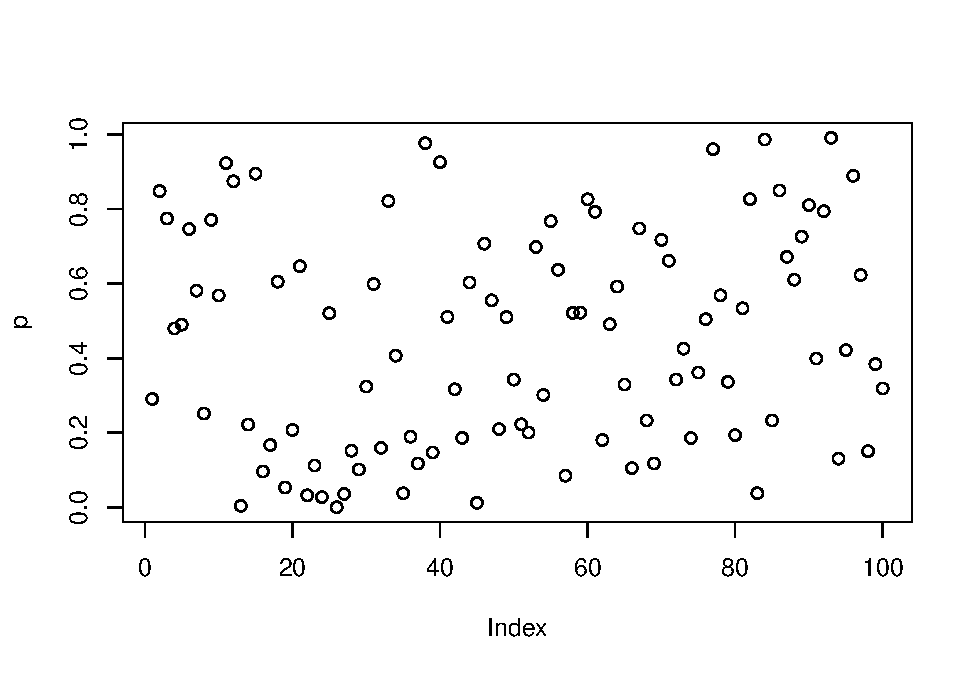
\includegraphics{Functionals_files/figure-latex/unnamed-chunk-10-1.pdf}

\textbf{Q5.} The following code uses a map nested inside another map to apply a function to every element of a nested list. Why does it fail, and what do you need to do to make it work?

\begin{Shaded}
\begin{Highlighting}[]
\NormalTok{x }\OtherTok{\textless{}{-}} \FunctionTok{list}\NormalTok{(}
  \FunctionTok{list}\NormalTok{(}\DecValTok{1}\NormalTok{, }\FunctionTok{c}\NormalTok{(}\DecValTok{3}\NormalTok{, }\DecValTok{9}\NormalTok{)),}
  \FunctionTok{list}\NormalTok{(}\FunctionTok{c}\NormalTok{(}\DecValTok{3}\NormalTok{, }\DecValTok{6}\NormalTok{), }\DecValTok{7}\NormalTok{, }\FunctionTok{c}\NormalTok{(}\DecValTok{4}\NormalTok{, }\DecValTok{7}\NormalTok{, }\DecValTok{6}\NormalTok{))}
\NormalTok{)}

\NormalTok{triple }\OtherTok{\textless{}{-}} \ControlFlowTok{function}\NormalTok{(x) x }\SpecialCharTok{*} \DecValTok{3}
\FunctionTok{map}\NormalTok{(x, map, }\AttributeTok{.f =}\NormalTok{ triple)}
\CommentTok{\#\textgreater{} Error in .f(.x[[i]], ...): unused argument (function (.x, .f, ...) }
\CommentTok{\#\textgreater{} \{}
\CommentTok{\#\textgreater{}     .f \textless{}{-} as\_mapper(.f, ...)}
\CommentTok{\#\textgreater{}     .Call(map\_impl, environment(), ".x", ".f", "list")}
\CommentTok{\#\textgreater{} \})}
\end{Highlighting}
\end{Shaded}

\textbf{A5.} Here is the fixed version:

\begin{Shaded}
\begin{Highlighting}[]
\NormalTok{x }\OtherTok{\textless{}{-}} \FunctionTok{list}\NormalTok{(}
  \FunctionTok{list}\NormalTok{(}\DecValTok{1}\NormalTok{, }\FunctionTok{c}\NormalTok{(}\DecValTok{3}\NormalTok{, }\DecValTok{9}\NormalTok{)),}
  \FunctionTok{list}\NormalTok{(}\FunctionTok{c}\NormalTok{(}\DecValTok{3}\NormalTok{, }\DecValTok{6}\NormalTok{), }\DecValTok{7}\NormalTok{, }\FunctionTok{c}\NormalTok{(}\DecValTok{4}\NormalTok{, }\DecValTok{7}\NormalTok{, }\DecValTok{6}\NormalTok{))}
\NormalTok{)}

\NormalTok{triple }\OtherTok{\textless{}{-}} \ControlFlowTok{function}\NormalTok{(x) x }\SpecialCharTok{*} \DecValTok{3}
\FunctionTok{map}\NormalTok{(x, }\AttributeTok{.f =} \SpecialCharTok{\textasciitilde{}} \FunctionTok{map}\NormalTok{(., }\SpecialCharTok{\textasciitilde{}} \FunctionTok{triple}\NormalTok{(.)))}
\CommentTok{\#\textgreater{} [[1]]}
\CommentTok{\#\textgreater{} [[1]][[1]]}
\CommentTok{\#\textgreater{} [1] 3}
\CommentTok{\#\textgreater{} }
\CommentTok{\#\textgreater{} [[1]][[2]]}
\CommentTok{\#\textgreater{} [1]  9 27}
\CommentTok{\#\textgreater{} }
\CommentTok{\#\textgreater{} }
\CommentTok{\#\textgreater{} [[2]]}
\CommentTok{\#\textgreater{} [[2]][[1]]}
\CommentTok{\#\textgreater{} [1]  9 18}
\CommentTok{\#\textgreater{} }
\CommentTok{\#\textgreater{} [[2]][[2]]}
\CommentTok{\#\textgreater{} [1] 21}
\CommentTok{\#\textgreater{} }
\CommentTok{\#\textgreater{} [[2]][[3]]}
\CommentTok{\#\textgreater{} [1] 12 21 18}
\end{Highlighting}
\end{Shaded}

\textbf{Q6.} Use \texttt{map()} to fit linear models to the \texttt{mtcars} dataset using the formulas stored in this list:

\begin{Shaded}
\begin{Highlighting}[]
\NormalTok{formulas }\OtherTok{\textless{}{-}} \FunctionTok{list}\NormalTok{(}
\NormalTok{  mpg }\SpecialCharTok{\textasciitilde{}}\NormalTok{ disp,}
\NormalTok{  mpg }\SpecialCharTok{\textasciitilde{}} \FunctionTok{I}\NormalTok{(}\DecValTok{1} \SpecialCharTok{/}\NormalTok{ disp),}
\NormalTok{  mpg }\SpecialCharTok{\textasciitilde{}}\NormalTok{ disp }\SpecialCharTok{+}\NormalTok{ wt,}
\NormalTok{  mpg }\SpecialCharTok{\textasciitilde{}} \FunctionTok{I}\NormalTok{(}\DecValTok{1} \SpecialCharTok{/}\NormalTok{ disp) }\SpecialCharTok{+}\NormalTok{ wt}
\NormalTok{)}
\end{Highlighting}
\end{Shaded}

\textbf{A6.} Fitting linear models to the \texttt{mtcars} dataset using the provided formulas:

\begin{Shaded}
\begin{Highlighting}[]
\NormalTok{formulas }\OtherTok{\textless{}{-}} \FunctionTok{list}\NormalTok{(}
\NormalTok{  mpg }\SpecialCharTok{\textasciitilde{}}\NormalTok{ disp,}
\NormalTok{  mpg }\SpecialCharTok{\textasciitilde{}} \FunctionTok{I}\NormalTok{(}\DecValTok{1} \SpecialCharTok{/}\NormalTok{ disp),}
\NormalTok{  mpg }\SpecialCharTok{\textasciitilde{}}\NormalTok{ disp }\SpecialCharTok{+}\NormalTok{ wt,}
\NormalTok{  mpg }\SpecialCharTok{\textasciitilde{}} \FunctionTok{I}\NormalTok{(}\DecValTok{1} \SpecialCharTok{/}\NormalTok{ disp) }\SpecialCharTok{+}\NormalTok{ wt}
\NormalTok{)}

\FunctionTok{map}\NormalTok{(formulas, }\SpecialCharTok{\textasciitilde{}} \FunctionTok{lm}\NormalTok{(}\AttributeTok{formula =}\NormalTok{ ., }\AttributeTok{data =}\NormalTok{ mtcars))}
\CommentTok{\#\textgreater{} [[1]]}
\CommentTok{\#\textgreater{} }
\CommentTok{\#\textgreater{} Call:}
\CommentTok{\#\textgreater{} lm(formula = ., data = mtcars)}
\CommentTok{\#\textgreater{} }
\CommentTok{\#\textgreater{} Coefficients:}
\CommentTok{\#\textgreater{} (Intercept)         disp  }
\CommentTok{\#\textgreater{}    29.59985     {-}0.04122  }
\CommentTok{\#\textgreater{} }
\CommentTok{\#\textgreater{} }
\CommentTok{\#\textgreater{} [[2]]}
\CommentTok{\#\textgreater{} }
\CommentTok{\#\textgreater{} Call:}
\CommentTok{\#\textgreater{} lm(formula = ., data = mtcars)}
\CommentTok{\#\textgreater{} }
\CommentTok{\#\textgreater{} Coefficients:}
\CommentTok{\#\textgreater{} (Intercept)    I(1/disp)  }
\CommentTok{\#\textgreater{}       10.75      1557.67  }
\CommentTok{\#\textgreater{} }
\CommentTok{\#\textgreater{} }
\CommentTok{\#\textgreater{} [[3]]}
\CommentTok{\#\textgreater{} }
\CommentTok{\#\textgreater{} Call:}
\CommentTok{\#\textgreater{} lm(formula = ., data = mtcars)}
\CommentTok{\#\textgreater{} }
\CommentTok{\#\textgreater{} Coefficients:}
\CommentTok{\#\textgreater{} (Intercept)         disp           wt  }
\CommentTok{\#\textgreater{}    34.96055     {-}0.01772     {-}3.35083  }
\CommentTok{\#\textgreater{} }
\CommentTok{\#\textgreater{} }
\CommentTok{\#\textgreater{} [[4]]}
\CommentTok{\#\textgreater{} }
\CommentTok{\#\textgreater{} Call:}
\CommentTok{\#\textgreater{} lm(formula = ., data = mtcars)}
\CommentTok{\#\textgreater{} }
\CommentTok{\#\textgreater{} Coefficients:}
\CommentTok{\#\textgreater{} (Intercept)    I(1/disp)           wt  }
\CommentTok{\#\textgreater{}      19.024     1142.560       {-}1.798}
\end{Highlighting}
\end{Shaded}

\textbf{Q7.} Fit the model \texttt{mpg\ \textasciitilde{}\ disp} to each of the bootstrap replicates of \texttt{mtcars} in the list below, then extract the \(R^2\) of the model fit (Hint: you can compute the \(R^2\) with \texttt{summary()}.)

\begin{Shaded}
\begin{Highlighting}[]
\NormalTok{bootstrap }\OtherTok{\textless{}{-}} \ControlFlowTok{function}\NormalTok{(df) \{}
\NormalTok{  df[}\FunctionTok{sample}\NormalTok{(}\FunctionTok{nrow}\NormalTok{(df), }\AttributeTok{replace =} \ConstantTok{TRUE}\NormalTok{), , drop }\OtherTok{=} \ConstantTok{FALSE}\NormalTok{]}
\NormalTok{\}}

\NormalTok{bootstraps }\OtherTok{\textless{}{-}} \FunctionTok{map}\NormalTok{(}\DecValTok{1}\SpecialCharTok{:}\DecValTok{10}\NormalTok{, }\SpecialCharTok{\textasciitilde{}} \FunctionTok{bootstrap}\NormalTok{(mtcars))}
\end{Highlighting}
\end{Shaded}

\textbf{A7.} This can be done using \texttt{map\_dbl()}:

\begin{Shaded}
\begin{Highlighting}[]
\NormalTok{bootstrap }\OtherTok{\textless{}{-}} \ControlFlowTok{function}\NormalTok{(df) \{}
\NormalTok{  df[}\FunctionTok{sample}\NormalTok{(}\FunctionTok{nrow}\NormalTok{(df), }\AttributeTok{replace =} \ConstantTok{TRUE}\NormalTok{), , drop }\OtherTok{=} \ConstantTok{FALSE}\NormalTok{]}
\NormalTok{\}}

\NormalTok{bootstraps }\OtherTok{\textless{}{-}} \FunctionTok{map}\NormalTok{(}\DecValTok{1}\SpecialCharTok{:}\DecValTok{10}\NormalTok{, }\SpecialCharTok{\textasciitilde{}} \FunctionTok{bootstrap}\NormalTok{(mtcars))}

\FunctionTok{map\_dbl}\NormalTok{(}
\NormalTok{  bootstraps,}
  \SpecialCharTok{\textasciitilde{}} \FunctionTok{summary}\NormalTok{(}\FunctionTok{lm}\NormalTok{(}\AttributeTok{formula =}\NormalTok{ mpg }\SpecialCharTok{\textasciitilde{}}\NormalTok{ disp, }\AttributeTok{data =}\NormalTok{ .))}\SpecialCharTok{$}\NormalTok{r.squared}
\NormalTok{)}
\CommentTok{\#\textgreater{}  [1] 0.6980447 0.7153403 0.6408987 0.7627210 0.6908151}
\CommentTok{\#\textgreater{}  [6] 0.8170847 0.7867446 0.7288730 0.6950510 0.8300409}
\end{Highlighting}
\end{Shaded}

\hypertarget{exercise-9.4.6}{%
\section{Exercise 9.4.6}\label{exercise-9.4.6}}

\textbf{Q1.} Explain the results of \texttt{modify(mtcars,\ 1)}.

\textbf{A1.} \texttt{modify()} returns the object of type same as the input. Since the input here is a data frame of certain dimensions and \texttt{.f\ =\ 1} translates to plucking the first element in each column, it returns a data frames with the same dimensions with the plucked element recycled across rows.

\begin{Shaded}
\begin{Highlighting}[]
\FunctionTok{head}\NormalTok{(}\FunctionTok{modify}\NormalTok{(mtcars, }\DecValTok{1}\NormalTok{))}
\CommentTok{\#\textgreater{}                   mpg cyl disp  hp drat   wt  qsec vs am}
\CommentTok{\#\textgreater{} Mazda RX4          21   6  160 110  3.9 2.62 16.46  0  1}
\CommentTok{\#\textgreater{} Mazda RX4 Wag      21   6  160 110  3.9 2.62 16.46  0  1}
\CommentTok{\#\textgreater{} Datsun 710         21   6  160 110  3.9 2.62 16.46  0  1}
\CommentTok{\#\textgreater{} Hornet 4 Drive     21   6  160 110  3.9 2.62 16.46  0  1}
\CommentTok{\#\textgreater{} Hornet Sportabout  21   6  160 110  3.9 2.62 16.46  0  1}
\CommentTok{\#\textgreater{} Valiant            21   6  160 110  3.9 2.62 16.46  0  1}
\CommentTok{\#\textgreater{}                   gear carb}
\CommentTok{\#\textgreater{} Mazda RX4            4    4}
\CommentTok{\#\textgreater{} Mazda RX4 Wag        4    4}
\CommentTok{\#\textgreater{} Datsun 710           4    4}
\CommentTok{\#\textgreater{} Hornet 4 Drive       4    4}
\CommentTok{\#\textgreater{} Hornet Sportabout    4    4}
\CommentTok{\#\textgreater{} Valiant              4    4}
\end{Highlighting}
\end{Shaded}

\textbf{Q2.} Rewrite the following code to use \texttt{iwalk()} instead of \texttt{walk2()}. What are the advantages and disadvantages?

\begin{Shaded}
\begin{Highlighting}[]
\NormalTok{cyls }\OtherTok{\textless{}{-}} \FunctionTok{split}\NormalTok{(mtcars, mtcars}\SpecialCharTok{$}\NormalTok{cyl)}
\NormalTok{paths }\OtherTok{\textless{}{-}} \FunctionTok{file.path}\NormalTok{(temp, }\FunctionTok{paste0}\NormalTok{(}\StringTok{"cyl{-}"}\NormalTok{, }\FunctionTok{names}\NormalTok{(cyls), }\StringTok{".csv"}\NormalTok{))}
\FunctionTok{walk2}\NormalTok{(cyls, paths, write.csv)}
\end{Highlighting}
\end{Shaded}

\textbf{A2.} Rewritten versions are below:

\begin{itemize}
\tightlist
\item
  with \texttt{walk2()}
\end{itemize}

\begin{Shaded}
\begin{Highlighting}[]
\NormalTok{cyls }\OtherTok{\textless{}{-}} \FunctionTok{split}\NormalTok{(mtcars, mtcars}\SpecialCharTok{$}\NormalTok{cyl)}
\NormalTok{paths }\OtherTok{\textless{}{-}} \FunctionTok{file.path}\NormalTok{(temp, }\FunctionTok{paste0}\NormalTok{(}\StringTok{"cyl{-}"}\NormalTok{, }\FunctionTok{names}\NormalTok{(cyls), }\StringTok{".csv"}\NormalTok{))}
\FunctionTok{walk2}\NormalTok{(}\AttributeTok{.x =}\NormalTok{ cyls, }\AttributeTok{.y =}\NormalTok{ paths, }\AttributeTok{.f =}\NormalTok{ write.csv)}
\end{Highlighting}
\end{Shaded}

\begin{itemize}
\tightlist
\item
  with \texttt{iwalk()}
\end{itemize}

\begin{Shaded}
\begin{Highlighting}[]
\NormalTok{cyls }\OtherTok{\textless{}{-}} \FunctionTok{split}\NormalTok{(mtcars, mtcars}\SpecialCharTok{$}\NormalTok{cyl)}
\FunctionTok{names}\NormalTok{(cyls) }\OtherTok{\textless{}{-}} \FunctionTok{file.path}\NormalTok{(temp, }\FunctionTok{paste0}\NormalTok{(}\StringTok{"cyl{-}"}\NormalTok{, }\FunctionTok{names}\NormalTok{(cyls), }\StringTok{".csv"}\NormalTok{))}
\FunctionTok{iwalk}\NormalTok{(cyls, }\SpecialCharTok{\textasciitilde{}} \FunctionTok{write.csv}\NormalTok{(.x, .y))}
\end{Highlighting}
\end{Shaded}

\textbf{Q3.} Explain how the following code transforms a data frame using functions stored in a list.

\begin{Shaded}
\begin{Highlighting}[]
\NormalTok{trans }\OtherTok{\textless{}{-}} \FunctionTok{list}\NormalTok{(}
  \AttributeTok{disp =} \ControlFlowTok{function}\NormalTok{(x) x }\SpecialCharTok{*} \FloatTok{0.0163871}\NormalTok{,}
  \AttributeTok{am =} \ControlFlowTok{function}\NormalTok{(x) }\FunctionTok{factor}\NormalTok{(x, }\AttributeTok{labels =} \FunctionTok{c}\NormalTok{(}\StringTok{"auto"}\NormalTok{, }\StringTok{"manual"}\NormalTok{))}
\NormalTok{)}

\NormalTok{nm }\OtherTok{\textless{}{-}} \FunctionTok{names}\NormalTok{(trans)}
\NormalTok{mtcars[nm] }\OtherTok{\textless{}{-}} \FunctionTok{map2}\NormalTok{(trans, mtcars[nm], }\ControlFlowTok{function}\NormalTok{(f, var) }\FunctionTok{f}\NormalTok{(var))}
\end{Highlighting}
\end{Shaded}

Compare and contrast the \texttt{map2()} approach to this \texttt{map()} approach:

\begin{Shaded}
\begin{Highlighting}[]
\NormalTok{mtcars[nm] }\OtherTok{\textless{}{-}} \FunctionTok{map}\NormalTok{(nm, }\SpecialCharTok{\textasciitilde{}}\NormalTok{ trans[[.x]](mtcars[[.x]]))}
\end{Highlighting}
\end{Shaded}

\textbf{A3.} \texttt{map2()} supplies the functions defined in \texttt{.x\ =\ trans} as \texttt{f} in the anonymous functions, while the names of the columns defined in \texttt{.y\ =\ mtcars{[}nm{]}} are picked up by \texttt{var} in the anonymous function. Note that the function is iterating over indices for vectors of transformations and column names.

\begin{Shaded}
\begin{Highlighting}[]
\NormalTok{trans }\OtherTok{\textless{}{-}} \FunctionTok{list}\NormalTok{(}
  \AttributeTok{disp =} \ControlFlowTok{function}\NormalTok{(x) x }\SpecialCharTok{*} \FloatTok{0.0163871}\NormalTok{,}
  \AttributeTok{am =} \ControlFlowTok{function}\NormalTok{(x) }\FunctionTok{factor}\NormalTok{(x, }\AttributeTok{labels =} \FunctionTok{c}\NormalTok{(}\StringTok{"auto"}\NormalTok{, }\StringTok{"manual"}\NormalTok{))}
\NormalTok{)}

\NormalTok{nm }\OtherTok{\textless{}{-}} \FunctionTok{names}\NormalTok{(trans)}
\NormalTok{mtcars[nm] }\OtherTok{\textless{}{-}} \FunctionTok{map2}\NormalTok{(trans, mtcars[nm], }\ControlFlowTok{function}\NormalTok{(f, var) }\FunctionTok{f}\NormalTok{(var))}
\end{Highlighting}
\end{Shaded}

In the \texttt{map()} approach, the function is iterating over indices for vectors of column names.

\begin{Shaded}
\begin{Highlighting}[]
\NormalTok{mtcars[nm] }\OtherTok{\textless{}{-}} \FunctionTok{map}\NormalTok{(nm, }\SpecialCharTok{\textasciitilde{}}\NormalTok{ trans[[.x]](mtcars[[.x]]))}
\end{Highlighting}
\end{Shaded}

\textbf{Q4.} What does \texttt{write.csv()} return, i.e.~what happens if you use it with \texttt{map2()} instead of \texttt{walk2()}?

\textbf{A4.} If we use \texttt{map2()}, it will work, but it will print \texttt{NULL}s to the terminal for every list element.

\begin{Shaded}
\begin{Highlighting}[]
\NormalTok{bods }\OtherTok{\textless{}{-}} \FunctionTok{split}\NormalTok{(BOD, BOD}\SpecialCharTok{$}\NormalTok{Time)}
\NormalTok{nm }\OtherTok{\textless{}{-}} \FunctionTok{names}\NormalTok{(bods)}
\FunctionTok{map2}\NormalTok{(bods, nm, write.csv)}
\end{Highlighting}
\end{Shaded}

\hypertarget{exercise-9.6.3}{%
\section{Exercise 9.6.3}\label{exercise-9.6.3}}

\textbf{Q1.} Why isn't \texttt{is.na()} a predicate function? What base R function is closest to being a predicate version of \texttt{is.na()}?

\textbf{A1.} As mentioned in the docs:

\begin{quote}
A predicate is a function that returns a \textbf{single} \texttt{TRUE} or \texttt{FALSE}.
\end{quote}

The \texttt{is.na()} function does not return a \texttt{logical} scalar, but instead returns a vector and thus isn't a predicate function.

\begin{Shaded}
\begin{Highlighting}[]
\CommentTok{\# contrast the following behavior of predicate functions}
\FunctionTok{is.character}\NormalTok{(}\FunctionTok{c}\NormalTok{(}\StringTok{"x"}\NormalTok{, }\DecValTok{2}\NormalTok{))}
\CommentTok{\#\textgreater{} [1] TRUE}
\FunctionTok{is.null}\NormalTok{(}\FunctionTok{c}\NormalTok{(}\DecValTok{3}\NormalTok{, }\ConstantTok{NULL}\NormalTok{))}
\CommentTok{\#\textgreater{} [1] FALSE}

\CommentTok{\# with this behavior}
\FunctionTok{is.na}\NormalTok{(}\FunctionTok{c}\NormalTok{(}\ConstantTok{NA}\NormalTok{, }\DecValTok{1}\NormalTok{))}
\CommentTok{\#\textgreater{} [1]  TRUE FALSE}
\end{Highlighting}
\end{Shaded}

The closest equivalent of a predicate function in base-R is \texttt{anyNA()} function.

\begin{Shaded}
\begin{Highlighting}[]
\FunctionTok{anyNA}\NormalTok{(}\FunctionTok{c}\NormalTok{(}\ConstantTok{NA}\NormalTok{, }\DecValTok{1}\NormalTok{))}
\CommentTok{\#\textgreater{} [1] TRUE}
\end{Highlighting}
\end{Shaded}

\textbf{Q2.} \texttt{simple\_reduce()} has a problem when \texttt{x} is length 0 or length 1. Describe the source of the problem and how you might go about fixing it.

\begin{Shaded}
\begin{Highlighting}[]
\NormalTok{simple\_reduce }\OtherTok{\textless{}{-}} \ControlFlowTok{function}\NormalTok{(x, f) \{}
\NormalTok{  out }\OtherTok{\textless{}{-}}\NormalTok{ x[[}\DecValTok{1}\NormalTok{]]}
  \ControlFlowTok{for}\NormalTok{ (i }\ControlFlowTok{in} \FunctionTok{seq}\NormalTok{(}\DecValTok{2}\NormalTok{, }\FunctionTok{length}\NormalTok{(x))) \{}
\NormalTok{    out }\OtherTok{\textless{}{-}} \FunctionTok{f}\NormalTok{(out, x[[i]])}
\NormalTok{  \}}
\NormalTok{  out}
\NormalTok{\}}
\end{Highlighting}
\end{Shaded}

\textbf{A2.} Supplied function:

\begin{Shaded}
\begin{Highlighting}[]
\NormalTok{simple\_reduce }\OtherTok{\textless{}{-}} \ControlFlowTok{function}\NormalTok{(x, f) \{}
\NormalTok{  out }\OtherTok{\textless{}{-}}\NormalTok{ x[[}\DecValTok{1}\NormalTok{]]}
  \ControlFlowTok{for}\NormalTok{ (i }\ControlFlowTok{in} \FunctionTok{seq}\NormalTok{(}\DecValTok{2}\NormalTok{, }\FunctionTok{length}\NormalTok{(x))) \{}
\NormalTok{    out }\OtherTok{\textless{}{-}} \FunctionTok{f}\NormalTok{(out, x[[i]])}
\NormalTok{  \}}
\NormalTok{  out}
\NormalTok{\}}
\end{Highlighting}
\end{Shaded}

This function struggles with inputs of length 0 and 1 because function tries to access out-of-bound values.

\begin{Shaded}
\begin{Highlighting}[]
\FunctionTok{simple\_reduce}\NormalTok{(}\FunctionTok{numeric}\NormalTok{(), sum)}
\CommentTok{\#\textgreater{} Error in x[[1]]: subscript out of bounds}
\FunctionTok{simple\_reduce}\NormalTok{(}\DecValTok{1}\NormalTok{, sum)}
\CommentTok{\#\textgreater{} Error in x[[i]]: subscript out of bounds}
\FunctionTok{simple\_reduce}\NormalTok{(}\DecValTok{1}\SpecialCharTok{:}\DecValTok{3}\NormalTok{, sum)}
\CommentTok{\#\textgreater{} [1] 6}
\end{Highlighting}
\end{Shaded}

This problem can be solved by adding \texttt{init} argument, which supplies the default or initial value for the function to operate on:

\begin{Shaded}
\begin{Highlighting}[]
\NormalTok{simple\_reduce2 }\OtherTok{\textless{}{-}} \ControlFlowTok{function}\NormalTok{(x, f, }\AttributeTok{init =} \DecValTok{0}\NormalTok{) \{}
  \CommentTok{\# initializer will become the first value}
  \ControlFlowTok{if}\NormalTok{ (}\FunctionTok{length}\NormalTok{(x) }\SpecialCharTok{==}\NormalTok{ 0L) \{}
    \FunctionTok{return}\NormalTok{(init)}
\NormalTok{  \}}

  \ControlFlowTok{if}\NormalTok{ (}\FunctionTok{length}\NormalTok{(x) }\SpecialCharTok{==}\NormalTok{ 1L) \{}
    \FunctionTok{return}\NormalTok{(x[[1L]])}
\NormalTok{  \}}

\NormalTok{  out }\OtherTok{\textless{}{-}}\NormalTok{ x[[}\DecValTok{1}\NormalTok{]]}

  \ControlFlowTok{for}\NormalTok{ (i }\ControlFlowTok{in} \FunctionTok{seq}\NormalTok{(}\DecValTok{2}\NormalTok{, }\FunctionTok{length}\NormalTok{(x))) \{}
\NormalTok{    out }\OtherTok{\textless{}{-}} \FunctionTok{f}\NormalTok{(out, x[[i]])}
\NormalTok{  \}}
\NormalTok{  out}
\NormalTok{\}}
\end{Highlighting}
\end{Shaded}

Let's try it out:

\begin{Shaded}
\begin{Highlighting}[]
\FunctionTok{simple\_reduce2}\NormalTok{(}\FunctionTok{numeric}\NormalTok{(), sum)}
\CommentTok{\#\textgreater{} [1] 0}
\FunctionTok{simple\_reduce2}\NormalTok{(}\DecValTok{1}\NormalTok{, sum)}
\CommentTok{\#\textgreater{} [1] 1}
\FunctionTok{simple\_reduce2}\NormalTok{(}\DecValTok{1}\SpecialCharTok{:}\DecValTok{3}\NormalTok{, sum)}
\CommentTok{\#\textgreater{} [1] 6}
\end{Highlighting}
\end{Shaded}

With a different kind of function:

\begin{Shaded}
\begin{Highlighting}[]
\FunctionTok{simple\_reduce2}\NormalTok{(}\FunctionTok{numeric}\NormalTok{(), }\StringTok{\textasciigrave{}}\AttributeTok{*}\StringTok{\textasciigrave{}}\NormalTok{, }\AttributeTok{init =} \DecValTok{1}\NormalTok{)}
\CommentTok{\#\textgreater{} [1] 1}
\FunctionTok{simple\_reduce2}\NormalTok{(}\DecValTok{1}\NormalTok{, }\StringTok{\textasciigrave{}}\AttributeTok{*}\StringTok{\textasciigrave{}}\NormalTok{, }\AttributeTok{init =} \DecValTok{1}\NormalTok{)}
\CommentTok{\#\textgreater{} [1] 1}
\FunctionTok{simple\_reduce2}\NormalTok{(}\DecValTok{1}\SpecialCharTok{:}\DecValTok{3}\NormalTok{, }\StringTok{\textasciigrave{}}\AttributeTok{*}\StringTok{\textasciigrave{}}\NormalTok{, }\AttributeTok{init =} \DecValTok{1}\NormalTok{)}
\CommentTok{\#\textgreater{} [1] 6}
\end{Highlighting}
\end{Shaded}

And another one:

\begin{Shaded}
\begin{Highlighting}[]
\FunctionTok{simple\_reduce2}\NormalTok{(}\FunctionTok{numeric}\NormalTok{(), }\StringTok{\textasciigrave{}}\AttributeTok{\%/\%}\StringTok{\textasciigrave{}}\NormalTok{)}
\CommentTok{\#\textgreater{} [1] 0}
\FunctionTok{simple\_reduce2}\NormalTok{(}\DecValTok{1}\NormalTok{, }\StringTok{\textasciigrave{}}\AttributeTok{\%/\%}\StringTok{\textasciigrave{}}\NormalTok{)}
\CommentTok{\#\textgreater{} [1] 1}
\FunctionTok{simple\_reduce2}\NormalTok{(}\DecValTok{1}\SpecialCharTok{:}\DecValTok{3}\NormalTok{, }\StringTok{\textasciigrave{}}\AttributeTok{\%/\%}\StringTok{\textasciigrave{}}\NormalTok{)}
\CommentTok{\#\textgreater{} [1] 0}
\end{Highlighting}
\end{Shaded}

\textbf{Q3.} Implement the \texttt{span()} function from Haskell: given a list \texttt{x} and a predicate function \texttt{f}, \texttt{span(x,\ f)} returns the location of the longest sequential run of elements where the predicate is true. (Hint: you might find \texttt{rle()} helpful.)

\textbf{Q4.} Implement \texttt{arg\_max()}. It should take a function and a vector of inputs, and return the elements of the input where the function returns the highest value. For example, \texttt{arg\_max(-10:5,\ function(x)\ x\ \^{}\ 2)} should return -10. \texttt{arg\_max(-5:5,\ function(x)\ x\ \^{}\ 2)} should return \texttt{c(-5,\ 5)}. Also implement the matching \texttt{arg\_min()} function.

\textbf{Q5.} The function below scales a vector so it falls in the range {[}0, 1{]}. How would you apply it to every column of a data frame? How would you apply it to every numeric column in a data frame?

\begin{Shaded}
\begin{Highlighting}[]
\NormalTok{scale01 }\OtherTok{\textless{}{-}} \ControlFlowTok{function}\NormalTok{(x) \{}
\NormalTok{  rng }\OtherTok{\textless{}{-}} \FunctionTok{range}\NormalTok{(x, }\AttributeTok{na.rm =} \ConstantTok{TRUE}\NormalTok{)}
\NormalTok{  (x }\SpecialCharTok{{-}}\NormalTok{ rng[}\DecValTok{1}\NormalTok{]) }\SpecialCharTok{/}\NormalTok{ (rng[}\DecValTok{2}\NormalTok{] }\SpecialCharTok{{-}}\NormalTok{ rng[}\DecValTok{1}\NormalTok{])}
\NormalTok{\}}
\end{Highlighting}
\end{Shaded}

\hypertarget{exercise-9.7.3}{%
\section{Exercise 9.7.3}\label{exercise-9.7.3}}

\textbf{Q1.} How does \texttt{apply()} arrange the output? Read the documentation and perform some experiments.

\textbf{Q2.} What do \texttt{eapply()} and \texttt{rapply()} do? Does purrr have equivalents?

\textbf{A2.} As mentioned in the documentation:

\begin{itemize}
\tightlist
\item
  \texttt{eapply()}
\end{itemize}

\begin{quote}
\texttt{eapply()} applies FUN to the named values from an environment and returns the results as a list.
\end{quote}

Here is an example:

\begin{Shaded}
\begin{Highlighting}[]
\FunctionTok{library}\NormalTok{(rlang)}
\CommentTok{\#\textgreater{} }
\CommentTok{\#\textgreater{} Attaching package: \textquotesingle{}rlang\textquotesingle{}}
\CommentTok{\#\textgreater{} The following objects are masked from \textquotesingle{}package:purrr\textquotesingle{}:}
\CommentTok{\#\textgreater{} }
\CommentTok{\#\textgreater{}     \%@\%, as\_function, flatten, flatten\_chr,}
\CommentTok{\#\textgreater{}     flatten\_dbl, flatten\_int, flatten\_lgl,}
\CommentTok{\#\textgreater{}     flatten\_raw, invoke, splice}

\NormalTok{e }\OtherTok{\textless{}{-}} \FunctionTok{env}\NormalTok{(}\StringTok{"x"} \OtherTok{=} \DecValTok{1}\NormalTok{, }\StringTok{"y"} \OtherTok{=} \DecValTok{2}\NormalTok{)}
\NormalTok{rlang}\SpecialCharTok{::}\FunctionTok{env\_print}\NormalTok{(e)}
\CommentTok{\#\textgreater{} \textless{}environment: 0x106ba6518\textgreater{}}
\CommentTok{\#\textgreater{} Parent: \textless{}environment: global\textgreater{}}
\CommentTok{\#\textgreater{} Bindings:}
\CommentTok{\#\textgreater{} * x: \textless{}dbl\textgreater{}}
\CommentTok{\#\textgreater{} * y: \textless{}dbl\textgreater{}}

\FunctionTok{eapply}\NormalTok{(e, as.character)}
\CommentTok{\#\textgreater{} $x}
\CommentTok{\#\textgreater{} [1] "1"}
\CommentTok{\#\textgreater{} }
\CommentTok{\#\textgreater{} $y}
\CommentTok{\#\textgreater{} [1] "2"}
\end{Highlighting}
\end{Shaded}

\texttt{\{purrr\}} doesn't have any function to iterate over environments.

\begin{itemize}
\tightlist
\item
  \texttt{rapply()}
\end{itemize}

\begin{quote}
\texttt{rapply()} is a recursive version of lapply with flexibility in how the result is structured (how = ``..'').
\end{quote}

Here is an example:

\begin{Shaded}
\begin{Highlighting}[]
\NormalTok{X }\OtherTok{\textless{}{-}} \FunctionTok{list}\NormalTok{(}\FunctionTok{list}\NormalTok{(}\AttributeTok{a =} \ConstantTok{TRUE}\NormalTok{, }\AttributeTok{b =} \FunctionTok{list}\NormalTok{(}\AttributeTok{c =} \FunctionTok{c}\NormalTok{(4L, }\FloatTok{3.2}\NormalTok{))), }\AttributeTok{d =} \FloatTok{9.0}\NormalTok{)}

\FunctionTok{rapply}\NormalTok{(X, as.character, }\AttributeTok{classes =} \StringTok{"numeric"}\NormalTok{, }\AttributeTok{how =} \StringTok{"replace"}\NormalTok{)}
\CommentTok{\#\textgreater{} [[1]]}
\CommentTok{\#\textgreater{} [[1]]$a}
\CommentTok{\#\textgreater{} [1] TRUE}
\CommentTok{\#\textgreater{} }
\CommentTok{\#\textgreater{} [[1]]$b}
\CommentTok{\#\textgreater{} [[1]]$b$c}
\CommentTok{\#\textgreater{} [1] "4"   "3.2"}
\CommentTok{\#\textgreater{} }
\CommentTok{\#\textgreater{} }
\CommentTok{\#\textgreater{} }
\CommentTok{\#\textgreater{} $d}
\CommentTok{\#\textgreater{} [1] "9"}
\end{Highlighting}
\end{Shaded}

\texttt{\{purrr\}} has something similar in \texttt{modify\_depth()}.

\begin{Shaded}
\begin{Highlighting}[]
\NormalTok{X }\OtherTok{\textless{}{-}} \FunctionTok{list}\NormalTok{(}\FunctionTok{list}\NormalTok{(}\AttributeTok{a =} \ConstantTok{TRUE}\NormalTok{, }\AttributeTok{b =} \FunctionTok{list}\NormalTok{(}\AttributeTok{c =} \FunctionTok{c}\NormalTok{(4L, }\FloatTok{3.2}\NormalTok{))), }\AttributeTok{d =} \FloatTok{9.0}\NormalTok{)}

\NormalTok{purrr}\SpecialCharTok{::}\FunctionTok{modify\_depth}\NormalTok{(X, }\AttributeTok{.depth =}\NormalTok{ 2L, }\AttributeTok{.f =}\NormalTok{ length)}
\CommentTok{\#\textgreater{} [[1]]}
\CommentTok{\#\textgreater{} [[1]]$a}
\CommentTok{\#\textgreater{} [1] 1}
\CommentTok{\#\textgreater{} }
\CommentTok{\#\textgreater{} [[1]]$b}
\CommentTok{\#\textgreater{} [1] 1}
\CommentTok{\#\textgreater{} }
\CommentTok{\#\textgreater{} }
\CommentTok{\#\textgreater{} $d}
\CommentTok{\#\textgreater{} [1] 1}
\end{Highlighting}
\end{Shaded}

\textbf{Q3.} Challenge: read about the \href{https://mitpress.mit.edu/sites/default/files/sicp/full-text/book/book-Z-H-12.html\#\%25_idx_1096}{fixed point algorithm}. Complete the exercises using R.

\hypertarget{function-factories}{%
\chapter{Function factories}\label{function-factories}}

\hypertarget{base-types}{%
\chapter{Base Types}\label{base-types}}

No exercises.

\hypertarget{s3}{%
\chapter{S3}\label{s3}}

\hypertarget{exercise-13.2.1}{%
\section{Exercise 13.2.1}\label{exercise-13.2.1}}

\textbf{Q1.} Describe the difference between \texttt{t.test()} and \texttt{t.data.frame()}. When is each function called?

\textbf{A1.}

\begin{itemize}
\item
  \texttt{t.test()} is a \textbf{generic} function to perform a \emph{t}-test.
\item
  \texttt{t.data.frame} is a \textbf{method} for generic \texttt{t()} (a matrix transform function) and will be dispatched for \texttt{data.frame} class objects/instances that need to be transformed.
\end{itemize}

\begin{Shaded}
\begin{Highlighting}[]
\FunctionTok{library}\NormalTok{(sloop)}

\CommentTok{\# function type}
\FunctionTok{ftype}\NormalTok{(t.test)}
\CommentTok{\#\textgreater{} [1] "S3"      "generic"}
\FunctionTok{ftype}\NormalTok{(t.data.frame)}
\CommentTok{\#\textgreater{} [1] "S3"     "method"}
\end{Highlighting}
\end{Shaded}

\textbf{Q2.} Make a list of commonly used base R functions that contain \texttt{.} in their name but are not \texttt{S3} methods.

\textbf{A2.} Here are a few common R functions with \texttt{.} but that are not \texttt{S3} methods:

\begin{itemize}
\tightlist
\item
  \texttt{all.equal()}
\item
  Most of \texttt{as.*} functions (like \texttt{as.data.frame()}, \texttt{as.numeric()}, etc.)
\item
  \texttt{install.packages()}
\item
  \texttt{on.exit()}
  etc.
\end{itemize}

For full list, you could do:

\begin{Shaded}
\begin{Highlighting}[]
\NormalTok{base\_functions }\OtherTok{\textless{}{-}} \FunctionTok{getNamespaceExports}\NormalTok{(}\StringTok{"base"}\NormalTok{)}

\NormalTok{base\_functions[}\FunctionTok{grepl}\NormalTok{(}\StringTok{"(}\SpecialCharTok{\textbackslash{}\textbackslash{}}\StringTok{w+)(}\SpecialCharTok{\textbackslash{}\textbackslash{}}\StringTok{.)(}\SpecialCharTok{\textbackslash{}\textbackslash{}}\StringTok{w+)"}\NormalTok{, base\_functions)]}
\end{Highlighting}
\end{Shaded}

For example,

\begin{Shaded}
\begin{Highlighting}[]
\FunctionTok{ftype}\NormalTok{(as.data.frame)}
\CommentTok{\#\textgreater{} [1] "S3"      "generic"}
\FunctionTok{ftype}\NormalTok{(on.exit)}
\CommentTok{\#\textgreater{} [1] "primitive"}
\end{Highlighting}
\end{Shaded}

\textbf{Q3.} What does the \texttt{as.data.frame.data.frame()} method do? Why is it confusing? How could you avoid this confusion in your own code?

\textbf{A3.} It's an \texttt{S3} \textbf{method} for \textbf{generic} \texttt{as.data.frame()}.

\begin{Shaded}
\begin{Highlighting}[]
\FunctionTok{ftype}\NormalTok{(as.data.frame.data.frame)}
\CommentTok{\#\textgreater{} [1] "S3"     "method"}
\end{Highlighting}
\end{Shaded}

It can be seen in all methods supported by this generic:

\begin{Shaded}
\begin{Highlighting}[]
\FunctionTok{s3\_methods\_generic}\NormalTok{(}\StringTok{"as.data.frame"}\NormalTok{) }\SpecialCharTok{\%\textgreater{}\%}
\NormalTok{  dplyr}\SpecialCharTok{::}\FunctionTok{filter}\NormalTok{(class }\SpecialCharTok{==} \StringTok{"data.frame"}\NormalTok{)}
\CommentTok{\#\textgreater{} \# A tibble: 1 x 4}
\CommentTok{\#\textgreater{}   generic       class      visible source}
\CommentTok{\#\textgreater{}   \textless{}chr\textgreater{}         \textless{}chr\textgreater{}      \textless{}lgl\textgreater{}   \textless{}chr\textgreater{} }
\CommentTok{\#\textgreater{} 1 as.data.frame data.frame TRUE    base}
\end{Highlighting}
\end{Shaded}

\textbf{Q4.} Describe the difference in behaviour in these two calls.

\begin{Shaded}
\begin{Highlighting}[]
\FunctionTok{set.seed}\NormalTok{(}\DecValTok{1014}\NormalTok{)}
\NormalTok{some\_days }\OtherTok{\textless{}{-}} \FunctionTok{as.Date}\NormalTok{(}\StringTok{"2017{-}01{-}31"}\NormalTok{) }\SpecialCharTok{+} \FunctionTok{sample}\NormalTok{(}\DecValTok{10}\NormalTok{, }\DecValTok{5}\NormalTok{)}
\FunctionTok{mean}\NormalTok{(some\_days)}
\CommentTok{\#\textgreater{} [1] "2017{-}02{-}06"}
\FunctionTok{mean}\NormalTok{(}\FunctionTok{unclass}\NormalTok{(some\_days))}
\CommentTok{\#\textgreater{} [1] 17203.4}
\end{Highlighting}
\end{Shaded}

\textbf{A4.}

\begin{itemize}
\tightlist
\item
  Before unclassing, the \texttt{mean} generic dispatches \texttt{.Date} method:
\end{itemize}

\begin{Shaded}
\begin{Highlighting}[]
\NormalTok{some\_days }\OtherTok{\textless{}{-}} \FunctionTok{as.Date}\NormalTok{(}\StringTok{"2017{-}01{-}31"}\NormalTok{) }\SpecialCharTok{+} \FunctionTok{sample}\NormalTok{(}\DecValTok{10}\NormalTok{, }\DecValTok{5}\NormalTok{)}

\NormalTok{some\_days}
\CommentTok{\#\textgreater{} [1] "2017{-}02{-}06" "2017{-}02{-}09" "2017{-}02{-}05" "2017{-}02{-}08"}
\CommentTok{\#\textgreater{} [5] "2017{-}02{-}07"}

\FunctionTok{s3\_dispatch}\NormalTok{(}\FunctionTok{mean}\NormalTok{(some\_days))}
\CommentTok{\#\textgreater{} =\textgreater{} mean.Date}
\CommentTok{\#\textgreater{}  * mean.default}

\FunctionTok{mean}\NormalTok{(some\_days)}
\CommentTok{\#\textgreater{} [1] "2017{-}02{-}07"}
\end{Highlighting}
\end{Shaded}

\begin{itemize}
\tightlist
\item
  After unclassing, the \texttt{mean} generic dispatches \texttt{.numeric} method:
\end{itemize}

\begin{Shaded}
\begin{Highlighting}[]
\FunctionTok{unclass}\NormalTok{(some\_days)}
\CommentTok{\#\textgreater{} [1] 17203 17206 17202 17205 17204}

\FunctionTok{mean}\NormalTok{(}\FunctionTok{unclass}\NormalTok{(some\_days))}
\CommentTok{\#\textgreater{} [1] 17204}

\FunctionTok{s3\_dispatch}\NormalTok{(}\FunctionTok{mean}\NormalTok{(}\FunctionTok{unclass}\NormalTok{(some\_days)))}
\CommentTok{\#\textgreater{}    mean.double}
\CommentTok{\#\textgreater{}    mean.numeric}
\CommentTok{\#\textgreater{} =\textgreater{} mean.default}
\end{Highlighting}
\end{Shaded}

\textbf{Q5.} What class of object does the following code return? What base type is it built on? What attributes does it use?

\begin{Shaded}
\begin{Highlighting}[]
\NormalTok{x }\OtherTok{\textless{}{-}} \FunctionTok{ecdf}\NormalTok{(}\FunctionTok{rpois}\NormalTok{(}\DecValTok{100}\NormalTok{, }\DecValTok{10}\NormalTok{))}
\NormalTok{x}
\end{Highlighting}
\end{Shaded}

\textbf{A5.} The object is based on base type \texttt{closure}\footnote{of ``object of type `closure' is not subsettable'' fame}, which is a type of function.

\begin{Shaded}
\begin{Highlighting}[]
\NormalTok{x }\OtherTok{\textless{}{-}} \FunctionTok{ecdf}\NormalTok{(}\FunctionTok{rpois}\NormalTok{(}\DecValTok{100}\NormalTok{, }\DecValTok{10}\NormalTok{))}
\NormalTok{x}
\CommentTok{\#\textgreater{} Empirical CDF }
\CommentTok{\#\textgreater{} Call: ecdf(rpois(100, 10))}
\CommentTok{\#\textgreater{}  x[1:18] =      2,      3,      4,  ...,     18,     19}

\FunctionTok{otype}\NormalTok{(x)}
\CommentTok{\#\textgreater{} [1] "S3"}
\FunctionTok{typeof}\NormalTok{(x)}
\CommentTok{\#\textgreater{} [1] "closure"}
\end{Highlighting}
\end{Shaded}

Its class is \texttt{ecdf}, which has other superclasses.

\begin{Shaded}
\begin{Highlighting}[]
\FunctionTok{s3\_class}\NormalTok{(x)}
\CommentTok{\#\textgreater{} [1] "ecdf"     "stepfun"  "function"}
\end{Highlighting}
\end{Shaded}

Apart from \texttt{class}, it has the following attributes:

\begin{Shaded}
\begin{Highlighting}[]
\FunctionTok{attributes}\NormalTok{(x)}
\CommentTok{\#\textgreater{} $class}
\CommentTok{\#\textgreater{} [1] "ecdf"     "stepfun"  "function"}
\CommentTok{\#\textgreater{} }
\CommentTok{\#\textgreater{} $call}
\CommentTok{\#\textgreater{} ecdf(rpois(100, 10))}
\end{Highlighting}
\end{Shaded}

\textbf{Q6.} What class of object does the following code return? What base type is it built on? What attributes does it use?

\begin{Shaded}
\begin{Highlighting}[]
\NormalTok{x }\OtherTok{\textless{}{-}} \FunctionTok{table}\NormalTok{(}\FunctionTok{rpois}\NormalTok{(}\DecValTok{100}\NormalTok{, }\DecValTok{5}\NormalTok{))}
\NormalTok{x}
\end{Highlighting}
\end{Shaded}

\textbf{A6.} The object is based on base type \texttt{integer}.

\begin{Shaded}
\begin{Highlighting}[]
\NormalTok{x }\OtherTok{\textless{}{-}} \FunctionTok{table}\NormalTok{(}\FunctionTok{rpois}\NormalTok{(}\DecValTok{100}\NormalTok{, }\DecValTok{5}\NormalTok{))}
\NormalTok{x}
\CommentTok{\#\textgreater{} }
\CommentTok{\#\textgreater{}  1  2  3  4  5  6  7  8  9 10 }
\CommentTok{\#\textgreater{}  7  7 18 13 14 14 16  4  4  3}

\FunctionTok{otype}\NormalTok{(x)}
\CommentTok{\#\textgreater{} [1] "S3"}
\FunctionTok{typeof}\NormalTok{(x)}
\CommentTok{\#\textgreater{} [1] "integer"}
\end{Highlighting}
\end{Shaded}

Its class is \texttt{table}.

\begin{Shaded}
\begin{Highlighting}[]
\FunctionTok{s3\_class}\NormalTok{(x)}
\CommentTok{\#\textgreater{} [1] "table"}
\end{Highlighting}
\end{Shaded}

Apart from \texttt{class}, it has the following attributes:

\begin{Shaded}
\begin{Highlighting}[]
\FunctionTok{attributes}\NormalTok{(x)}
\CommentTok{\#\textgreater{} $dim}
\CommentTok{\#\textgreater{} [1] 10}
\CommentTok{\#\textgreater{} }
\CommentTok{\#\textgreater{} $dimnames}
\CommentTok{\#\textgreater{} $dimnames[[1]]}
\CommentTok{\#\textgreater{}  [1] "1"  "2"  "3"  "4"  "5"  "6"  "7"  "8"  "9"  "10"}
\CommentTok{\#\textgreater{} }
\CommentTok{\#\textgreater{} }
\CommentTok{\#\textgreater{} $class}
\CommentTok{\#\textgreater{} [1] "table"}
\end{Highlighting}
\end{Shaded}

\hypertarget{exercise-13.3.4}{%
\section{Exercise 13.3.4}\label{exercise-13.3.4}}

\textbf{Q1.} Write a constructor for \texttt{data.frame} objects. What base type is a data frame built on? What attributes does it use? What are the restrictions placed on the individual elements? What about the names?

\textbf{A1.}

\begin{Shaded}
\begin{Highlighting}[]
\NormalTok{my\_data\_frame }\OtherTok{\textless{}{-}} \ControlFlowTok{function}\NormalTok{(...,}
                          \AttributeTok{row.names =} \ConstantTok{NULL}\NormalTok{,}
                          \AttributeTok{check.rows =} \ConstantTok{FALSE}\NormalTok{,}
                          \AttributeTok{check.names =} \ConstantTok{TRUE}\NormalTok{,}
                          \AttributeTok{fix.empty.names =} \ConstantTok{TRUE}\NormalTok{,}
                          \AttributeTok{stringsAsFactors =} \ConstantTok{FALSE}\NormalTok{) \{}
  \FunctionTok{structure}\NormalTok{(}
\NormalTok{    df,}
    \AttributeTok{class =} \StringTok{"data.frame"}
\NormalTok{  )}
\NormalTok{\}}
\end{Highlighting}
\end{Shaded}

\textbf{Q2.} Enhance my \texttt{factor()} helper to have better behaviour when one or more \texttt{values} is not found in \texttt{levels}. What does \texttt{base::factor()} do in this situation?

\textbf{Q3.} Carefully read the source code of \texttt{factor()}. What does it do that my constructor does not?

\textbf{Q4.} Factors have an optional ``contrasts'' attribute. Read the help for \texttt{C()}, and briefly describe the purpose of the attribute. What type should it have? Rewrite the \texttt{new\_factor()} constructor to include this attribute.

\textbf{Q5.} Read the documentation for \texttt{utils::as.roman()}. How would you write a constructor for this class? Does it need a validator? What might a helper do?

\hypertarget{r6}{%
\chapter{R6}\label{r6}}

\hypertarget{exercise-14.2.6}{%
\section{Exercise 14.2.6}\label{exercise-14.2.6}}

\textbf{Q1.} R6 class for bank account

Create the superclass and make sure it works as expected.

\begin{Shaded}
\begin{Highlighting}[]
\FunctionTok{library}\NormalTok{(R6)}

\CommentTok{\# define the needed class}
\NormalTok{bankAccount }\OtherTok{\textless{}{-}}\NormalTok{ R6}\SpecialCharTok{::}\FunctionTok{R6Class}\NormalTok{(}
  \StringTok{"bankAccount"}\NormalTok{,}
  \AttributeTok{public =} \FunctionTok{list}\NormalTok{(}
    \CommentTok{\# fields {-}{-}{-}{-}{-}{-}{-}{-}{-}{-}{-}{-}{-}{-}{-}{-}{-}{-}{-}{-}{-}{-}{-}}
    \AttributeTok{balance =} \ConstantTok{NA}\NormalTok{,}
    \AttributeTok{name =} \ConstantTok{NA}\NormalTok{,}

    \CommentTok{\# methods {-}{-}{-}{-}{-}{-}{-}{-}{-}{-}{-}{-}{-}{-}{-}{-}{-}{-}{-}{-}{-}{-}}
    \AttributeTok{initialize =} \ControlFlowTok{function}\NormalTok{(}\AttributeTok{name =} \ConstantTok{NULL}\NormalTok{, balance) \{}
\NormalTok{      self}\SpecialCharTok{$}\FunctionTok{validate}\NormalTok{(balance)}

\NormalTok{      self}\SpecialCharTok{$}\NormalTok{name }\OtherTok{\textless{}{-}}\NormalTok{ name}
\NormalTok{      self}\SpecialCharTok{$}\NormalTok{balance }\OtherTok{\textless{}{-}}\NormalTok{ balance}
\NormalTok{    \},}
    \AttributeTok{deposit =} \ControlFlowTok{function}\NormalTok{(amount) \{}
\NormalTok{      self}\SpecialCharTok{$}\FunctionTok{validate}\NormalTok{(amount)}
      \FunctionTok{cat}\NormalTok{(}\StringTok{"Current balance is: "}\NormalTok{, self}\SpecialCharTok{$}\NormalTok{balance, }\StringTok{"}\SpecialCharTok{\textbackslash{}n}\StringTok{"}\NormalTok{, }\AttributeTok{sep =} \StringTok{""}\NormalTok{)}
      \FunctionTok{cat}\NormalTok{(}\StringTok{"And you are depositing: "}\NormalTok{, amount)}
\NormalTok{      self}\SpecialCharTok{$}\NormalTok{balance }\OtherTok{\textless{}{-}}\NormalTok{ self}\SpecialCharTok{$}\NormalTok{balance }\SpecialCharTok{+}\NormalTok{ amount}
      \FunctionTok{invisible}\NormalTok{(self)}
\NormalTok{    \},}
    \AttributeTok{withdraw =} \ControlFlowTok{function}\NormalTok{(amount) \{}
\NormalTok{      self}\SpecialCharTok{$}\FunctionTok{validate}\NormalTok{(amount)}
      \FunctionTok{cat}\NormalTok{(}\StringTok{"Current balance is: "}\NormalTok{, self}\SpecialCharTok{$}\NormalTok{balance, }\StringTok{"}\SpecialCharTok{\textbackslash{}n}\StringTok{"}\NormalTok{, }\AttributeTok{sep =} \StringTok{""}\NormalTok{)}
      \FunctionTok{cat}\NormalTok{(}\StringTok{"And you are withdrawing: "}\NormalTok{, amount, }\StringTok{"}\SpecialCharTok{\textbackslash{}n}\StringTok{"}\NormalTok{, }\AttributeTok{sep =} \StringTok{""}\NormalTok{)}
\NormalTok{      self}\SpecialCharTok{$}\NormalTok{balance }\OtherTok{\textless{}{-}}\NormalTok{ self}\SpecialCharTok{$}\NormalTok{balance }\SpecialCharTok{{-}}\NormalTok{ amount}
      \FunctionTok{invisible}\NormalTok{(self)}
\NormalTok{    \},}
    \AttributeTok{validate =} \ControlFlowTok{function}\NormalTok{(amount) \{}
      \FunctionTok{stopifnot}\NormalTok{(}\FunctionTok{is.numeric}\NormalTok{(amount), amount }\SpecialCharTok{\textgreater{}=} \DecValTok{0}\NormalTok{)}
\NormalTok{    \},}
    \AttributeTok{print =} \ControlFlowTok{function}\NormalTok{() \{}
      \FunctionTok{cat}\NormalTok{(}\StringTok{"Dear "}\NormalTok{, self}\SpecialCharTok{$}\NormalTok{name, }\StringTok{", your balance is: "}\NormalTok{, self}\SpecialCharTok{$}\NormalTok{balance, }\AttributeTok{sep =} \StringTok{""}\NormalTok{)}
      \FunctionTok{invisible}\NormalTok{(self)}
\NormalTok{    \}}
\NormalTok{  )}
\NormalTok{)}

\CommentTok{\# create an instance of an object}
\NormalTok{indra }\OtherTok{\textless{}{-}}\NormalTok{ bankAccount}\SpecialCharTok{$}\FunctionTok{new}\NormalTok{(}\AttributeTok{name =} \StringTok{"Indra"}\NormalTok{, }\AttributeTok{balance =} \DecValTok{100}\NormalTok{)}

\NormalTok{indra}
\CommentTok{\#\textgreater{} Dear Indra, your balance is: 100}

\CommentTok{\# do deposits and withdrawals to see if the balance changes}
\NormalTok{indra}\SpecialCharTok{$}\FunctionTok{deposit}\NormalTok{(}\DecValTok{20}\NormalTok{)}
\CommentTok{\#\textgreater{} Current balance is: 100}
\CommentTok{\#\textgreater{} And you are depositing:  20}

\NormalTok{indra}
\CommentTok{\#\textgreater{} Dear Indra, your balance is: 120}

\NormalTok{indra}\SpecialCharTok{$}\FunctionTok{withdraw}\NormalTok{(}\DecValTok{10}\NormalTok{)}
\CommentTok{\#\textgreater{} Current balance is: 120}
\CommentTok{\#\textgreater{} And you are withdrawing: 10}

\NormalTok{indra}
\CommentTok{\#\textgreater{} Dear Indra, your balance is: 110}

\CommentTok{\# make sure input validation checks work}
\NormalTok{indra}\SpecialCharTok{$}\FunctionTok{deposit}\NormalTok{(}\SpecialCharTok{{-}}\DecValTok{20}\NormalTok{)}
\CommentTok{\#\textgreater{} Error in self$validate(amount): amount \textgreater{}= 0 is not TRUE}
\NormalTok{indra}\SpecialCharTok{$}\FunctionTok{deposit}\NormalTok{(}\StringTok{"pizza"}\NormalTok{)}
\CommentTok{\#\textgreater{} Error in self$validate(amount): is.numeric(amount) is not TRUE}
\NormalTok{indra}\SpecialCharTok{$}\FunctionTok{withdraw}\NormalTok{(}\SpecialCharTok{{-}}\DecValTok{54}\NormalTok{)}
\CommentTok{\#\textgreater{} Error in self$validate(amount): amount \textgreater{}= 0 is not TRUE}
\NormalTok{Anne }\OtherTok{\textless{}{-}}\NormalTok{ bankAccount}\SpecialCharTok{$}\FunctionTok{new}\NormalTok{(}\AttributeTok{name =} \StringTok{"Anne"}\NormalTok{, }\AttributeTok{balance =} \SpecialCharTok{{-}}\DecValTok{45}\NormalTok{)}
\CommentTok{\#\textgreater{} Error in self$validate(balance): amount \textgreater{}= 0 is not TRUE}
\end{Highlighting}
\end{Shaded}

Create a subclass that errors if you attempt to overdraw

\begin{Shaded}
\begin{Highlighting}[]
\NormalTok{bankAccountStrict }\OtherTok{\textless{}{-}}\NormalTok{ R6}\SpecialCharTok{::}\FunctionTok{R6Class}\NormalTok{(}
  \StringTok{"bankAccountStrict"}\NormalTok{,}
  \AttributeTok{inherit =}\NormalTok{ bankAccount,}
  \AttributeTok{public =} \FunctionTok{list}\NormalTok{(}
    \AttributeTok{withdraw =} \ControlFlowTok{function}\NormalTok{(amount) \{}
      \CommentTok{\# use method from superclass}
\NormalTok{      super}\SpecialCharTok{$}\FunctionTok{withdraw}\NormalTok{(amount)}

      \ControlFlowTok{if}\NormalTok{ (self}\SpecialCharTok{$}\NormalTok{balance }\SpecialCharTok{\textless{}} \DecValTok{0}\NormalTok{) \{}
        \FunctionTok{invisible}\NormalTok{(self)}
        \FunctionTok{stop}\NormalTok{(}
          \FunctionTok{cat}\NormalTok{(}\StringTok{"}\SpecialCharTok{\textbackslash{}n}\StringTok{You are trying to withdraw more that your balance.}\SpecialCharTok{\textbackslash{}n}\StringTok{"}\NormalTok{),}
          \FunctionTok{cat}\NormalTok{(}\StringTok{"I\textquotesingle{}m sorry, "}\NormalTok{, self}\SpecialCharTok{$}\NormalTok{name, }\StringTok{", I\textquotesingle{}m afraid I can\textquotesingle{}t do that."}\NormalTok{, }\AttributeTok{sep =} \StringTok{""}\NormalTok{),}
          \AttributeTok{call. =} \ConstantTok{FALSE}
\NormalTok{        )}
\NormalTok{      \}}
\NormalTok{    \}}
\NormalTok{  )}
\NormalTok{)}

\CommentTok{\# create an instance of an object}
\NormalTok{Pritesh }\OtherTok{\textless{}{-}}\NormalTok{ bankAccountStrict}\SpecialCharTok{$}\FunctionTok{new}\NormalTok{(}\AttributeTok{name =} \StringTok{"Pritesh"}\NormalTok{, }\AttributeTok{balance =} \DecValTok{100}\NormalTok{)}

\NormalTok{Pritesh}
\CommentTok{\#\textgreater{} Dear Pritesh, your balance is: 100}

\CommentTok{\# do deposits and withdrawals to see if the balance changes}
\NormalTok{Pritesh}\SpecialCharTok{$}\FunctionTok{deposit}\NormalTok{(}\DecValTok{20}\NormalTok{)}
\CommentTok{\#\textgreater{} Current balance is: 100}
\CommentTok{\#\textgreater{} And you are depositing:  20}

\NormalTok{Pritesh}
\CommentTok{\#\textgreater{} Dear Pritesh, your balance is: 120}

\NormalTok{Pritesh}\SpecialCharTok{$}\FunctionTok{withdraw}\NormalTok{(}\DecValTok{150}\NormalTok{)}
\CommentTok{\#\textgreater{} Current balance is: 120}
\CommentTok{\#\textgreater{} And you are withdrawing: 150}
\CommentTok{\#\textgreater{} }
\CommentTok{\#\textgreater{} You are trying to withdraw more that your balance.}
\CommentTok{\#\textgreater{} I\textquotesingle{}m sorry, Pritesh, I\textquotesingle{}m afraid I can\textquotesingle{}t do that.}
\CommentTok{\#\textgreater{} Error:}

\NormalTok{Pritesh}
\CommentTok{\#\textgreater{} Dear Pritesh, your balance is: {-}30}

\CommentTok{\# make sure input validation checks work}
\NormalTok{Pritesh}\SpecialCharTok{$}\FunctionTok{deposit}\NormalTok{(}\SpecialCharTok{{-}}\DecValTok{20}\NormalTok{)}
\CommentTok{\#\textgreater{} Error in self$validate(amount): amount \textgreater{}= 0 is not TRUE}
\NormalTok{Pritesh}\SpecialCharTok{$}\FunctionTok{deposit}\NormalTok{(}\StringTok{"pizza"}\NormalTok{)}
\CommentTok{\#\textgreater{} Error in self$validate(amount): is.numeric(amount) is not TRUE}
\NormalTok{Pritesh}\SpecialCharTok{$}\FunctionTok{withdraw}\NormalTok{(}\SpecialCharTok{{-}}\DecValTok{54}\NormalTok{)}
\CommentTok{\#\textgreater{} Error in self$validate(amount): amount \textgreater{}= 0 is not TRUE}
\NormalTok{Pritesh }\OtherTok{\textless{}{-}}\NormalTok{ bankAccountStrict}\SpecialCharTok{$}\FunctionTok{new}\NormalTok{(}\AttributeTok{name =} \StringTok{"Pritesh"}\NormalTok{, }\AttributeTok{balance =} \SpecialCharTok{{-}}\DecValTok{45}\NormalTok{)}
\CommentTok{\#\textgreater{} Error in self$validate(balance): amount \textgreater{}= 0 is not TRUE}
\end{Highlighting}
\end{Shaded}

Create a subclass that charges a fee if overdraw

\begin{Shaded}
\begin{Highlighting}[]
\NormalTok{bankAccountFee }\OtherTok{\textless{}{-}}\NormalTok{ R6}\SpecialCharTok{::}\FunctionTok{R6Class}\NormalTok{(}
  \StringTok{"bankAccountFee"}\NormalTok{,}
  \AttributeTok{inherit =}\NormalTok{ bankAccount,}
  \AttributeTok{public =} \FunctionTok{list}\NormalTok{(}
    \AttributeTok{withdraw =} \ControlFlowTok{function}\NormalTok{(amount) \{}
      \CommentTok{\# use method from superclass}
\NormalTok{      super}\SpecialCharTok{$}\FunctionTok{withdraw}\NormalTok{(amount)}

      \ControlFlowTok{if}\NormalTok{ (self}\SpecialCharTok{$}\NormalTok{balance }\SpecialCharTok{\textless{}} \DecValTok{0}\NormalTok{) \{}
        \FunctionTok{cat}\NormalTok{(}\StringTok{"}\SpecialCharTok{\textbackslash{}n}\StringTok{I am charging you 10 euros for overdrawing.}\SpecialCharTok{\textbackslash{}n}\StringTok{"}\NormalTok{)}
\NormalTok{        self}\SpecialCharTok{$}\NormalTok{balance }\OtherTok{\textless{}{-}}\NormalTok{ self}\SpecialCharTok{$}\NormalTok{balance }\SpecialCharTok{{-}} \DecValTok{10}
        \FunctionTok{invisible}\NormalTok{(self)}
\NormalTok{      \}}
\NormalTok{    \}}
\NormalTok{  )}
\NormalTok{)}

\CommentTok{\# create an instance of an object}
\NormalTok{Mangesh }\OtherTok{\textless{}{-}}\NormalTok{ bankAccountFee}\SpecialCharTok{$}\FunctionTok{new}\NormalTok{(}\AttributeTok{name =} \StringTok{"Mangesh"}\NormalTok{, }\AttributeTok{balance =} \DecValTok{100}\NormalTok{)}

\NormalTok{Mangesh}
\CommentTok{\#\textgreater{} Dear Mangesh, your balance is: 100}

\CommentTok{\# do deposits and withdrawals to see if the balance changes}
\NormalTok{Mangesh}\SpecialCharTok{$}\FunctionTok{deposit}\NormalTok{(}\DecValTok{20}\NormalTok{)}
\CommentTok{\#\textgreater{} Current balance is: 100}
\CommentTok{\#\textgreater{} And you are depositing:  20}

\NormalTok{Mangesh}
\CommentTok{\#\textgreater{} Dear Mangesh, your balance is: 120}

\NormalTok{Mangesh}\SpecialCharTok{$}\FunctionTok{withdraw}\NormalTok{(}\DecValTok{150}\NormalTok{)}
\CommentTok{\#\textgreater{} Current balance is: 120}
\CommentTok{\#\textgreater{} And you are withdrawing: 150}
\CommentTok{\#\textgreater{} }
\CommentTok{\#\textgreater{} I am charging you 10 euros for overdrawing.}

\NormalTok{Mangesh}
\CommentTok{\#\textgreater{} Dear Mangesh, your balance is: {-}40}

\CommentTok{\# make sure input validation checks work}
\NormalTok{Mangesh}\SpecialCharTok{$}\FunctionTok{deposit}\NormalTok{(}\SpecialCharTok{{-}}\DecValTok{20}\NormalTok{)}
\CommentTok{\#\textgreater{} Error in self$validate(amount): amount \textgreater{}= 0 is not TRUE}
\NormalTok{Mangesh}\SpecialCharTok{$}\FunctionTok{deposit}\NormalTok{(}\StringTok{"pizza"}\NormalTok{)}
\CommentTok{\#\textgreater{} Error in self$validate(amount): is.numeric(amount) is not TRUE}
\NormalTok{Mangesh}\SpecialCharTok{$}\FunctionTok{withdraw}\NormalTok{(}\SpecialCharTok{{-}}\DecValTok{54}\NormalTok{)}
\CommentTok{\#\textgreater{} Error in self$validate(amount): amount \textgreater{}= 0 is not TRUE}
\NormalTok{Mangesh }\OtherTok{\textless{}{-}}\NormalTok{ bankAccountFee}\SpecialCharTok{$}\FunctionTok{new}\NormalTok{(}\AttributeTok{name =} \StringTok{"Mangesh"}\NormalTok{, }\AttributeTok{balance =} \SpecialCharTok{{-}}\DecValTok{45}\NormalTok{)}
\CommentTok{\#\textgreater{} Error in self$validate(balance): amount \textgreater{}= 0 is not TRUE}
\end{Highlighting}
\end{Shaded}

\textbf{Q2.} R6 class for carddeck

\begin{Shaded}
\begin{Highlighting}[]
\NormalTok{suit }\OtherTok{\textless{}{-}} \FunctionTok{c}\NormalTok{(}\StringTok{"SPADE"}\NormalTok{, }\StringTok{"HEARTS"}\NormalTok{, }\StringTok{"DIAMOND"}\NormalTok{, }\StringTok{"CLUB"}\NormalTok{) }\CommentTok{\# sigh, Windows encoding issues}
\NormalTok{value }\OtherTok{\textless{}{-}} \FunctionTok{c}\NormalTok{(}\StringTok{"A"}\NormalTok{, }\DecValTok{2}\SpecialCharTok{:}\DecValTok{10}\NormalTok{, }\StringTok{"J"}\NormalTok{, }\StringTok{"Q"}\NormalTok{, }\StringTok{"K"}\NormalTok{)}
\NormalTok{cards }\OtherTok{\textless{}{-}} \FunctionTok{paste}\NormalTok{(}\FunctionTok{rep}\NormalTok{(value, }\DecValTok{4}\NormalTok{), suit)}

\NormalTok{deck }\OtherTok{\textless{}{-}}\NormalTok{ R6}\SpecialCharTok{::}\FunctionTok{R6Class}\NormalTok{(}
  \StringTok{"deck"}\NormalTok{,}
  \AttributeTok{public =} \FunctionTok{list}\NormalTok{(}
    \CommentTok{\# fields {-}{-}{-}{-}{-}{-}{-}{-}{-}{-}{-}{-}{-}{-}{-}{-}{-}{-}{-}{-}{-}{-}{-}}

    \CommentTok{\# methods {-}{-}{-}{-}{-}{-}{-}{-}{-}{-}{-}{-}{-}{-}{-}{-}{-}{-}{-}{-}{-}{-}{-}}
    \AttributeTok{draw =} \ControlFlowTok{function}\NormalTok{(n) \{}
      \FunctionTok{sample}\NormalTok{(self}\SpecialCharTok{$}\NormalTok{cards, n)}
\NormalTok{    \},}
    \AttributeTok{reshuffle =} \ControlFlowTok{function}\NormalTok{() \{}
      \FunctionTok{sample}\NormalTok{(self}\SpecialCharTok{$}\NormalTok{cards)}
      \FunctionTok{invisible}\NormalTok{(self)}
\NormalTok{    \},}
    \AttributeTok{print =} \ControlFlowTok{function}\NormalTok{() \{}
      \StringTok{"Drawn cards are:"}
      \StringTok{"Number of remaining cards:"}
\NormalTok{    \}}
\NormalTok{  )}
\NormalTok{)}

\CommentTok{\# create a new instance of this object}
\NormalTok{mydeck }\OtherTok{\textless{}{-}}\NormalTok{ deck}\SpecialCharTok{$}\FunctionTok{new}\NormalTok{()}

\CommentTok{\# draw cards}
\NormalTok{mydeck}\SpecialCharTok{$}\FunctionTok{draw}\NormalTok{(}\DecValTok{4}\NormalTok{)}

\CommentTok{\# reshuffle}
\end{Highlighting}
\end{Shaded}

\hypertarget{exercise-14.3.3}{%
\section{Exercise 14.3.3}\label{exercise-14.3.3}}

\textbf{Q2.} Class to store and check password

\begin{Shaded}
\begin{Highlighting}[]
\FunctionTok{library}\NormalTok{(R6)}

\NormalTok{checkCredentials }\OtherTok{\textless{}{-}} \FunctionTok{R6Class}\NormalTok{(}
  \StringTok{"checkCredentials"}\NormalTok{,}
  \AttributeTok{public =} \FunctionTok{list}\NormalTok{(}
    \CommentTok{\# setter}
    \AttributeTok{set\_password =} \ControlFlowTok{function}\NormalTok{(password) \{}
\NormalTok{      private}\SpecialCharTok{$}\NormalTok{.password }\OtherTok{\textless{}{-}}\NormalTok{ password}
\NormalTok{    \},}

    \CommentTok{\# checker}
    \AttributeTok{check\_password =} \ControlFlowTok{function}\NormalTok{(password) \{}
      \ControlFlowTok{if}\NormalTok{ (}\FunctionTok{is.null}\NormalTok{(private}\SpecialCharTok{$}\NormalTok{.password)) \{}
        \FunctionTok{stop}\NormalTok{(}\StringTok{"No password set to check against."}\NormalTok{)}
\NormalTok{      \}}

      \FunctionTok{identical}\NormalTok{(password, private}\SpecialCharTok{$}\NormalTok{.password)}
\NormalTok{    \},}

    \CommentTok{\# the default print method prints the private fields as well}
    \AttributeTok{print =} \ControlFlowTok{function}\NormalTok{() \{}
      \StringTok{"Password: XXXX"}

      \CommentTok{\# for method chaining}
      \FunctionTok{invisible}\NormalTok{(self)}
\NormalTok{    \}}
\NormalTok{  ),}
  \AttributeTok{private =} \FunctionTok{list}\NormalTok{(}
    \AttributeTok{.password =} \ConstantTok{NULL}
\NormalTok{  )}
\NormalTok{)}

\NormalTok{myCheck }\OtherTok{\textless{}{-}}\NormalTok{ checkCredentials}\SpecialCharTok{$}\FunctionTok{new}\NormalTok{()}
\NormalTok{myCheck}

\NormalTok{myCheck}\SpecialCharTok{$}\FunctionTok{set\_password}\NormalTok{(}\StringTok{"1234"}\NormalTok{)}

\NormalTok{myCheck}\SpecialCharTok{$}\FunctionTok{check\_password}\NormalTok{(}\StringTok{"abcd"}\NormalTok{)}
\CommentTok{\#\textgreater{} [1] FALSE}
\NormalTok{myCheck}\SpecialCharTok{$}\FunctionTok{check\_password}\NormalTok{(}\StringTok{"1234"}\NormalTok{)}
\CommentTok{\#\textgreater{} [1] TRUE}
\end{Highlighting}
\end{Shaded}

But, of course, everything is possible:

\begin{Shaded}
\begin{Highlighting}[]
\NormalTok{myCheck}\SpecialCharTok{$}\NormalTok{.\_\_enclos\_env\_\_}\SpecialCharTok{$}\NormalTok{private}\SpecialCharTok{$}\NormalTok{.password}
\CommentTok{\#\textgreater{} [1] "1234"}
\end{Highlighting}
\end{Shaded}

\textbf{Q4.} Inheriting private fields and methods from superclass

Unlike classical OOP in other languages (e.g.~C++), R6 subclasses also have access to the private methods in superclass (or base class).

For instance, in the following example, the \texttt{Duck} class has a private method \texttt{\$quack()}, but its subclass \texttt{Mallard} can access it using \texttt{super\$quack()}.

\begin{Shaded}
\begin{Highlighting}[]
\NormalTok{Duck }\OtherTok{\textless{}{-}} \FunctionTok{R6Class}\NormalTok{(}\StringTok{"Duck"}\NormalTok{,}
  \AttributeTok{private =} \FunctionTok{list}\NormalTok{(}\AttributeTok{quack =} \ControlFlowTok{function}\NormalTok{() }\FunctionTok{print}\NormalTok{(}\StringTok{"Quack Quack"}\NormalTok{))}
\NormalTok{)}

\NormalTok{Mallard }\OtherTok{\textless{}{-}} \FunctionTok{R6Class}\NormalTok{(}\StringTok{"Mallard"}\NormalTok{,}
  \AttributeTok{inherit =}\NormalTok{ Duck,}
  \AttributeTok{public =} \FunctionTok{list}\NormalTok{(}\AttributeTok{quack =} \ControlFlowTok{function}\NormalTok{() super}\SpecialCharTok{$}\FunctionTok{quack}\NormalTok{())}
\NormalTok{)}

\NormalTok{myMallard }\OtherTok{\textless{}{-}}\NormalTok{ Mallard}\SpecialCharTok{$}\FunctionTok{new}\NormalTok{()}
\NormalTok{myMallard}\SpecialCharTok{$}\FunctionTok{quack}\NormalTok{()}
\CommentTok{\#\textgreater{} [1] "Quack Quack"}
\end{Highlighting}
\end{Shaded}

\hypertarget{exercise-14.4.4}{%
\section{Exercise 14.4.4}\label{exercise-14.4.4}}

\textbf{Q1.} Write R6 class to edit file

\begin{Shaded}
\begin{Highlighting}[]
\FunctionTok{library}\NormalTok{(R6)}

\NormalTok{fileEditor }\OtherTok{\textless{}{-}} \FunctionTok{R6Class}\NormalTok{(}
  \StringTok{"fileEditor"}\NormalTok{,}
  \AttributeTok{public =} \FunctionTok{list}\NormalTok{(}
    \AttributeTok{initialize =} \ControlFlowTok{function}\NormalTok{(filePath) \{}
\NormalTok{      private}\SpecialCharTok{$}\NormalTok{.connection }\OtherTok{\textless{}{-}} \FunctionTok{file}\NormalTok{(filePath, }\AttributeTok{open =} \StringTok{"wt"}\NormalTok{)}
\NormalTok{    \},}
    \AttributeTok{append\_line =} \ControlFlowTok{function}\NormalTok{(text) \{}
      \FunctionTok{cat}\NormalTok{(}
\NormalTok{        text,}
        \AttributeTok{file =}\NormalTok{ private}\SpecialCharTok{$}\NormalTok{.connection,}
        \AttributeTok{sep =} \StringTok{"}\SpecialCharTok{\textbackslash{}n}\StringTok{"}\NormalTok{,}
        \AttributeTok{append =} \ConstantTok{TRUE}
\NormalTok{      )}
\NormalTok{    \}}
\NormalTok{  ),}
  \AttributeTok{private =} \FunctionTok{list}\NormalTok{(}
    \AttributeTok{.connection =} \ConstantTok{NULL}\NormalTok{,}
    \CommentTok{\# according to R6 docs, the destructor method should be private}
    \AttributeTok{finalize =} \ControlFlowTok{function}\NormalTok{() \{}
      \FunctionTok{print}\NormalTok{(}\StringTok{"Closing the file connection!"}\NormalTok{)}
      \FunctionTok{close}\NormalTok{(private}\SpecialCharTok{$}\NormalTok{.connection)}
\NormalTok{    \}}
\NormalTok{  )}
\NormalTok{)}
\end{Highlighting}
\end{Shaded}

Let's check if it works as expected:

\begin{Shaded}
\begin{Highlighting}[]
\NormalTok{greetMom }\OtherTok{\textless{}{-}} \ControlFlowTok{function}\NormalTok{() \{}
\NormalTok{  f }\OtherTok{\textless{}{-}} \FunctionTok{tempfile}\NormalTok{()}
\NormalTok{  myfileEditor }\OtherTok{\textless{}{-}}\NormalTok{ fileEditor}\SpecialCharTok{$}\FunctionTok{new}\NormalTok{(f)}

  \FunctionTok{readLines}\NormalTok{(f)}

\NormalTok{  myfileEditor}\SpecialCharTok{$}\FunctionTok{append\_line}\NormalTok{(}\StringTok{"Hi mom!"}\NormalTok{)}
\NormalTok{  myfileEditor}\SpecialCharTok{$}\FunctionTok{append\_line}\NormalTok{(}\StringTok{"It\textquotesingle{}s a beautiful day!"}\NormalTok{)}

  \FunctionTok{readLines}\NormalTok{(f)}
\NormalTok{\}}

\FunctionTok{greetMom}\NormalTok{()}
\CommentTok{\#\textgreater{} [1] "Hi mom!"               "It\textquotesingle{}s a beautiful day!"}

\CommentTok{\# force garbage collection}
\FunctionTok{gc}\NormalTok{()}
\CommentTok{\#\textgreater{} [1] "Closing the file connection!"}
\CommentTok{\#\textgreater{}           used (Mb) gc trigger  (Mb) limit (Mb) max used}
\CommentTok{\#\textgreater{} Ncells 1085410 58.0    2225400 118.9         NA  1418000}
\CommentTok{\#\textgreater{} Vcells 1879015 14.4    8388608  64.0      16384  2819107}
\CommentTok{\#\textgreater{}        (Mb)}
\CommentTok{\#\textgreater{} Ncells 75.8}
\CommentTok{\#\textgreater{} Vcells 21.6}
\end{Highlighting}
\end{Shaded}

\hypertarget{big-picture}{%
\chapter{Big Picture}\label{big-picture}}

No exercises.

\hypertarget{debugging}{%
\chapter{Debugging}\label{debugging}}

No exercises.

\hypertarget{measuring-performance}{%
\chapter{Measuring performance}\label{measuring-performance}}

\hypertarget{exercise-23.2.4}{%
\section{Exercise 23.2.4}\label{exercise-23.2.4}}

\textbf{Q1.} Profile the following function with \texttt{torture\ =\ TRUE}. What is surprising? Read the source code of \texttt{rm()} to figure out what's going on.

\begin{Shaded}
\begin{Highlighting}[]
\NormalTok{f }\OtherTok{\textless{}{-}} \ControlFlowTok{function}\NormalTok{(}\AttributeTok{n =} \FloatTok{1e5}\NormalTok{) \{}
\NormalTok{  x }\OtherTok{\textless{}{-}} \FunctionTok{rep}\NormalTok{(}\DecValTok{1}\NormalTok{, n)}
  \FunctionTok{rm}\NormalTok{(x)}
\NormalTok{\}}
\end{Highlighting}
\end{Shaded}

\textbf{A1.}

Let's first source the functions mentioned in exercises.

\begin{Shaded}
\begin{Highlighting}[]
\FunctionTok{library}\NormalTok{(profvis)}

\FunctionTok{source}\NormalTok{(}\StringTok{"profiling{-}exercises.R"}\NormalTok{)}
\end{Highlighting}
\end{Shaded}

First, we try without \texttt{torture\ =\ TRUE}: it returns no meaningful results.

\begin{Shaded}
\begin{Highlighting}[]
\FunctionTok{profvis}\NormalTok{(}\FunctionTok{f}\NormalTok{())}
\CommentTok{\#\textgreater{} Error in parse\_rprof(prof\_output, expr\_source): No parsing data available. Maybe your function was too fast?}
\end{Highlighting}
\end{Shaded}

Maybe because the function runs too fast?

\begin{Shaded}
\begin{Highlighting}[]
\NormalTok{bench}\SpecialCharTok{::}\FunctionTok{mark}\NormalTok{(}\FunctionTok{f}\NormalTok{(), }\AttributeTok{check =} \ConstantTok{FALSE}\NormalTok{, }\AttributeTok{iterations =} \DecValTok{1000}\NormalTok{)}
\CommentTok{\#\textgreater{} \# A tibble: 1 x 6}
\CommentTok{\#\textgreater{}   expression      min   median \textasciigrave{}itr/sec\textasciigrave{} mem\_alloc \textasciigrave{}gc/sec\textasciigrave{}}
\CommentTok{\#\textgreater{}   \textless{}bch:expr\textgreater{} \textless{}bch:tm\textgreater{} \textless{}bch:tm\textgreater{}     \textless{}dbl\textgreater{} \textless{}bch:byt\textgreater{}    \textless{}dbl\textgreater{}}
\CommentTok{\#\textgreater{} 1 f()           102us    145us     6479.     792KB     98.7}
\end{Highlighting}
\end{Shaded}

As mentioned in the docs, setting \texttt{torture\ =\ TRUE}

\begin{quote}
Triggers garbage collection after every torture memory allocation call.
\end{quote}

This process somehow never seems to finish and crashes the RStudio session when it stops!

\begin{Shaded}
\begin{Highlighting}[]
\FunctionTok{profvis}\NormalTok{(}\FunctionTok{f}\NormalTok{(), }\AttributeTok{torture =} \ConstantTok{TRUE}\NormalTok{)}
\end{Highlighting}
\end{Shaded}

The question says that documentation for \texttt{rm()} may provide clues:

\begin{Shaded}
\begin{Highlighting}[]
\NormalTok{rm}
\CommentTok{\#\textgreater{} function (..., list = character(), pos = {-}1, envir = as.environment(pos), }
\CommentTok{\#\textgreater{}     inherits = FALSE) }
\CommentTok{\#\textgreater{} \{}
\CommentTok{\#\textgreater{}     dots \textless{}{-} match.call(expand.dots = FALSE)$...}
\CommentTok{\#\textgreater{}     if (length(dots) \&\& !all(vapply(dots, function(x) is.symbol(x) || }
\CommentTok{\#\textgreater{}         is.character(x), NA, USE.NAMES = FALSE))) }
\CommentTok{\#\textgreater{}         stop("... must contain names or character strings")}
\CommentTok{\#\textgreater{}     names \textless{}{-} vapply(dots, as.character, "")}
\CommentTok{\#\textgreater{}     if (length(names) == 0L) }
\CommentTok{\#\textgreater{}         names \textless{}{-} character()}
\CommentTok{\#\textgreater{}     list \textless{}{-} .Primitive("c")(list, names)}
\CommentTok{\#\textgreater{}     .Internal(remove(list, envir, inherits))}
\CommentTok{\#\textgreater{} \}}
\CommentTok{\#\textgreater{} \textless{}bytecode: 0x150bdef48\textgreater{}}
\CommentTok{\#\textgreater{} \textless{}environment: namespace:base\textgreater{}}
\end{Highlighting}
\end{Shaded}

I still couldn't figure out why. I would recommend checking out the \href{https://advanced-r-solutions.rbind.io/measuring-performance.html\#profiling}{official answer}.

\hypertarget{exercise-23.3.3}{%
\section{Exercise 23.3.3}\label{exercise-23.3.3}}

\textbf{Q1.} Instead of using \texttt{bench::mark()}, you could use the built-in function \texttt{system.time()}. But \texttt{system.time()} is much less precise, so you'll need to repeat each operation many times with a loop, and then divide to find the average time of each operation, as in the code below.

\begin{Shaded}
\begin{Highlighting}[]
\NormalTok{n }\OtherTok{\textless{}{-}} \FloatTok{1e6}
\FunctionTok{system.time}\NormalTok{(}\ControlFlowTok{for}\NormalTok{ (i }\ControlFlowTok{in} \DecValTok{1}\SpecialCharTok{:}\NormalTok{n) }\FunctionTok{sqrt}\NormalTok{(x)) }\SpecialCharTok{/}\NormalTok{ n}
\FunctionTok{system.time}\NormalTok{(}\ControlFlowTok{for}\NormalTok{ (i }\ControlFlowTok{in} \DecValTok{1}\SpecialCharTok{:}\NormalTok{n) x}\SpecialCharTok{\^{}}\FloatTok{0.5}\NormalTok{) }\SpecialCharTok{/}\NormalTok{ n}
\end{Highlighting}
\end{Shaded}

How do the estimates from \texttt{system.time()} compare to those from \texttt{bench::mark()}? Why are they different?

\textbf{A1.}

\begin{Shaded}
\begin{Highlighting}[]
\FunctionTok{library}\NormalTok{(dplyr)}

\NormalTok{n }\OtherTok{\textless{}{-}} \FloatTok{1e6}
\NormalTok{x }\OtherTok{\textless{}{-}} \FunctionTok{runif}\NormalTok{(}\DecValTok{100}\NormalTok{)}

\CommentTok{\# bench {-}{-}{-}{-}{-}{-}{-}{-}{-}{-}{-}{-}{-}{-}{-}{-}{-}{-}{-}}

\NormalTok{bench\_df }\OtherTok{\textless{}{-}}\NormalTok{ bench}\SpecialCharTok{::}\FunctionTok{mark}\NormalTok{(}
  \FunctionTok{sqrt}\NormalTok{(x),}
\NormalTok{  x}\SpecialCharTok{\^{}}\FloatTok{0.5}\NormalTok{,}
  \AttributeTok{iterations =}\NormalTok{ n}
\NormalTok{)}

\NormalTok{t\_bench\_df }\OtherTok{\textless{}{-}}\NormalTok{ bench\_df }\SpecialCharTok{\%\textgreater{}\%}
\NormalTok{  dplyr}\SpecialCharTok{::}\FunctionTok{select}\NormalTok{(expression, time) }\SpecialCharTok{\%\textgreater{}\%}
\NormalTok{  dplyr}\SpecialCharTok{::}\FunctionTok{rowwise}\NormalTok{() }\SpecialCharTok{\%\textgreater{}\%}
\NormalTok{  dplyr}\SpecialCharTok{::}\FunctionTok{mutate}\NormalTok{(}\AttributeTok{mean =} \FunctionTok{mean}\NormalTok{(}\FunctionTok{unlist}\NormalTok{(time))) }\SpecialCharTok{\%\textgreater{}\%}
\NormalTok{  dplyr}\SpecialCharTok{::}\FunctionTok{ungroup}\NormalTok{() }\SpecialCharTok{\%\textgreater{}\%}
\NormalTok{  dplyr}\SpecialCharTok{::}\FunctionTok{select}\NormalTok{(}\SpecialCharTok{{-}}\NormalTok{time)}

\CommentTok{\# system.time {-}{-}{-}{-}{-}{-}{-}{-}{-}{-}{-}{-}{-}{-}{-}{-}{-}{-}{-}}

\CommentTok{\# garbage collection performed immediately before the timing}
\NormalTok{t1\_systime\_gc }\OtherTok{\textless{}{-}} \FunctionTok{system.time}\NormalTok{(}\ControlFlowTok{for}\NormalTok{ (i }\ControlFlowTok{in} \DecValTok{1}\SpecialCharTok{:}\NormalTok{n) }\FunctionTok{sqrt}\NormalTok{(x), }\AttributeTok{gcFirst =} \ConstantTok{TRUE}\NormalTok{) }\SpecialCharTok{/}\NormalTok{ n}
\NormalTok{t2\_systime\_gc }\OtherTok{\textless{}{-}} \FunctionTok{system.time}\NormalTok{(}\ControlFlowTok{for}\NormalTok{ (i }\ControlFlowTok{in} \DecValTok{1}\SpecialCharTok{:}\NormalTok{n) x}\SpecialCharTok{\^{}}\FloatTok{0.5}\NormalTok{, }\AttributeTok{gcFirst =} \ConstantTok{TRUE}\NormalTok{) }\SpecialCharTok{/}\NormalTok{ n}

\CommentTok{\# garbage collection not performed immediately before the timing}
\NormalTok{t1\_systime\_nogc }\OtherTok{\textless{}{-}} \FunctionTok{system.time}\NormalTok{(}\ControlFlowTok{for}\NormalTok{ (i }\ControlFlowTok{in} \DecValTok{1}\SpecialCharTok{:}\NormalTok{n) }\FunctionTok{sqrt}\NormalTok{(x), }\AttributeTok{gcFirst =} \ConstantTok{FALSE}\NormalTok{) }\SpecialCharTok{/}\NormalTok{ n}
\NormalTok{t2\_systime\_nogc }\OtherTok{\textless{}{-}} \FunctionTok{system.time}\NormalTok{(}\ControlFlowTok{for}\NormalTok{ (i }\ControlFlowTok{in} \DecValTok{1}\SpecialCharTok{:}\NormalTok{n) x}\SpecialCharTok{\^{}}\FloatTok{0.5}\NormalTok{, }\AttributeTok{gcFirst =} \ConstantTok{FALSE}\NormalTok{) }\SpecialCharTok{/}\NormalTok{ n}

\NormalTok{t\_systime\_df }\OtherTok{\textless{}{-}} \FunctionTok{tibble}\NormalTok{(}
  \StringTok{"expression"} \OtherTok{=}\NormalTok{ bench\_df}\SpecialCharTok{$}\NormalTok{expression,}
  \StringTok{"systime\_with\_gc\_us"} \OtherTok{=} \FunctionTok{c}\NormalTok{(t1\_systime\_gc[}\StringTok{"elapsed"}\NormalTok{], t2\_systime\_gc[}\StringTok{"elapsed"}\NormalTok{]),}
  \StringTok{"systime\_with\_nogc\_us"} \OtherTok{=} \FunctionTok{c}\NormalTok{(t1\_systime\_nogc[}\StringTok{"elapsed"}\NormalTok{], t2\_systime\_nogc[}\StringTok{"elapsed"}\NormalTok{])}
\NormalTok{) }\SpecialCharTok{\%\textgreater{}\%}
\NormalTok{  dplyr}\SpecialCharTok{::}\FunctionTok{mutate}\NormalTok{(}
    \AttributeTok{systime\_with\_gc\_us =}\NormalTok{ systime\_with\_gc\_us }\SpecialCharTok{*} \FloatTok{1e6}\NormalTok{,}
    \AttributeTok{systime\_with\_nogc\_us =}\NormalTok{ systime\_with\_nogc\_us }\SpecialCharTok{*} \FloatTok{1e6}
\NormalTok{  )}
\end{Highlighting}
\end{Shaded}

Compare results from these alternatives:

\begin{Shaded}
\begin{Highlighting}[]
\NormalTok{t\_bench\_df}
\CommentTok{\#\textgreater{} \# A tibble: 2 x 2}
\CommentTok{\#\textgreater{}   expression     mean}
\CommentTok{\#\textgreater{}   \textless{}bch:expr\textgreater{} \textless{}bch:tm\textgreater{}}
\CommentTok{\#\textgreater{} 1 sqrt(x)     424.3ns}
\CommentTok{\#\textgreater{} 2 x\^{}0.5         1.3us}

\NormalTok{t\_systime\_df}
\CommentTok{\#\textgreater{} \# A tibble: 2 x 3}
\CommentTok{\#\textgreater{}   expression systime\_with\_gc\_us systime\_with\_nogc\_us}
\CommentTok{\#\textgreater{}   \textless{}bch:expr\textgreater{}              \textless{}dbl\textgreater{}                \textless{}dbl\textgreater{}}
\CommentTok{\#\textgreater{} 1 sqrt(x)                 0.397                0.403}
\CommentTok{\#\textgreater{} 2 x\^{}0.5                   1.22                 1.24}
\end{Highlighting}
\end{Shaded}

The comparison reveals that these two approaches yield quite similar results.

\textbf{Q2.} Here are two other ways to compute the square root of a vector. Which
do you think will be fastest? Which will be slowest? Use microbenchmarking
to test your answers.

\begin{Shaded}
\begin{Highlighting}[]
\NormalTok{x}\SpecialCharTok{\^{}}\NormalTok{(}\DecValTok{1} \SpecialCharTok{/} \DecValTok{2}\NormalTok{)}
\FunctionTok{exp}\NormalTok{(}\FunctionTok{log}\NormalTok{(x) }\SpecialCharTok{/} \DecValTok{2}\NormalTok{)}
\end{Highlighting}
\end{Shaded}

\textbf{A2.}

Microbenchmarking all ways to compute square root of a vector mentioned in this chapter.

\begin{Shaded}
\begin{Highlighting}[]
\NormalTok{x }\OtherTok{\textless{}{-}} \FunctionTok{runif}\NormalTok{(}\DecValTok{1000}\NormalTok{)}

\NormalTok{bench}\SpecialCharTok{::}\FunctionTok{mark}\NormalTok{(}
  \FunctionTok{sqrt}\NormalTok{(x),}
\NormalTok{  x}\SpecialCharTok{\^{}}\FloatTok{0.5}\NormalTok{,}
\NormalTok{  x}\SpecialCharTok{\^{}}\NormalTok{(}\DecValTok{1} \SpecialCharTok{/} \DecValTok{2}\NormalTok{),}
  \FunctionTok{exp}\NormalTok{(}\FunctionTok{log}\NormalTok{(x) }\SpecialCharTok{/} \DecValTok{2}\NormalTok{),}
  \AttributeTok{iterations =} \DecValTok{1000}
\NormalTok{) }\SpecialCharTok{\%\textgreater{}\%}
\NormalTok{  dplyr}\SpecialCharTok{::}\FunctionTok{arrange}\NormalTok{(median)}
\CommentTok{\#\textgreater{} \# A tibble: 4 x 6}
\CommentTok{\#\textgreater{}   expression         min   median \textasciigrave{}itr/sec\textasciigrave{} mem\_alloc}
\CommentTok{\#\textgreater{}   \textless{}bch:expr\textgreater{}    \textless{}bch:tm\textgreater{} \textless{}bch:tm\textgreater{}     \textless{}dbl\textgreater{} \textless{}bch:byt\textgreater{}}
\CommentTok{\#\textgreater{} 1 sqrt(x)          984ns   1.44us   565188.    7.86KB}
\CommentTok{\#\textgreater{} 2 exp(log(x)/2)   6.19us   7.09us   139420.    7.86KB}
\CommentTok{\#\textgreater{} 3 x\^{}0.5           9.14us  10.04us   101038.    7.86KB}
\CommentTok{\#\textgreater{} 4 x\^{}(1/2)         9.18us  10.21us    98318.    7.86KB}
\CommentTok{\#\textgreater{}   \textasciigrave{}gc/sec\textasciigrave{}}
\CommentTok{\#\textgreater{}      \textless{}dbl\textgreater{}}
\CommentTok{\#\textgreater{} 1        0}
\CommentTok{\#\textgreater{} 2        0}
\CommentTok{\#\textgreater{} 3        0}
\CommentTok{\#\textgreater{} 4        0}
\end{Highlighting}
\end{Shaded}

The specialized primitive function \texttt{sqrt()} (written in \texttt{C}) is the fastest way to compute square root.

\hypertarget{rewriting-r-code-in-c}{%
\chapter{Rewriting R code in C++}\label{rewriting-r-code-in-c}}

\hypertarget{exercise-25.2.6}{%
\section{Exercise 25.2.6}\label{exercise-25.2.6}}

\textbf{Q1.} Figure out base function corresponding to Rccp code

\begin{Shaded}
\begin{Highlighting}[]
\FunctionTok{library}\NormalTok{(Rcpp)}
\end{Highlighting}
\end{Shaded}

\begin{Shaded}
\begin{Highlighting}[]
\PreprocessorTok{\#include }\ImportTok{\textless{}Rcpp.h\textgreater{}}
\KeywordTok{using} \KeywordTok{namespace}\NormalTok{ Rcpp}\OperatorTok{;}

\CommentTok{// [[Rcpp::export]]}
\DataTypeTok{double}\NormalTok{ f1}\OperatorTok{(}\NormalTok{NumericVector x}\OperatorTok{)} \OperatorTok{\{}
  \DataTypeTok{int}\NormalTok{ n }\OperatorTok{=}\NormalTok{ x}\OperatorTok{.}\NormalTok{size}\OperatorTok{();}
  \DataTypeTok{double}\NormalTok{ y }\OperatorTok{=} \DecValTok{0}\OperatorTok{;}

  \ControlFlowTok{for}\OperatorTok{(}\DataTypeTok{int}\NormalTok{ i }\OperatorTok{=} \DecValTok{0}\OperatorTok{;}\NormalTok{ i }\OperatorTok{\textless{}}\NormalTok{ n}\OperatorTok{;} \OperatorTok{++}\NormalTok{i}\OperatorTok{)} \OperatorTok{\{}
\NormalTok{    y }\OperatorTok{+=}\NormalTok{ x}\OperatorTok{[}\NormalTok{i}\OperatorTok{]} \OperatorTok{/}\NormalTok{ n}\OperatorTok{;}
  \OperatorTok{\}}
  \ControlFlowTok{return}\NormalTok{ y}\OperatorTok{;}
\OperatorTok{\}}

\CommentTok{// [[Rcpp::export]]}
\NormalTok{NumericVector f2}\OperatorTok{(}\NormalTok{NumericVector x}\OperatorTok{)} \OperatorTok{\{}
  \DataTypeTok{int}\NormalTok{ n }\OperatorTok{=}\NormalTok{ x}\OperatorTok{.}\NormalTok{size}\OperatorTok{();}
\NormalTok{  NumericVector out}\OperatorTok{(}\NormalTok{n}\OperatorTok{);}

\NormalTok{  out}\OperatorTok{[}\DecValTok{0}\OperatorTok{]} \OperatorTok{=}\NormalTok{ x}\OperatorTok{[}\DecValTok{0}\OperatorTok{];}
  \ControlFlowTok{for}\OperatorTok{(}\DataTypeTok{int}\NormalTok{ i }\OperatorTok{=} \DecValTok{1}\OperatorTok{;}\NormalTok{ i }\OperatorTok{\textless{}}\NormalTok{ n}\OperatorTok{;} \OperatorTok{++}\NormalTok{i}\OperatorTok{)} \OperatorTok{\{}
\NormalTok{    out}\OperatorTok{[}\NormalTok{i}\OperatorTok{]} \OperatorTok{=}\NormalTok{ out}\OperatorTok{[}\NormalTok{i }\OperatorTok{{-}} \DecValTok{1}\OperatorTok{]} \OperatorTok{+}\NormalTok{ x}\OperatorTok{[}\NormalTok{i}\OperatorTok{];}
  \OperatorTok{\}}
  \ControlFlowTok{return}\NormalTok{ out}\OperatorTok{;}
\OperatorTok{\}}

\CommentTok{// [[Rcpp::export]]}
\DataTypeTok{bool}\NormalTok{ f3}\OperatorTok{(}\NormalTok{LogicalVector x}\OperatorTok{)} \OperatorTok{\{}
  \DataTypeTok{int}\NormalTok{ n }\OperatorTok{=}\NormalTok{ x}\OperatorTok{.}\NormalTok{size}\OperatorTok{();}

  \ControlFlowTok{for}\OperatorTok{(}\DataTypeTok{int}\NormalTok{ i }\OperatorTok{=} \DecValTok{0}\OperatorTok{;}\NormalTok{ i }\OperatorTok{\textless{}}\NormalTok{ n}\OperatorTok{;} \OperatorTok{++}\NormalTok{i}\OperatorTok{)} \OperatorTok{\{}
    \ControlFlowTok{if} \OperatorTok{(}\NormalTok{x}\OperatorTok{[}\NormalTok{i}\OperatorTok{])} \ControlFlowTok{return} \KeywordTok{true}\OperatorTok{;}
  \OperatorTok{\}}
  \ControlFlowTok{return} \KeywordTok{false}\OperatorTok{;}
\OperatorTok{\}}

\CommentTok{// [[Rcpp::export]]}
\DataTypeTok{int}\NormalTok{ f4}\OperatorTok{(}\NormalTok{Function pred}\OperatorTok{,}\NormalTok{ List x}\OperatorTok{)} \OperatorTok{\{}
  \DataTypeTok{int}\NormalTok{ n }\OperatorTok{=}\NormalTok{ x}\OperatorTok{.}\NormalTok{size}\OperatorTok{();}

  \ControlFlowTok{for}\OperatorTok{(}\DataTypeTok{int}\NormalTok{ i }\OperatorTok{=} \DecValTok{0}\OperatorTok{;}\NormalTok{ i }\OperatorTok{\textless{}}\NormalTok{ n}\OperatorTok{;} \OperatorTok{++}\NormalTok{i}\OperatorTok{)} \OperatorTok{\{}
\NormalTok{    LogicalVector res }\OperatorTok{=}\NormalTok{ pred}\OperatorTok{(}\NormalTok{x}\OperatorTok{[}\NormalTok{i}\OperatorTok{]);}
    \ControlFlowTok{if} \OperatorTok{(}\NormalTok{res}\OperatorTok{[}\DecValTok{0}\OperatorTok{])} \ControlFlowTok{return}\NormalTok{ i }\OperatorTok{+} \DecValTok{1}\OperatorTok{;}
  \OperatorTok{\}}
  \ControlFlowTok{return} \DecValTok{0}\OperatorTok{;}
\OperatorTok{\}}

\CommentTok{// [[Rcpp::export]]}
\NormalTok{NumericVector f5}\OperatorTok{(}\NormalTok{NumericVector x}\OperatorTok{,}\NormalTok{ NumericVector y}\OperatorTok{)} \OperatorTok{\{}
  \DataTypeTok{int}\NormalTok{ n }\OperatorTok{=} \BuiltInTok{std::}\NormalTok{max}\OperatorTok{(}\NormalTok{x}\OperatorTok{.}\NormalTok{size}\OperatorTok{(),}\NormalTok{ y}\OperatorTok{.}\NormalTok{size}\OperatorTok{());}
\NormalTok{  NumericVector x1 }\OperatorTok{=}\NormalTok{ rep\_len}\OperatorTok{(}\NormalTok{x}\OperatorTok{,}\NormalTok{ n}\OperatorTok{);}
\NormalTok{  NumericVector y1 }\OperatorTok{=}\NormalTok{ rep\_len}\OperatorTok{(}\NormalTok{y}\OperatorTok{,}\NormalTok{ n}\OperatorTok{);}

\NormalTok{  NumericVector out}\OperatorTok{(}\NormalTok{n}\OperatorTok{);}

  \ControlFlowTok{for} \OperatorTok{(}\DataTypeTok{int}\NormalTok{ i }\OperatorTok{=} \DecValTok{0}\OperatorTok{;}\NormalTok{ i }\OperatorTok{\textless{}}\NormalTok{ n}\OperatorTok{;} \OperatorTok{++}\NormalTok{i}\OperatorTok{)} \OperatorTok{\{}
\NormalTok{    out}\OperatorTok{[}\NormalTok{i}\OperatorTok{]} \OperatorTok{=} \BuiltInTok{std::}\NormalTok{min}\OperatorTok{(}\NormalTok{x1}\OperatorTok{[}\NormalTok{i}\OperatorTok{],}\NormalTok{ y1}\OperatorTok{[}\NormalTok{i}\OperatorTok{]);}
  \OperatorTok{\}}

  \ControlFlowTok{return}\NormalTok{ out}\OperatorTok{;}
\OperatorTok{\}}
\end{Highlighting}
\end{Shaded}

\texttt{f1()} is the same as \texttt{mean()}:

\begin{Shaded}
\begin{Highlighting}[]
\NormalTok{x }\OtherTok{\textless{}{-}} \FunctionTok{c}\NormalTok{(}\DecValTok{1}\NormalTok{, }\DecValTok{2}\NormalTok{, }\DecValTok{3}\NormalTok{, }\DecValTok{4}\NormalTok{, }\DecValTok{5}\NormalTok{, }\DecValTok{6}\NormalTok{)}

\FunctionTok{f1}\NormalTok{(x)}
\CommentTok{\#\textgreater{} [1] 3.5}
\FunctionTok{mean}\NormalTok{(x)}
\CommentTok{\#\textgreater{} [1] 3.5}
\end{Highlighting}
\end{Shaded}

\texttt{f2()} is the same as \texttt{cumsum()}:

\begin{Shaded}
\begin{Highlighting}[]
\NormalTok{x }\OtherTok{\textless{}{-}} \FunctionTok{c}\NormalTok{(}\DecValTok{1}\NormalTok{, }\DecValTok{3}\NormalTok{, }\DecValTok{5}\NormalTok{, }\DecValTok{6}\NormalTok{)}

\FunctionTok{f2}\NormalTok{(x)}
\CommentTok{\#\textgreater{} [1]  1  4  9 15}
\FunctionTok{cumsum}\NormalTok{(x)}
\CommentTok{\#\textgreater{} [1]  1  4  9 15}
\end{Highlighting}
\end{Shaded}

\texttt{f3()} is the same as \texttt{any()}:

\begin{Shaded}
\begin{Highlighting}[]
\NormalTok{x1 }\OtherTok{\textless{}{-}} \FunctionTok{c}\NormalTok{(}\ConstantTok{TRUE}\NormalTok{, }\ConstantTok{FALSE}\NormalTok{, }\ConstantTok{FALSE}\NormalTok{, }\ConstantTok{TRUE}\NormalTok{)}
\NormalTok{x2 }\OtherTok{\textless{}{-}} \FunctionTok{c}\NormalTok{(}\ConstantTok{FALSE}\NormalTok{, }\ConstantTok{FALSE}\NormalTok{)}

\FunctionTok{f3}\NormalTok{(x1)}
\CommentTok{\#\textgreater{} [1] TRUE}
\FunctionTok{any}\NormalTok{(x1)}
\CommentTok{\#\textgreater{} [1] TRUE}

\FunctionTok{f3}\NormalTok{(x2)}
\CommentTok{\#\textgreater{} [1] FALSE}
\FunctionTok{any}\NormalTok{(x2)}
\CommentTok{\#\textgreater{} [1] FALSE}
\end{Highlighting}
\end{Shaded}

\texttt{f4()} is the same as \texttt{Position()}:

\begin{Shaded}
\begin{Highlighting}[]
\NormalTok{x }\OtherTok{\textless{}{-}} \FunctionTok{list}\NormalTok{(}\StringTok{"a"}\NormalTok{, }\ConstantTok{TRUE}\NormalTok{, }\StringTok{"m"}\NormalTok{, }\DecValTok{2}\NormalTok{)}

\FunctionTok{f4}\NormalTok{(is.numeric, x)}
\CommentTok{\#\textgreater{} [1] 4}
\FunctionTok{Position}\NormalTok{(is.numeric, x)}
\CommentTok{\#\textgreater{} [1] 4}
\end{Highlighting}
\end{Shaded}

\texttt{f5()} is the same as \texttt{pmin()}:

\begin{Shaded}
\begin{Highlighting}[]
\NormalTok{v1 }\OtherTok{\textless{}{-}} \FunctionTok{c}\NormalTok{(}\DecValTok{1}\NormalTok{, }\DecValTok{3}\NormalTok{, }\DecValTok{4}\NormalTok{, }\DecValTok{5}\NormalTok{, }\DecValTok{6}\NormalTok{, }\DecValTok{7}\NormalTok{)}
\NormalTok{v2 }\OtherTok{\textless{}{-}} \FunctionTok{c}\NormalTok{(}\DecValTok{1}\NormalTok{, }\DecValTok{2}\NormalTok{, }\DecValTok{7}\NormalTok{, }\DecValTok{2}\NormalTok{, }\DecValTok{8}\NormalTok{, }\DecValTok{1}\NormalTok{)}

\FunctionTok{f5}\NormalTok{(v1, v2)}
\CommentTok{\#\textgreater{} [1] 1 2 4 2 6 1}
\FunctionTok{pmin}\NormalTok{(v1, v2)}
\CommentTok{\#\textgreater{} [1] 1 2 4 2 6 1}
\end{Highlighting}
\end{Shaded}

\textbf{Q2.} Converting base function to Rcpp

The performance benefits are not going to be observed if the function is primitive since those are already tuned to the max in R for performance. So, expect performance gain only for \texttt{diff()} and \texttt{var()}.

\begin{Shaded}
\begin{Highlighting}[]
\FunctionTok{is.primitive}\NormalTok{(all)}
\CommentTok{\#\textgreater{} [1] TRUE}
\FunctionTok{is.primitive}\NormalTok{(cumprod)}
\CommentTok{\#\textgreater{} [1] TRUE}
\FunctionTok{is.primitive}\NormalTok{(diff)}
\CommentTok{\#\textgreater{} [1] FALSE}
\FunctionTok{is.primitive}\NormalTok{(range)}
\CommentTok{\#\textgreater{} [1] TRUE}
\FunctionTok{is.primitive}\NormalTok{(var)}
\CommentTok{\#\textgreater{} [1] FALSE}
\end{Highlighting}
\end{Shaded}

\begin{itemize}
\tightlist
\item
  \texttt{all()}
\end{itemize}

\begin{Shaded}
\begin{Highlighting}[]
\PreprocessorTok{\#include }\ImportTok{\textless{}vector\textgreater{}}
\CommentTok{// [[Rcpp::plugins(cpp11)]]}

\CommentTok{// [[Rcpp::export]]}
\DataTypeTok{bool}\NormalTok{ allC}\OperatorTok{(}\BuiltInTok{std::}\NormalTok{vector}\OperatorTok{\textless{}}\DataTypeTok{bool}\OperatorTok{\textgreater{}}\NormalTok{ x}\OperatorTok{)}
\OperatorTok{\{}
    \ControlFlowTok{for} \OperatorTok{(}\AttributeTok{const} \KeywordTok{auto}\OperatorTok{\&}\NormalTok{ xElement }\OperatorTok{:}\NormalTok{ x}\OperatorTok{)}
    \OperatorTok{\{}
        \ControlFlowTok{if} \OperatorTok{(!}\NormalTok{xElement}\OperatorTok{)} \ControlFlowTok{return} \KeywordTok{false}\OperatorTok{;}
    \OperatorTok{\}}

    \ControlFlowTok{return} \KeywordTok{true}\OperatorTok{;}
\OperatorTok{\}}
\end{Highlighting}
\end{Shaded}

\begin{Shaded}
\begin{Highlighting}[]
\NormalTok{v1 }\OtherTok{\textless{}{-}} \FunctionTok{rep}\NormalTok{(}\ConstantTok{TRUE}\NormalTok{, }\DecValTok{10}\NormalTok{)}
\NormalTok{v2 }\OtherTok{\textless{}{-}} \FunctionTok{c}\NormalTok{(}\FunctionTok{rep}\NormalTok{(}\ConstantTok{TRUE}\NormalTok{, }\DecValTok{5}\NormalTok{), }\FunctionTok{rep}\NormalTok{(}\ConstantTok{FALSE}\NormalTok{, }\DecValTok{5}\NormalTok{))}

\FunctionTok{all}\NormalTok{(v1)}
\CommentTok{\#\textgreater{} [1] TRUE}
\FunctionTok{allC}\NormalTok{(v1)}
\CommentTok{\#\textgreater{} [1] TRUE}

\FunctionTok{all}\NormalTok{(v2)}
\CommentTok{\#\textgreater{} [1] FALSE}
\FunctionTok{allC}\NormalTok{(v2)}
\CommentTok{\#\textgreater{} [1] FALSE}

\CommentTok{\# performance benefits?}
\NormalTok{bench}\SpecialCharTok{::}\FunctionTok{mark}\NormalTok{(}
  \FunctionTok{all}\NormalTok{(}\FunctionTok{c}\NormalTok{(}\FunctionTok{rep}\NormalTok{(}\ConstantTok{TRUE}\NormalTok{, }\DecValTok{1000}\NormalTok{), }\FunctionTok{rep}\NormalTok{(}\ConstantTok{FALSE}\NormalTok{, }\DecValTok{1000}\NormalTok{))),}
  \FunctionTok{allC}\NormalTok{(}\FunctionTok{c}\NormalTok{(}\FunctionTok{rep}\NormalTok{(}\ConstantTok{TRUE}\NormalTok{, }\DecValTok{1000}\NormalTok{), }\FunctionTok{rep}\NormalTok{(}\ConstantTok{FALSE}\NormalTok{, }\DecValTok{1000}\NormalTok{))),}
  \AttributeTok{iterations =} \DecValTok{100}
\NormalTok{)}
\CommentTok{\#\textgreater{} \# A tibble: 2 x 6}
\CommentTok{\#\textgreater{}   expression                                      min}
\CommentTok{\#\textgreater{}   \textless{}bch:expr\textgreater{}                                 \textless{}bch:tm\textgreater{}}
\CommentTok{\#\textgreater{} 1 all(c(rep(TRUE, 1000), rep(FALSE, 1000)))    6.52us}
\CommentTok{\#\textgreater{} 2 allC(c(rep(TRUE, 1000), rep(FALSE, 1000)))  12.46us}
\CommentTok{\#\textgreater{}     median \textasciigrave{}itr/sec\textasciigrave{} mem\_alloc \textasciigrave{}gc/sec\textasciigrave{}}
\CommentTok{\#\textgreater{}   \textless{}bch:tm\textgreater{}     \textless{}dbl\textgreater{} \textless{}bch:byt\textgreater{}    \textless{}dbl\textgreater{}}
\CommentTok{\#\textgreater{} 1   7.54us   132953.    15.8KB        0}
\CommentTok{\#\textgreater{} 2  13.16us    73593.    18.3KB        0}
\end{Highlighting}
\end{Shaded}

\begin{itemize}
\tightlist
\item
  \texttt{cumprod()}
\end{itemize}

\begin{Shaded}
\begin{Highlighting}[]
\PreprocessorTok{\#include }\ImportTok{\textless{}vector\textgreater{}}

\CommentTok{// [[Rcpp::export]]}
\BuiltInTok{std::}\NormalTok{vector}\OperatorTok{\textless{}}\DataTypeTok{double}\OperatorTok{\textgreater{}}\NormalTok{ cumulativeProduct}\OperatorTok{(}\BuiltInTok{std::}\NormalTok{vector}\OperatorTok{\textless{}}\DataTypeTok{double}\OperatorTok{\textgreater{}}\NormalTok{ x}\OperatorTok{)}
\OperatorTok{\{}
    \BuiltInTok{std::}\NormalTok{vector}\OperatorTok{\textless{}}\DataTypeTok{double}\OperatorTok{\textgreater{}}\NormalTok{ out }\OperatorTok{=}\NormalTok{ x}\OperatorTok{;}

    \ControlFlowTok{for} \OperatorTok{(}\DataTypeTok{size\_t}\NormalTok{ i }\OperatorTok{=} \DecValTok{1}\OperatorTok{;}\NormalTok{ i }\OperatorTok{\textless{}}\NormalTok{ x}\OperatorTok{.}\NormalTok{size}\OperatorTok{();}\NormalTok{ i}\OperatorTok{++)}
    \OperatorTok{\{}
\NormalTok{        out}\OperatorTok{[}\NormalTok{i}\OperatorTok{]} \OperatorTok{=}\NormalTok{ out}\OperatorTok{[}\NormalTok{i }\OperatorTok{{-}} \DecValTok{1}\OperatorTok{]} \OperatorTok{*}\NormalTok{ x}\OperatorTok{[}\NormalTok{i}\OperatorTok{];}
    \OperatorTok{\}}

    \ControlFlowTok{return}\NormalTok{ out}\OperatorTok{;}
\OperatorTok{\}}
\end{Highlighting}
\end{Shaded}

\begin{Shaded}
\begin{Highlighting}[]
\NormalTok{v1 }\OtherTok{\textless{}{-}} \FunctionTok{c}\NormalTok{(}\DecValTok{10}\NormalTok{, }\DecValTok{4}\NormalTok{, }\DecValTok{6}\NormalTok{, }\DecValTok{8}\NormalTok{)}

\FunctionTok{cumprod}\NormalTok{(v1)}
\CommentTok{\#\textgreater{} [1]   10   40  240 1920}
\FunctionTok{cumulativeProduct}\NormalTok{(v1)}
\CommentTok{\#\textgreater{} [1]   10   40  240 1920}

\CommentTok{\# performance benefits?}
\NormalTok{bench}\SpecialCharTok{::}\FunctionTok{mark}\NormalTok{(}
  \FunctionTok{cumprod}\NormalTok{(v1),}
  \FunctionTok{cumulativeProduct}\NormalTok{(v1),}
  \AttributeTok{iterations =} \DecValTok{100}
\NormalTok{)}
\CommentTok{\#\textgreater{} \# A tibble: 2 x 6}
\CommentTok{\#\textgreater{}   expression                 min   median \textasciigrave{}itr/sec\textasciigrave{}}
\CommentTok{\#\textgreater{}   \textless{}bch:expr\textgreater{}            \textless{}bch:tm\textgreater{} \textless{}bch:tm\textgreater{}     \textless{}dbl\textgreater{}}
\CommentTok{\#\textgreater{} 1 cumprod(v1)               82ns  82.02ns  3464443.}
\CommentTok{\#\textgreater{} 2 cumulativeProduct(v1)   1.48us   1.56us   414869.}
\CommentTok{\#\textgreater{}   mem\_alloc \textasciigrave{}gc/sec\textasciigrave{}}
\CommentTok{\#\textgreater{}   \textless{}bch:byt\textgreater{}    \textless{}dbl\textgreater{}}
\CommentTok{\#\textgreater{} 1        0B        0}
\CommentTok{\#\textgreater{} 2    7.02KB        0}
\end{Highlighting}
\end{Shaded}

\begin{itemize}
\tightlist
\item
  \texttt{diff()}
\end{itemize}

TODO

\begin{itemize}
\tightlist
\item
  \texttt{range()}
\end{itemize}

\begin{Shaded}
\begin{Highlighting}[]
\PreprocessorTok{\#include }\ImportTok{\textless{}iostream\textgreater{}}
\PreprocessorTok{\#include }\ImportTok{\textless{}vector\textgreater{}}
\PreprocessorTok{\#include }\ImportTok{\textless{}algorithm\textgreater{}}
\KeywordTok{using} \KeywordTok{namespace}\NormalTok{ std}\OperatorTok{;}

\CommentTok{// [[Rcpp::export]]}
\BuiltInTok{std::}\NormalTok{vector}\OperatorTok{\textless{}}\DataTypeTok{double}\OperatorTok{\textgreater{}}\NormalTok{ rangeC}\OperatorTok{(}\BuiltInTok{std::}\NormalTok{vector}\OperatorTok{\textless{}}\DataTypeTok{double}\OperatorTok{\textgreater{}}\NormalTok{ x}\OperatorTok{)}
\OperatorTok{\{}
    \BuiltInTok{std::}\NormalTok{vector}\OperatorTok{\textless{}}\DataTypeTok{double}\OperatorTok{\textgreater{}}\NormalTok{ rangeVec}\OperatorTok{\{}\FloatTok{0.0}\OperatorTok{,} \FloatTok{0.0}\OperatorTok{\};}

\NormalTok{    rangeVec}\OperatorTok{.}\NormalTok{at}\OperatorTok{(}\DecValTok{0}\OperatorTok{)} \OperatorTok{=} \OperatorTok{*}\BuiltInTok{std::}\NormalTok{min\_element}\OperatorTok{(}\NormalTok{x}\OperatorTok{.}\NormalTok{begin}\OperatorTok{(),}\NormalTok{ x}\OperatorTok{.}\NormalTok{end}\OperatorTok{());}
\NormalTok{    rangeVec}\OperatorTok{.}\NormalTok{at}\OperatorTok{(}\DecValTok{1}\OperatorTok{)} \OperatorTok{=} \OperatorTok{*}\BuiltInTok{std::}\NormalTok{max\_element}\OperatorTok{(}\NormalTok{x}\OperatorTok{.}\NormalTok{begin}\OperatorTok{(),}\NormalTok{ x}\OperatorTok{.}\NormalTok{end}\OperatorTok{());}

    \ControlFlowTok{return}\NormalTok{ rangeVec}\OperatorTok{;}
\OperatorTok{\}}
\end{Highlighting}
\end{Shaded}

\begin{Shaded}
\begin{Highlighting}[]
\NormalTok{v1 }\OtherTok{\textless{}{-}} \FunctionTok{c}\NormalTok{(}\DecValTok{10}\NormalTok{, }\DecValTok{4}\NormalTok{, }\DecValTok{6}\NormalTok{, }\DecValTok{8}\NormalTok{)}

\FunctionTok{range}\NormalTok{(v1)}
\CommentTok{\#\textgreater{} [1]  4 10}
\FunctionTok{rangeC}\NormalTok{(v1)}
\CommentTok{\#\textgreater{} [1]  4 10}

\CommentTok{\# performance benefits?}
\NormalTok{bench}\SpecialCharTok{::}\FunctionTok{mark}\NormalTok{(}
  \FunctionTok{range}\NormalTok{(v1),}
  \FunctionTok{rangeC}\NormalTok{(v1),}
  \AttributeTok{iterations =} \DecValTok{100}
\NormalTok{)}
\CommentTok{\#\textgreater{} \# A tibble: 2 x 6}
\CommentTok{\#\textgreater{}   expression      min   median \textasciigrave{}itr/sec\textasciigrave{} mem\_alloc \textasciigrave{}gc/sec\textasciigrave{}}
\CommentTok{\#\textgreater{}   \textless{}bch:expr\textgreater{} \textless{}bch:tm\textgreater{} \textless{}bch:tm\textgreater{}     \textless{}dbl\textgreater{} \textless{}bch:byt\textgreater{}    \textless{}dbl\textgreater{}}
\CommentTok{\#\textgreater{} 1 range(v1)    1.39us   1.52us   614361.        0B        0}
\CommentTok{\#\textgreater{} 2 rangeC(v1)   1.35us   1.76us   542606.    7.02KB        0}
\end{Highlighting}
\end{Shaded}

\begin{itemize}
\tightlist
\item
  \texttt{var()}
\end{itemize}

\begin{Shaded}
\begin{Highlighting}[]
\PreprocessorTok{\#include }\ImportTok{\textless{}vector\textgreater{}}
\PreprocessorTok{\#include }\ImportTok{\textless{}cmath\textgreater{}}
\PreprocessorTok{\#include }\ImportTok{\textless{}numeric\textgreater{}}
\KeywordTok{using} \KeywordTok{namespace}\NormalTok{ std}\OperatorTok{;}

\CommentTok{// [[Rcpp::export]]}
\DataTypeTok{double}\NormalTok{ variance}\OperatorTok{(}\BuiltInTok{std::}\NormalTok{vector}\OperatorTok{\textless{}}\DataTypeTok{double}\OperatorTok{\textgreater{}}\NormalTok{ x}\OperatorTok{)}
\OperatorTok{\{}
    \DataTypeTok{double}\NormalTok{ sumSquared}\OperatorTok{\{}\DecValTok{0}\OperatorTok{\};}

    \DataTypeTok{double}\NormalTok{ mean }\OperatorTok{=} \BuiltInTok{std::}\NormalTok{accumulate}\OperatorTok{(}\NormalTok{x}\OperatorTok{.}\NormalTok{begin}\OperatorTok{(),}\NormalTok{ x}\OperatorTok{.}\NormalTok{end}\OperatorTok{(),} \FloatTok{0.0}\OperatorTok{)} \OperatorTok{/}\NormalTok{ x}\OperatorTok{.}\NormalTok{size}\OperatorTok{();}

    \ControlFlowTok{for} \OperatorTok{(}\AttributeTok{const} \KeywordTok{auto}\OperatorTok{\&}\NormalTok{ xElement }\OperatorTok{:}\NormalTok{ x}\OperatorTok{)}
    \OperatorTok{\{}
\NormalTok{        sumSquared }\OperatorTok{+=}\NormalTok{ pow}\OperatorTok{(}\NormalTok{xElement }\OperatorTok{{-}}\NormalTok{ mean}\OperatorTok{,} \FloatTok{2.0}\OperatorTok{);}
    \OperatorTok{\}}

    \ControlFlowTok{return}\NormalTok{ sumSquared }\OperatorTok{/} \OperatorTok{(}\NormalTok{x}\OperatorTok{.}\NormalTok{size}\OperatorTok{()} \OperatorTok{{-}} \DecValTok{1}\OperatorTok{);}
\OperatorTok{\}}
\end{Highlighting}
\end{Shaded}

\begin{Shaded}
\begin{Highlighting}[]
\NormalTok{v1 }\OtherTok{\textless{}{-}} \FunctionTok{c}\NormalTok{(}\DecValTok{1}\NormalTok{, }\DecValTok{4}\NormalTok{, }\DecValTok{7}\NormalTok{, }\DecValTok{8}\NormalTok{)}

\FunctionTok{var}\NormalTok{(v1)}
\CommentTok{\#\textgreater{} [1] 10}
\FunctionTok{variance}\NormalTok{(v1)}
\CommentTok{\#\textgreater{} [1] 10}

\CommentTok{\# performance benefits?}
\NormalTok{bench}\SpecialCharTok{::}\FunctionTok{mark}\NormalTok{(}
  \FunctionTok{var}\NormalTok{(v1),}
  \FunctionTok{variance}\NormalTok{(v1),}
  \AttributeTok{iterations =} \DecValTok{100}
\NormalTok{)}
\CommentTok{\#\textgreater{} \# A tibble: 2 x 6}
\CommentTok{\#\textgreater{}   expression        min   median \textasciigrave{}itr/sec\textasciigrave{} mem\_alloc}
\CommentTok{\#\textgreater{}   \textless{}bch:expr\textgreater{}   \textless{}bch:tm\textgreater{} \textless{}bch:tm\textgreater{}     \textless{}dbl\textgreater{} \textless{}bch:byt\textgreater{}}
\CommentTok{\#\textgreater{} 1 var(v1)        6.31us   6.97us   141172.        0B}
\CommentTok{\#\textgreater{} 2 variance(v1)   1.31us   1.84us   548957.    7.02KB}
\CommentTok{\#\textgreater{}   \textasciigrave{}gc/sec\textasciigrave{}}
\CommentTok{\#\textgreater{}      \textless{}dbl\textgreater{}}
\CommentTok{\#\textgreater{} 1        0}
\CommentTok{\#\textgreater{} 2        0}
\end{Highlighting}
\end{Shaded}

\hypertarget{exercise-25.4.5}{%
\section{Exercise 25.4.5}\label{exercise-25.4.5}}

\textbf{Q1.} Rewrite functions with original \texttt{na.rm} argument

\begin{Shaded}
\begin{Highlighting}[]
\PreprocessorTok{\#include }\ImportTok{\textless{}iostream\textgreater{}}
\PreprocessorTok{\#include }\ImportTok{\textless{}vector\textgreater{}}
\PreprocessorTok{\#include }\ImportTok{\textless{}algorithm\textgreater{}}
\PreprocessorTok{\#include }\ImportTok{\textless{}math.h\textgreater{}}
\PreprocessorTok{\#include }\ImportTok{\textless{}Rcpp.h\textgreater{}}
\KeywordTok{using} \KeywordTok{namespace}\NormalTok{ std}\OperatorTok{;}

\CommentTok{// [[Rcpp::export]]}
\BuiltInTok{std::}\NormalTok{vector}\OperatorTok{\textless{}}\DataTypeTok{double}\OperatorTok{\textgreater{}}\NormalTok{ rangeC\_NA}\OperatorTok{(}\BuiltInTok{std::}\NormalTok{vector}\OperatorTok{\textless{}}\DataTypeTok{double}\OperatorTok{\textgreater{}}\NormalTok{ x}\OperatorTok{,} \DataTypeTok{bool}\NormalTok{ removeNA }\OperatorTok{=} \KeywordTok{true}\OperatorTok{)}
\OperatorTok{\{}
    \BuiltInTok{std::}\NormalTok{vector}\OperatorTok{\textless{}}\DataTypeTok{double}\OperatorTok{\textgreater{}}\NormalTok{ rangeVec}\OperatorTok{\{}\FloatTok{0.0}\OperatorTok{,} \FloatTok{0.0}\OperatorTok{\};}

    \DataTypeTok{bool}\NormalTok{ naPresent }\OperatorTok{=} \BuiltInTok{std::}\NormalTok{any\_of}\OperatorTok{(}
\NormalTok{        x}\OperatorTok{.}\NormalTok{begin}\OperatorTok{(),}
\NormalTok{        x}\OperatorTok{.}\NormalTok{end}\OperatorTok{(),}
        \OperatorTok{[](}\DataTypeTok{double}\NormalTok{ d}\OperatorTok{)}
        \OperatorTok{\{} \ControlFlowTok{return}\NormalTok{ isnan}\OperatorTok{(}\NormalTok{d}\OperatorTok{);} \OperatorTok{\});}

    \ControlFlowTok{if} \OperatorTok{(}\NormalTok{naPresent}\OperatorTok{)}
    \OperatorTok{\{}
        \ControlFlowTok{if} \OperatorTok{(}\NormalTok{removeNA}\OperatorTok{)}
        \OperatorTok{\{}
            \BuiltInTok{std::}\NormalTok{remove}\OperatorTok{(}\NormalTok{x}\OperatorTok{.}\NormalTok{begin}\OperatorTok{(),}\NormalTok{ x}\OperatorTok{.}\NormalTok{end}\OperatorTok{(),}\NormalTok{ NAN}\OperatorTok{);}
        \OperatorTok{\}}
        \ControlFlowTok{else}
        \OperatorTok{\{}
\NormalTok{            rangeVec}\OperatorTok{.}\NormalTok{at}\OperatorTok{(}\DecValTok{0}\OperatorTok{)} \OperatorTok{=}\NormalTok{ NA\_REAL}\OperatorTok{;} \CommentTok{// NAN;}
\NormalTok{            rangeVec}\OperatorTok{.}\NormalTok{at}\OperatorTok{(}\DecValTok{1}\OperatorTok{)} \OperatorTok{=}\NormalTok{ NA\_REAL}\OperatorTok{;} \CommentTok{// NAN;}

            \ControlFlowTok{return}\NormalTok{ rangeVec}\OperatorTok{;}
        \OperatorTok{\}}
    \OperatorTok{\}}

\NormalTok{    rangeVec}\OperatorTok{.}\NormalTok{at}\OperatorTok{(}\DecValTok{0}\OperatorTok{)} \OperatorTok{=} \OperatorTok{*}\BuiltInTok{std::}\NormalTok{min\_element}\OperatorTok{(}\NormalTok{x}\OperatorTok{.}\NormalTok{begin}\OperatorTok{(),}\NormalTok{ x}\OperatorTok{.}\NormalTok{end}\OperatorTok{());}
\NormalTok{    rangeVec}\OperatorTok{.}\NormalTok{at}\OperatorTok{(}\DecValTok{1}\OperatorTok{)} \OperatorTok{=} \OperatorTok{*}\BuiltInTok{std::}\NormalTok{max\_element}\OperatorTok{(}\NormalTok{x}\OperatorTok{.}\NormalTok{begin}\OperatorTok{(),}\NormalTok{ x}\OperatorTok{.}\NormalTok{end}\OperatorTok{());}

    \ControlFlowTok{return}\NormalTok{ rangeVec}\OperatorTok{;}
\OperatorTok{\}}
\end{Highlighting}
\end{Shaded}

\begin{Shaded}
\begin{Highlighting}[]
\NormalTok{v1 }\OtherTok{\textless{}{-}} \FunctionTok{c}\NormalTok{(}\DecValTok{10}\NormalTok{, }\DecValTok{4}\NormalTok{, }\ConstantTok{NA}\NormalTok{, }\DecValTok{6}\NormalTok{, }\DecValTok{8}\NormalTok{)}

\FunctionTok{range}\NormalTok{(v1, }\AttributeTok{na.rm =} \ConstantTok{FALSE}\NormalTok{)}
\CommentTok{\#\textgreater{} [1] NA NA}
\FunctionTok{rangeC\_NA}\NormalTok{(v1, }\ConstantTok{FALSE}\NormalTok{)}
\CommentTok{\#\textgreater{} [1] NA NA}

\FunctionTok{range}\NormalTok{(v1, }\AttributeTok{na.rm =} \ConstantTok{TRUE}\NormalTok{)}
\CommentTok{\#\textgreater{} [1]  4 10}
\FunctionTok{rangeC\_NA}\NormalTok{(v1, }\ConstantTok{TRUE}\NormalTok{)}
\CommentTok{\#\textgreater{} [1]  4 10}
\end{Highlighting}
\end{Shaded}

\textbf{Q2.} Rewrite functions without original \texttt{na.rm} argument

\hypertarget{exercise-25.5.7}{%
\section{Exercise 25.5.7}\label{exercise-25.5.7}}

\textbf{Q1.} \texttt{median.default()} using \texttt{partial\_sort()}

\begin{Shaded}
\begin{Highlighting}[]
\PreprocessorTok{\#include }\ImportTok{\textless{}iostream\textgreater{}}
\PreprocessorTok{\#include }\ImportTok{\textless{}vector\textgreater{}}
\PreprocessorTok{\#include }\ImportTok{\textless{}algorithm\textgreater{}}
\KeywordTok{using} \KeywordTok{namespace}\NormalTok{ std}\OperatorTok{;}

\CommentTok{// [[Rcpp::export]]}
\DataTypeTok{double}\NormalTok{ medianC}\OperatorTok{(}\BuiltInTok{std::}\NormalTok{vector}\OperatorTok{\textless{}}\DataTypeTok{double}\OperatorTok{\textgreater{}}\NormalTok{ x}\OperatorTok{)}
\OperatorTok{\{}
    \DataTypeTok{int}\NormalTok{ middleIndex }\OperatorTok{=} \KeywordTok{static\_cast}\OperatorTok{\textless{}}\DataTypeTok{int}\OperatorTok{\textgreater{}(}\NormalTok{x}\OperatorTok{.}\NormalTok{size}\OperatorTok{()} \OperatorTok{/} \DecValTok{2}\OperatorTok{);}

    \BuiltInTok{std::}\NormalTok{partial\_sort}\OperatorTok{(}\NormalTok{x}\OperatorTok{.}\NormalTok{begin}\OperatorTok{(),}\NormalTok{ x}\OperatorTok{.}\NormalTok{begin}\OperatorTok{()} \OperatorTok{+}\NormalTok{ middleIndex}\OperatorTok{,}\NormalTok{ x}\OperatorTok{.}\NormalTok{end}\OperatorTok{());}

    \CommentTok{// for even number of observations}
    \ControlFlowTok{if} \OperatorTok{(}\NormalTok{x}\OperatorTok{.}\NormalTok{size}\OperatorTok{()} \OperatorTok{\%} \DecValTok{2} \OperatorTok{==} \DecValTok{0}\OperatorTok{)}
    \OperatorTok{\{}
        \ControlFlowTok{return} \OperatorTok{(}\NormalTok{x}\OperatorTok{[}\NormalTok{middleIndex }\OperatorTok{{-}} \DecValTok{1}\OperatorTok{]} \OperatorTok{+}\NormalTok{ x}\OperatorTok{[}\NormalTok{middleIndex}\OperatorTok{])} \OperatorTok{/} \DecValTok{2}\OperatorTok{;}
    \OperatorTok{\}}

    \ControlFlowTok{return}\NormalTok{ x}\OperatorTok{[}\NormalTok{middleIndex}\OperatorTok{];}
\OperatorTok{\}}
\end{Highlighting}
\end{Shaded}

\begin{Shaded}
\begin{Highlighting}[]
\NormalTok{v1 }\OtherTok{\textless{}{-}} \FunctionTok{c}\NormalTok{(}\DecValTok{1}\NormalTok{, }\DecValTok{3}\NormalTok{, }\DecValTok{3}\NormalTok{, }\DecValTok{6}\NormalTok{, }\DecValTok{7}\NormalTok{, }\DecValTok{8}\NormalTok{, }\DecValTok{9}\NormalTok{)}
\NormalTok{v2 }\OtherTok{\textless{}{-}} \FunctionTok{c}\NormalTok{(}\DecValTok{1}\NormalTok{, }\DecValTok{2}\NormalTok{, }\DecValTok{3}\NormalTok{, }\DecValTok{4}\NormalTok{, }\DecValTok{5}\NormalTok{, }\DecValTok{6}\NormalTok{, }\DecValTok{8}\NormalTok{, }\DecValTok{9}\NormalTok{)}

\FunctionTok{median.default}\NormalTok{(v1)}
\CommentTok{\#\textgreater{} [1] 6}
\FunctionTok{medianC}\NormalTok{(v1)}
\CommentTok{\#\textgreater{} [1] 6}

\FunctionTok{median.default}\NormalTok{(v2)}
\CommentTok{\#\textgreater{} [1] 4.5}
\FunctionTok{medianC}\NormalTok{(v2)}
\CommentTok{\#\textgreater{} [1] 4.5}

\CommentTok{\# performance benefits?}
\NormalTok{bench}\SpecialCharTok{::}\FunctionTok{mark}\NormalTok{(}
  \FunctionTok{median.default}\NormalTok{(v2),}
  \FunctionTok{medianC}\NormalTok{(v2),}
  \AttributeTok{iterations =} \DecValTok{100}
\NormalTok{)}
\CommentTok{\#\textgreater{} \# A tibble: 2 x 6}
\CommentTok{\#\textgreater{}   expression              min   median \textasciigrave{}itr/sec\textasciigrave{} mem\_alloc}
\CommentTok{\#\textgreater{}   \textless{}bch:expr\textgreater{}         \textless{}bch:tm\textgreater{} \textless{}bch:tm\textgreater{}     \textless{}dbl\textgreater{} \textless{}bch:byt\textgreater{}}
\CommentTok{\#\textgreater{} 1 median.default(v2)  17.47us  18.49us    53184.        0B}
\CommentTok{\#\textgreater{} 2 medianC(v2)          1.35us   1.68us   572404.    2.49KB}
\CommentTok{\#\textgreater{}   \textasciigrave{}gc/sec\textasciigrave{}}
\CommentTok{\#\textgreater{}      \textless{}dbl\textgreater{}}
\CommentTok{\#\textgreater{} 1        0}
\CommentTok{\#\textgreater{} 2        0}
\end{Highlighting}
\end{Shaded}


  \bibliography{book.bib,packages.bib}

\end{document}
